\documentclass{article}

% ---------------------------------------------------------------
%  TMLR submission format.
%  Required style files (download from https://github.com/JmlrOrg/tmlr-style-file
%  and place beside this main.tex):
%    tmlr.sty   -- documentclass options + page layout
%    tmlr.bst   -- bibliography style
%    fancyhdr.sty (often shipped with TeX Live)
%
%  For the anonymous submission format (default), use:
%      \usepackage{tmlr}
%  For the camera-ready accepted version, use:
%      \usepackage[accepted]{tmlr}
%  For a non-anonymous preprint, use:
%      \usepackage[preprint]{tmlr}
% ---------------------------------------------------------------
\usepackage{tmlr}

\usepackage[T1]{fontenc}
\usepackage[utf8]{inputenc}
\usepackage{microtype}
\usepackage{amsmath,amssymb}
\usepackage{graphicx}
\graphicspath{{figures/}}
\usepackage{booktabs}
\usepackage{multirow}
\usepackage{subcaption}
\usepackage{float}
\usepackage{xcolor}

% Some TMLR style-file versions do not load hyperref/url; load them
% defensively so \hypersetup, \url, \href, \ref all resolve.
\PassOptionsToPackage{hyphens}{url}
\usepackage{url}
\usepackage[colorlinks=true,linkcolor=blue!70!black,
            citecolor=blue!70!black,urlcolor=blue!70!black,
            breaklinks=true]{hyperref}

% Macros
\newcommand{\taug}{\tau_{\mathrm{gen}}}
\newcommand{\tauf}{\tau_{F}}
\newcommand{\taucirc}{\tau_{\mathrm{circuit}}}
\newcommand{\Dtau}{\Delta\tau}
\newcommand{\fcorr}{F_{\mathrm{corr}}}
\newcommand{\flogit}{F_{L}}

% Allow extra inter-word stretch on lines that contain long
% unbreakable inline math, to avoid overfull hboxes.
\setlength{\emergencystretch}{3em}

% ---------------------------------------------------------------
\title{The Visible Fourier Ring Is Not the Algorithm: \\
       Dissociating Answer-Aligned Logit Structure \\
       from Embedding Fourier Consolidation in Grokking}

% TMLR author block. Anonymised submission keeps these placeholders;
% remove the comment markers and fill in for a non-anonymous version.
\author{
  \name Anonymous authors \\
  \addr Paper under double-blind review
}

% Note: \editor{...} is only defined in [accepted] mode of tmlr.sty.
% For anonymous submission we omit it.

\begin{document}
\maketitle

% ==============================================================
\begin{abstract}
The circular Fourier ring that appears in PCA of a grokked
transformer's token embeddings is an iconic visualization in the
grokking literature, and is often taken as evidence of the
algorithm the network has acquired.
We show that its timing runs the other way: the ring is a
\emph{lagging} indicator.
Measuring three event times within the same runs of a 2-layer
modular-arithmetic transformer under decoder-only weight decay
---answer-aligned logit Fourier alignment $\taucirc$,
behavioral generalization $\taug$, and embedding-Fourier
consolidation $\tauf$, each a BIC changepoint---we find
$\taucirc<\taug<\tauf$, with the visible ring consolidating a
median ${\sim}6{,}000$ steps \emph{after} the network already
generalises.
Three results establish that the embedding-ring lag is
functional rather than cosmetic.
\textbf{(i)}~Time-resolved interventions locate the functional
dependence: at checkpoints between $\taucirc$ and $\tauf$,
removing the dominant answer-aligned Fourier subspace from the
logits drops test accuracy by up to $0.72$ while matched-energy
random removals are negligible (specificity ${\geq}12\times$),
and a label-free internal patching pilot reproduces this
specificity inside the network at the final residual stream
(median $0.49$ vs $0.02$).
\textbf{(ii)}~The three-event ordering holds in $48/54$ runs,
and in $44/55$ when the same design is re-trained on different
GPU/CUDA hardware.
\textbf{(iii)}~The lag itself is robust: G${<}$F in $89.8\%$ of
$236$ Grokking runs spanning two tasks, two primes, and a dense
(lr, wd) grid, and a targeted slow-grokking sweep ($24/24$ G$<$F
at $\taug$ up to $54{,}500$ steps) closes off the leading
alternative explanation, that the lag merely tracks
generalization speed.
This sharpens \citet{liu2022towards}'s observation that grokking
``coincides with the emergence of structure in the embeddings''
into a measured within-run lag, and complements
\citet{nanda2023progress}'s circuit-formation account by
isolating the visible ring as a distinct, later event.
Practitioners reading embedding geometry as a progress measure
should therefore expect it to \emph{understate} how far the
computation has already advanced.
\end{abstract}

% ==============================================================
\section{Introduction}
\label{sec:intro}

Grokking---the abrupt onset of generalization long after training
accuracy saturates---has become a canonical testbed for studying
delayed representation learning in neural networks
\citep{power2022grokking}.
Subsequent work has both extended grokking far beyond toy modular
arithmetic, documenting it on broader architectures and datasets
\citep{liu2023omnigrok,humayun2024deep,miller2024grokking}, and
developed mechanistic and theoretical accounts of \emph{when} and
\emph{why} the transition occurs
\citep{nanda2023progress,varma2023explaining,lyu2024dichotomy,
       rubin2024grokking,kumar2024lazy,mohamadi2024grok}.
On modular arithmetic tasks, \citet{nanda2023progress} showed that
grokked transformers implement a Fourier circuit: the network uses
trigonometric identities over a small set of task-relevant harmonics
to compute modular addition.
As a consequence, the $p$ token embeddings form a near-circular ring
in PCA space, with embedding~$i$ at angle $2\pi i/p$.
That visualization is compelling, but it can also conflate two
questions: whether Fourier structure is causally used for the
computation, and whether the \emph{embedding table itself} has
already settled into a Fourier geometry.

\citet{nanda2023progress} also introduced mechanism-level
\emph{progress measures}---quantities such as the Fourier-squared
loss---and found that these measures improve during a circuit-formation
phase that \emph{precedes} the generalization jump.
This raises a natural question about a related but distinct quantity:
the token \emph{embedding geometry} itself.
Does embedding-level Fourier alignment also consolidate before
generalization, or does it lag behind?

Answering this requires measuring the relative timing of two events:
\begin{itemize}
  \item $\taug$: generalization onset---the first checkpoint where
    test accuracy $\geq 0.9$ and remains there for three consecutive
    evaluations;
  \item $\tauf$: embedding-geometry consolidation---the BIC
    changepoint at which token-embedding Fourier alignment rises
    above a permutation-null baseline (changepoint on
    null-corrected Fourier $R^2$); a consolidation changepoint
    rather than a first-appearance time
    (Section~\ref{sec:posthoc}, E7).
\end{itemize}

Prior work has not directly measured $\Dtau = \tauf - \taug$.
\citet{nanda2023progress} studied mechanism-level dynamics but did not
separately track embedding geometry.
\citet{liu2022towards} observed that grokking ``coincides with the
emergence of structure in the embeddings'', but did not measure
within-run event timing.
Our work closes this gap by separating \emph{when} the
answer-aligned Fourier structure becomes functionally necessary
from \emph{when} the visible Fourier geometry consolidates.

\paragraph{Contributions.}

\begin{enumerate}
  \item \textbf{We localise where the Fourier computation is
    functionally load-bearing at the moment of generalization, and
    it is not the visible ring.}
    Between $\taucirc$ and $\tauf$, removing the dominant top-$3$
    answer-aligned Fourier harmonics from the logits
    drops test accuracy by $0.40$--$0.72$ across the eight
    addition-mod-53 cells that fully grok, while matched-energy
    random subspace removals drop accuracy by $0.000$--$0.013$
    (specificity ratios $12$--$214\times$).
    A top-$K$ ($K\in\{1,3,5,10\}$) ablation spectrum and a
    frequency-selectivity control place the effect on high-power
    low-order harmonics specifically, and a label-free
    activation-patching pilot reproduces this specificity inside
    the network, at the second-layer components and the final
    residual stream (median drop $0.49$ vs $0.02$ for a
    dimension-matched control; Section~\ref{sec:posthoc}, E7).
    The causal evidence covers addition mod $53$ and mod $97$;
    under discrete-log reindexing of multiplication the same
    subspace carries no measurable load, which locates the
    boundary of the localization claim (E7).

  \item \textbf{A three-event timing framework makes the
    dissociation measurable within a single run.}
    Computing logit-level Fourier alignment $\flogit$ alongside
    the embedding-level $\fcorr$ at every checkpoint recovers
    $(\taucirc,\taug,\tauf)$ from one trajectory via BIC
    changepoint detection on null-corrected Fourier alignment,
    with a permutation null that calibrates each event against
    chance alignment.
    The ordering $\taucirc<\taug<\tauf$ holds in $48/54$ runs
    ($88.9\%$, 95\% CI $77.8$--$94.8\%$) and in $44/55$ when the
    same design is re-trained on different GPU/CUDA hardware
    ($80.0\%$, inside that interval;
    Section~\ref{sec:posthoc}, E3).
    The circuit-side event is proxy-defined by construction:
    $\flogit$, excluded loss and restricted loss
    \citep{nanda2023progress} agree only at rank level
    (Spearman $\rho{=}0.42$--$0.54$) and place $\taucirc$ at
    different steps, so we read the three detectors as measuring
    different facets of circuit formation rather than one
    canonical event (E3).
    The embedding-ring result in contribution~3 does not depend
    on this choice, since it is defined by $\taug$ and $\tauf$
    alone.

  \item \textbf{The embedding-ring lag holds across every regime
    we can reach.}
    Embedding-geometry consolidation lags generalization in
    $212/236$ Grokking runs ($89.8\%$, CI $85.3$--$93.1\%$),
    spanning 1D weight-decay and learning-rate sweeps ($52/55$,
    CI $85.1$--$98.1\%$), a dense 2D
    (lr$\,\times\,$wd) grid ($109/130$, CI $76.6$--$89.2\%$),
    a different prime $p{=}97$ ($21/21$, CI $84.5$--$100\%$),
    and modular multiplication via discrete-log
    reindexing ($30/30$, CI $88.6$--$100\%$).
    A targeted slow-grokking sweep
    ($24/24$ G$<$F at $\taug$ up to $54{,}500$ steps) closes off
    the leading alternative account---that the lag merely tracks
    generalization speed---and a 36-configuration
    detector-sensitivity study (mean robustness $0.94$; no
    ordering flips when $|\Dtau|\geq 3{,}000$~steps) shows the
    result is not produced by the detector's hyperparameters.
\end{enumerate}

The core claim is the embedding-ring lag itself: the ring is a
post-generalization consolidation signal, and the structure it
depicts is already functionally load-bearing well before the
picture becomes legible.
That claim rests on $\taug$ and $\tauf$ together with the
interventions, and is independent of how the circuit-side event
is operationalised; the three-event framework of
contribution~2 adds resolution to the picture rather than
carrying it.
We establish this for the standard 2-layer modular-arithmetic
transformer under decoder-only weight decay, the setting in which
the ring visualization is normally reported; scope conditions,
including a depth pilot in which the ordering reverses, are
stated in Section~\ref{sec:limitations}.

% ==============================================================
\section{Background}
\label{sec:background}

\subsection{Grokking and the Phase Diagram}

\citet{power2022grokking} documented grokking in small transformers on
binary operations including $(a+b)\bmod p$.
\citet{liu2022towards} mapped training behavior across a
(decoder learning rate, weight decay) grid, identifying four phases:
\textit{Grokking} (delayed generalization), \textit{Memorization} (no
generalization), \textit{Comprehension} (immediate generalization),
and \textit{Confusion} (no learning).
Our experiments follow their architecture and phase conventions.

\subsection{Fourier Circuits and Embedding Geometry}

\citet{nanda2023progress} reverse-engineered the algorithm underlying
grokked transformers: the network computes modular sums via
trigonometric identities over task-relevant Fourier harmonics.
They introduced mechanism-level progress measures and found that
circuit formation---the process by which the model constructs the
Fourier computation---\emph{precedes} the test-accuracy jump,
followed by a ``cleanup'' phase in which memorization components are
removed.
Their analysis focused on the computational mechanism (logit-level
Fourier structure and progress measures); we study \emph{both} that
mechanism and a complementary quantity: the geometric organization of
the \emph{token embeddings themselves}.
We introduce a logit Fourier alignment score $\flogit$ that measures
circuit-level structure (how much logit variance is explained by
Fourier harmonics of the answer class), and compare its onset
$\taucirc$ with the embedding-geometry consolidation changepoint
$\tauf$ in the same runs.
Progress measures / $\flogit$ track how much of the Fourier
\emph{computation} is already in place; $\fcorr$ tracks when the
token \emph{embedding table} has converged to its final geometry.

% ==============================================================
\section{Related Work}
\label{sec:related}

\paragraph{Grokking and delayed generalization.}
\citet{power2022grokking} introduced grokking on modular arithmetic.
\citet{liu2022towards} constructed the (lr, wd) phase diagram we
use as our experimental scaffold, identifying the four training
phases we adopt.
\citet{liu2023omnigrok} showed that grokking extends well beyond
algorithmic tasks and is governed by the ratio of initial weight
norm to the norm of the generalising solution;
\citet{humayun2024deep} subsequently argued that grokking-like
delayed-generalization dynamics are pervasive even in standard
classification networks, and \citet{miller2024grokking} document
the same phenomenon outside neural networks entirely, suggesting
the dynamics studied here are an instance of a broader class.
\citet{thilak2022slingshot} linked grokking to cyclic instabilities
of adaptive optimisers, terming this the ``slingshot mechanism.''
On the theoretical side, \citet{rubin2024grokking} model grokking
as a first-order phase transition, \citet{lyu2024dichotomy}
prove that a dichotomy of early- and late-phase implicit biases
can provably induce grokking in homogeneous networks, and
\citet{mohamadi2024grok} give a margin-based theoretical analysis
specific to modular addition---directly motivating our use of
modular addition as the primary testbed.
\citet{kumar2024lazy} reframe grokking as the transition from
``lazy'' to ``rich'' (feature-learning) training dynamics, which
provides a candidate mechanism for the long delay between
$\taug$ and $\tauf$ that we measure.
\citet{doshi2024grok} disentangle generalization from memorization
on corrupted modular-arithmetic data, finding that the two events
follow distinct trajectories controlled by different hyperparameters;
this complements our finding that the logit-level Fourier proxy
for circuit formation, generalization, and embedding-geometry
consolidation can be temporally pried apart within a single
uncorrupted training run.
These works characterise \emph{when} or \emph{whether} generalization
occurs; our work characterises its timing \emph{relative} to
embedding geometry and a logit-level Fourier alignment proxy for
circuit formation in the same runs.

\paragraph{Mechanistic interpretability of grokked models.}
The circuit-level view of neural networks
\citep{olah2020zoom,elhage2021mathematical} treats trained models
as collections of identifiable computational subgraphs;
modular arithmetic has become a flagship setting because the circuit
can be fully reverse-engineered.
\citet{nanda2023progress} reverse-engineered the Fourier circuit
and showed via progress measures that circuit formation precedes
the generalization jump.
Our $\flogit$ metric is analogous to their restricted logit loss
but computed for all $(a,b)$ pairs simultaneously, providing a
single continuous signal for BIC changepoint estimation of
$\taucirc$.
\citet{varma2023explaining} argue that grokking reflects the
delayed ascent of an efficient generalising circuit over a
more immediately learnable memorising solution;
\citet{merrill2023tale} make this competition concrete by
characterising it as a contest between sparse and dense subnetworks,
in which the sparse generalising circuit eventually wins out.
This sparse-vs-dense framing predicts a temporal gap between
\emph{circuit assembly} and \emph{circuit dominance}, consistent
with the C$<$G separation we measure.
\citet{chughtai2023toy} study how networks learn group operations
more broadly, finding that the learned circuits depend on the
group structure in a predictable way.
\citet{zhong2023clock} show that modular addition admits two
distinct algorithms (the ``Clock'' and ``Pizza'' variants),
depending on initialisation and architecture, revealing that
the Fourier circuit is not the unique generalising solution.
\citet{gromov2023grokking} provides analytic weight solutions for
two-layer networks on modular arithmetic tasks, establishing
complete interpretability of the learned representations.
\citet{conmy2023towards} automate circuit discovery via activation
patching, complementing our temporal approach to identifying when
circuits form.
Beyond modular arithmetic, the circuit framework has matured to
larger models: induction heads in language models
\citep{olsson2022context}, the indirect-object-identification
circuit in GPT-2 \citep{wang2023interpretability}, and
sparse-autoencoder feature dictionaries
\citep{bricken2023monosemanticity,huben2024sparse} are recent
examples of mechanistic explanation at scale.
Our $\fcorr$ metric is complementary to all of the above: it
tracks when the token \emph{embedding table} reaches its final
geometric arrangement, which lags generalization by thousands of
steps in most configurations.

\paragraph{Implicit bias and weight decay.}
Our use of weight decay as the principal axis of variation echoes a
long line of work on the implicit biases that accompany gradient
descent.
\citet{soudry2018implicit} proved that gradient descent on
exponentially-tailed losses converges to the max-margin solution,
identifying a direction-selection bias that operates on a much slower
timescale than the loss decrease itself.
\citet{andriushchenko2023need} examine why explicit weight decay
remains necessary in modern transformer training despite the use of
adaptive optimisers, and \citet{galanti2024sgd} prove that SGD with
weight decay biases learned representations toward low effective rank.
The G$<$F lag we observe (thousands of steps between generalization
and the BIC-detected consolidation of Fourier-aligned embedding
geometry)
fits naturally with this picture: once the generalising circuit
is in place, decoder-side weight decay continues to reshape the
embedding rows indirectly through back-propagated gradients
(since $\mathrm{wd}_{\mathrm{emb}}{=}0$ in our setting),
producing a measurable geometric reorganisation that postdates
$\taug$.

\paragraph{Embedding geometry and representation dynamics.}
\citet{saxe2014exact} showed that learning in deep linear networks
proceeds in discrete stages corresponding to singular value
decomposition, an early theoretical account of structured
representation formation.
\citet{papyan2020prevalence} identified ``Neural Collapse,'' the
terminal convergence of within-class activations to a simplex
equiangular tight frame, as a generic post-convergence geometric
phenomenon in classification networks.
\citet{zhu2021geometric} prove that Neural Collapse is the unique
global optimum of an unconstrained-features model with weight decay,
and \citet{kothapalli2023neural} survey the broader empirical and
theoretical scope of the phenomenon.
Our $\tauf$ result is analogous to Neural Collapse in spirit but
distinct in content: the Fourier ring geometry of token embeddings
is also a \emph{post-generalization} geometric consolidation rather
than a prerequisite for generalization, but the converged target is
the cyclic-group representation rather than a simplex equiangular
tight frame.
\citet{elhage2022toy} show that polysemanticity and superposition
are widespread in transformer features; our focus on the token
embedding's one-dimensional ring structure provides a concrete,
measurable geometric ground truth against which timing can be assessed.
\citet{barak2022hidden} demonstrate that abrupt generalization can
hide gradual progress in loss-scale metrics, motivating our
BIC changepoint approach to detect latent structural transitions.

\paragraph{Algorithmic learning in transformers.}
Modular addition is one of several algorithmic tasks where
small transformers have been studied as testbeds for
mechanistic interpretation.
\citet{lee2024teaching} examine how data formatting and curriculum
choices govern whether small transformers learn integer arithmetic
at all; \citet{quirke2024understanding} give a circuit-level account
of two-digit addition; and \citet{charton2023learning} interprets
the representations a transformer uses to compute the greatest common
divisor.
These works confirm that algorithmic tasks share recurring
circuit-formation motifs, suggesting our temporal three-stage
framework---measured here on $(a+b)\bmod p$ and $(a\cdot b)\bmod p$---is
a plausible candidate for application to those settings.

\paragraph{Methods.}
We use AdamW \citep{loshchilov2019decoupled} and adopt the
transformer architecture of \citet{vaswani2017attention} as
extended to the circuit framework of \citet{elhage2021mathematical}.
Our changepoint estimator is based on the Bayesian Information
Criterion \citep{schwarz1978estimating};
\citet{truong2020selective} survey alternative offline changepoint
detectors, and the PELT algorithm of \citet{killick2012optimal}
provides a more general optimisation procedure than the single-break
search we adopt here.
We chose the simpler 1-break formulation because it matches
the qualitative shape of $\fcorr$ (a flat baseline followed by a
single rising segment) and admits an interpretable persistence
check via the post-break slope.
A 2-break sanity check on the same 8 representative cells
(Section~\ref{sec:posthoc}, ``Detector-specification sensitivity'')
shows that allowing a second breakpoint does add a late
saturation knee that BIC slightly prefers, but leaves the early
breakpoint within median $1{,}500$~steps of the canonical
1-break $\tauf$; we view PELT-style multi-break estimation as a
refinement that resolves the saturation knee directly rather
than as a correction to the timing claim.

\paragraph{Alternative geometric alignment metrics.}
Several recent works diagnose representation geometry on
algorithmic tasks through group-representation theory rather than
through a Fourier projection on the answer class.
\citet{chughtai2023toy} cast modular-arithmetic
solutions in terms of irreducible representations of the cyclic
group, showing that the network learns specific irreps and that
universality across architectures is partly explained at the
group-theoretic level.
\citet{zhong2023clock} identify a complementary
``pizza'' representation alongside the canonical clock, and show
that the choice between the two depends on architectural details
of the model.
Our $\fcorr$ and $\flogit$ are best read as cheap, single-harmonic
proxies for the dominant cyclic irrep on $(a+b)\bmod p$: they trade
the generality of full group-representation diagnostics for a
scalar timing signal that the BIC pipeline can locate as a single
changepoint.
The three-stage timing claim in this paper does not rely on
$\fcorr$ being the optimal geometric metric; any monotone
geometric alignment score on the cyclic-group representation that
crosses a stable threshold should yield a $\tauf$ within
measurement resolution of ours, and we expect group-representation
diagnostics in the style of \citet{chughtai2023toy} to give a
compatible but architecture-aware refinement.

\paragraph{Concurrent and adjacent work.}
Several recent papers study representation-level dynamics in
modular-arithmetic grokking and partially overlap with our
measurement framework, but each addresses a different question.
\citet{khaliq2026scaffold} characterises a post-grokking
``scaffold'' phase in a 2-layer embedding MLP and argues that the
post-collapse embedding harmonic structure causally constrains
attractor selection. The two results address different windows and
compose: our claim is about \emph{the moment of generalization},
where the load-bearing Fourier structure sits in logit space rather
than in the visible ring, while theirs is about the post-$\tauf$
regime, where consolidated embedding structure can shape which
grokked attractor the system settles into.
\citet{truong2026spectral} report that representation-covariance
spectral entropy collapses \emph{before} generalization and couples
to the emergence of Fourier-aligned representations; their
observable (covariance spectral entropy) differs from our
single-harmonic answer-class logit-Fourier subspace, and they do
not separate logit-side from embedding-side timing.
\citet{xu2026curvature} use commutator-defect/curvature precursors
that precede generalization across learning-rate regimes including
a slow regime; their precursor is geometric in weight space and
their causal interventions act on gradient flow, not Fourier
subspaces.
\citet{alquboj2025embedding} identify embedding update dynamics
and bilinear coupling as grokking mechanisms but do not measure
embedding-Fourier alignment timing.
\citet{swaroop2026latent} analyses ReLU-MLP modular addition and
argues that the algorithmic structure is substantially encoded
during memorization, an MLP analog of our ``logit-Fourier computation
forms before generalization'' claim.
\citet{wang2026transition} localise grokking transitions using
spectral and Wasserstein diagnostics on representation covariance;
their diagnostics target the \emph{generalization transition} as
a single event rather than separating logit-side computation from
embedding-side geometry, so their measurement is complementary to
the three-event decomposition $(\taucirc,\taug,\tauf)$ we develop
here.

\paragraph{Positioning.}
Table~\ref{tab:positioning} summarises what each of the most closely
related works measures.
To our knowledge, ours is the first study to measure all three
as changepoint-detected events in the same runs and pair them with a
time-resolved logit-Fourier intervention that distinguishes the
load-bearing logit-Fourier subspace from the visible embedding ring.

\begin{table}[htbp]
  \centering
  \small
  \caption{What prior work measures on grokked modular-arithmetic
    transformers, relative to the three-stage picture.
    ``\checkmark'' = directly measured and reported as a timing event;
    ``$\sim$'' = qualitatively discussed but not measured as an onset
    time; ``$\cdot$'' = not considered.
    To our knowledge, ours is the first to measure all three in
    the same runs.}
  \label{tab:positioning}
  \begin{tabular}{lccc}
    \toprule
    Work & $\taucirc$ (circuit) & $\taug$ (generalization)
         & $\tauf$ (embedding geometry) \\
    \midrule
    \citet{power2022grokking}         & $\cdot$      & \checkmark   & $\cdot$ \\
    \citet{liu2022towards}            & $\cdot$      & \checkmark   & $\cdot$ \\
    \citet{nanda2023progress}         & \checkmark   & \checkmark   & $\sim$  \\
    \citet{varma2023explaining}       & $\sim$       & \checkmark   & $\cdot$ \\
    \citet{liu2023omnigrok}           & $\cdot$      & \checkmark   & $\sim$  \\
    \citet{rubin2024grokking}         & $\cdot$      & \checkmark   & $\cdot$ \\
    \citet{lyu2024dichotomy}          & $\cdot$      & \checkmark   & $\cdot$ \\
    \citet{doshi2024grok}             & $\cdot$      & \checkmark   & $\cdot$ \\
    \midrule
    \textbf{This work}                & \checkmark   & \checkmark   & \checkmark \\
    \bottomrule
  \end{tabular}
\end{table}

% ==============================================================
\section{Methods}
\label{sec:methods}

\subsection{Task and Model}

We train a decoder-only transformer \citep{vaswani2017attention} on
$(\mathtt{a}+\mathtt{b})\bmod 53$.
All $p^2=2{,}809$ input pairs are generated; 30\% (843 pairs) form
the training set.
The model uses $d_{\mathrm{model}}=256$, 4 attention heads, 2 layers,
feed-forward dimension 1024, no dropout.
The embedding layer has fixed learning rate $\eta_{\mathrm{emb}}
=10^{-3}$ and weight decay~0; only decoder parameters are swept.
We use AdamW \citep{loshchilov2019decoupled} with a 10-step linear
warmup followed by constant learning rate, and gradient clipping at norm~1.0.

\subsection{Metrics}

\paragraph{Generalization onset $\taug$.}
Test accuracy is evaluated every 500 steps.
$\taug$ is the first checkpoint where test accuracy $\geq 0.9$ for
three consecutive evaluations (1{,}500 steps of sustained
performance).

\paragraph{Fourier alignment score $F(t)$.}
Let $E_t \in \mathbb{R}^{p \times d}$ be the (mean-row-centered) token
embedding matrix at step~$t$.
We compute the fraction of variance explained by the best single
Fourier harmonic:
\begin{equation}
  F_{\mathrm{raw}}(t) \;=\; \max_{k=1}^{\lfloor p/2\rfloor}
  \!\left(1 - \frac{\|E_t - Q_k Q_k^\top E_t\|_F^2}
  {\|E_t\|_F^2}\right),
  \label{eq:f_raw}
\end{equation}
where $Q_k$ is an orthonormal basis for
$[\cos(2\pi ki/p),\sin(2\pi ki/p)]_{i=0}^{p-1}$.

\paragraph{Null correction.}
With $p=53$ and $d=256$, any embedding matrix achieves non-trivial
$F_{\mathrm{raw}}$ by chance.
Unless otherwise stated, the canonical detector refreshes the
permutation null at every 500-step log point, matching the
metric-logging cadence; for sensitivity analysis we also evaluate
refresh intervals of $2{,}500$ and $5{,}000$ steps
(Section~\ref{sec:robustness}).
At each refresh step we estimate the 95th percentile of
$F_{\mathrm{raw}}$ under 100 random token-index permutations of the
\emph{current} embedding matrix:
\begin{equation}
  F_{\mathrm{null,p95}}(t) \;=\;
  \mathrm{Pct}_{95}\!\left(
    \{F_{\mathrm{raw}}(E_t[\sigma]) \mid \sigma\in\mathcal{S}^{(100)}\}
  \right),
\end{equation}
and set $\fcorr(t)=\max(0,\,F_{\mathrm{raw}}(t)-F_{\mathrm{null,p95}}(t))$.

\paragraph{Null trajectory between updates.}
$F_{\mathrm{raw}}$ is evaluated at every 500-step log point, and the
canonical detector configuration refreshes the permutation null
$F_{\mathrm{null,p95}}$ at the same cadence (every 500 training
steps; see Appendix~\ref{app:details} for the configuration table).
Between refreshes we use a last-observation-carried-forward (LOCF)
schedule: the null value is held at its most recent estimate and
\emph{no interpolation} is applied.
LOCF is a deliberate choice: it is causal (uses no future
embeddings), matches an on-line detector that could be deployed to
monitor the same signal during training, and avoids leakage of
future null estimates into earlier $\fcorr$ values.
All downstream processing (EMA smoothing at $\alpha{=}0.15$ and
BIC-selected segmented regression) operates on
$\fcorr=\max(0,\,F_{\mathrm{raw}}-F_{\mathrm{null,p95}}^{\mathrm{LOCF}})$,
so any step discontinuity in the null trajectory at a refresh
boundary propagates into $\fcorr$ but is partially damped by the EMA.
At the canonical 500-step refresh cadence, refresh boundaries
coincide with measurement boundaries, so the LOCF segment length
collapses to a single log point and the worst-case hold-forward
displacement that LOCF could induce is bounded above by one
measurement bin.

\paragraph{Artefact check near null-refresh boundaries.}
The LOCF artefact only becomes visible if the refresh cadence is
loosened beyond the measurement bin: an LOCF null with refresh
interval~$R$ could in principle bias $\tauf$ by up to $R$ steps if
the changepoint happens to fall close to a refresh step.
We therefore treat the null-update cadence as a free detector
hyperparameter and sweep it jointly with the EMA coefficient and the
BIC slope threshold: null interval $\in\{500, 2500, 5000\}$ (i.e.\
$1\times$, $5\times$, $10\times$ the canonical bin),
$\alpha\in\{0.1, 0.15, 0.3, 1.0\}$,
slope threshold $\in\{0.005, 0.01, 0.02\}$
(36 configurations; Section~\ref{sec:robustness}).
Varying the refresh cadence by a factor of~10, the dimension
directly probing the LOCF artefact, produces $\tauf$ shifts within
the 500-step measurement-resolution floor and does not change any
ordering label for the 7 Grokking cells tested:
five cells with $|\Dtau|\geq5{,}000$~steps remain G$<$F in all
36/36 configurations, and no G$<$F cell is ever reclassified as F$<$G
under any configuration.
We conclude that the piecewise-constant null trajectory does not
produce a detectable changepoint artefact at the 500-step resolution
at which $\tauf$ is reported.

\paragraph{Fourier geometry consolidation changepoint $\tauf$.}
We apply a BIC-selected 1-break segmented regression
\citep{schwarz1978estimating} to $\fcorr(t)$ on a log-time scale after
exponential-moving-average smoothing ($\alpha{=}0.15$).
The choice of log-time over linear-time segmentation is motivated
by the geometry of grokking trajectories: the changepoints of
interest ($\taug$, $\tauf$, $\taucirc$) all lie in the early
fraction of the run, and on a 50{,}000-step linear axis the late
plateau dominates the regression target so that a 1-break
fit is biased toward the right of the trajectory.
A log-time axis equalises the density of regression points across
the orders of magnitude over which the changepoints actually move
(roughly $10^{3}$ to $10^{4}$ steps), giving the BIC criterion
comparable evidence in early and late segments.
A changepoint is accepted only if the 4-parameter model strictly
improves BIC over the 2-parameter no-break baseline and the
post-break slope exceeds 1\% of the total value range.
$\tauf$ is the accepted breakpoint step; ``not detected'' otherwise.

\paragraph{BIC penalty, time discretisation, and error model.}
The segmented regression is fit on log-discretised time
$x_t=\log(1+t)$ where $t\in\{500,1000,\dots,T_{\max}\}$ is the
training step at which $\fcorr$ is logged.
For a candidate model with $k$ free parameters (no-break,
$k{=}2$; 1-break, $k{=}4$) and residual sum of squares
$\mathrm{RSS}$ over $n$ log-time samples, the BIC score is
$\mathrm{BIC}=n\ln(\mathrm{RSS}/n)+k\ln n$ \citep{schwarz1978estimating},
i.e.\ the Schwarz form with the i.i.d.-Gaussian residual likelihood
constant absorbed.
\textbf{The canonical detector compares the no-break model
against the 1-break model only.}
The 2-break model is not used for headline $\tauf$ and is
analysed only post-hoc
(Section~\ref{sec:posthoc}, ``Detector-specification sensitivity'').
The canonical rule is therefore: accept the 1-break breakpoint if
its BIC strictly improves on the no-break baseline, subject to the
post-break slope and minimum-segment constraints described above;
otherwise return ``not detected''.
The estimator assumes residuals of $\fcorr(x)-\hat f(x)$ are
i.i.d.\ Gaussian on the log-time axis, and the
36-configuration sensitivity study of
Section~\ref{sec:robustness} establishes that the recovered
ordering is stable across the detector settings this assumption
interacts with.

\paragraph{Logit Fourier alignment score $\flogit(t)$ and circuit onset $\taucirc$.}
Let $\mathbf{L}_t\!\in\!\mathbb{R}^{p^2\times p}$ be the full logit matrix
at step~$t$, where row $(ap+b)$ is the output logit vector for input
pair $(a,b)$.
Let $s_{ab}=(a+b)\bmod p$ be the target class.
Column-centering $\mathbf{L}_t^c = \mathbf{L}_t - \bar{\mathbf{L}}_t$,
we compute:
\begin{equation}
  \flogit(t) \;=\; \max_{k=1}^{\lfloor p/2\rfloor}
  \!\left(1 - \frac{\|\mathbf{L}_t^c - Q_k^{(s)} {Q_k^{(s)}}^\top
  \mathbf{L}_t^c\|_F^2}{\|\mathbf{L}_t^c\|_F^2}\right),
  \label{eq:f_logit}
\end{equation}
where $Q_k^{(s)}$ is an orthonormal basis for
$[\cos(2\pi k s_{ab}/p),\sin(2\pi k s_{ab}/p)]$ indexed over all
$p^2$ input pairs.
This measures the fraction of total logit variance explained by the
best single Fourier harmonic of the answer class, analogous to
Nanda et al.'s restricted logit loss.
A permutation-null-corrected version $\flogit^{\mathrm{corr}}$ is
computed identically to $\fcorr$ (permuting the $s_{ab}$ labels).
$\taucirc$ is the BIC changepoint of $\flogit^{\mathrm{corr}}$,
estimated with the same procedure as $\tauf$.

\paragraph{Interpretation of $\tauf$ and $\taucirc$ as single-harmonic
changepoints.}
Both $\fcorr$ and $\flogit$ take a maximum over \emph{single} Fourier
subspaces ($k=1,\dots,\lfloor p/2\rfloor$) rather than fitting the
full multi-harmonic basis that the grokked circuit ultimately uses.
Accordingly, $\tauf$ should be read as the \emph{consolidation
changepoint} of above-chance
single-harmonic \emph{embedding} organisation, not as the first
appearance of functional Fourier content: the E7 embedding
intervention (Section~\ref{sec:posthoc}, finding~4) shows embedding
Fourier directions are functionally necessary well before $\tauf$.
$\taucirc$ is likewise the changepoint of above-chance
single-harmonic \emph{logit} organisation; each
is a lower-bound proxy for the richer geometry and computation the
trained network eventually realises.
Figure axis labels use the shorthand ``onset'' for these
changepoints.
We adopt the single-harmonic form because it admits a clean
permutation null and a single scalar trajectory suitable for BIC
changepoint detection, and the multi-harmonic variant of
Section~\ref{sec:posthoc} shows that recomputing $\tauf$ at
$K\in\{1,2,3,5\}$ preserves the ordering label of every cell.

\paragraph{Ordering labels.}
Given $(\taug,\tauf)$, each run is labeled:
\textbf{G$<$F} ($\taug<\tauf$);
\textbf{F$<$G} ($\taug>\tauf$);
\textbf{coincident} ($|\Dtau|\leq500$);
\textbf{F\_only} ($\tauf$ detected, $\taug$ not);
or \textbf{none} (neither detected).
Three-way ordering among $(\taucirc, \taug, \tauf)$ is denoted by the
corresponding inequality string (e.g., \textbf{C$<$G$<$F}).

\subsection{Experimental Design}

\paragraph{Phase classification.}
A run is \textit{Grokking} if both $\tau_{\mathrm{train}}$ and
$\taug$ are detected and $\taug-\tau_{\mathrm{train}}\geq2{,}000$
steps. \textit{Memorization}: $\tau_{\mathrm{train}}$ detected,
$\taug$ not. \textit{Comprehension}: both detected,
gap $<2{,}000$ steps.

\paragraph{Stage~2 --- weight decay sweep.}
Fixed $\mathrm{lr}{=}1.6\times10^{-3}$.
Weight decay: 10 log-spaced values in $[1.2, 3.5]$:
$\{1.20, 1.35, 1.52, 1.71, 1.93,$
$2.18, 2.45, 2.76, 3.11, 3.50\}$.
Seeds $\{42,7,2025\}$. Total: 30 runs.

\paragraph{Stage~3 --- learning rate sweep.}
Fixed $\mathrm{wd}{=}2.5$.
Learning rate: 10 log-spaced values in $[5\times10^{-4},8\times10^{-3}]$:
$\{5.0, 6.8, 9.3, 12.6, 17.1,$
$23.3, 31.7, 43.2, 58.8, 80.0\}\times10^{-4}$.
Seeds $\{42,7,2025\}$. Total: 30 runs.

Training runs up to 50{,}000 steps, extended to 80{,}000 if
$\mathrm{train\_acc}>0.9$ but $\taug$ not yet detected.

\paragraph{Stage~4 --- circuit timing ($\taucirc$).}
We retrain all Stage~2 and Stage~3 cells (60 runs total), augmenting
the training loop with $\flogit$ computed every 500~steps.
The same null-correction and BIC changepoint procedure yields $\taucirc$
for each run.
Three-way ordering $(\taucirc, \taug, \tauf)$ is reported.

\paragraph{Stage~5A --- modular multiplication.}
Operation: $(a\cdot b)\bmod 53$.
For the multiplication task, token $i$ should be indexed by its discrete
logarithm $\log_g(i)\bmod(p{-}1)$ rather than by $i$ directly.
We reorder embeddings by the discrete log before computing $F_{\mathrm{raw}}$,
and redefine $s_{ab}=(a\cdot b)\bmod p$ in $\flogit$.
Fixed $\mathrm{lr}{=}1.6\times10^{-3}$; wd: 10 log-spaced values in
$[1.2, 3.5]$; seeds $\{42, 7, 2025\}$; max 50{,}000 steps.
Total: 30 runs.

\paragraph{Stage~5B --- different prime ($p{=}97$).}
Operation: $(a+b)\bmod 97$.
Grid: same lr and wd as Stage~2 (lr$=1.6\times10^{-3}$, 10 wd values);
max 80{,}000 steps (larger prime groks slower).
Total: 30 runs.

\paragraph{Stage~6 --- dense 2D grid.}
Operation: $(a+b)\bmod 53$.
lr: 7 log-spaced values in $[5\times10^{-4}, 4.3\times10^{-3}]$;
wd: 7 log-spaced values in $[1.2, 3.5]$;
seeds $\{42, 7, 2025\}$; max 50{,}000 steps (auto-extend to 80k).
Total: 147 runs.

Code, training configurations, and per-run metric trajectories will
be released at \url{https://github.com/ANONYMISED/three-stage-grokking}
(link anonymised for review).
Exact commit hashes, random seeds, and package versions used to
produce each figure and table are listed in
Appendix~\ref{app:reproducibility}.

% ==============================================================
\section{Results}
\label{sec:results}

Figure~\ref{fig:timeline} provides intuition for the two key
events and their ordering before we present aggregate statistics.

\begin{figure}[t]
  \centering
  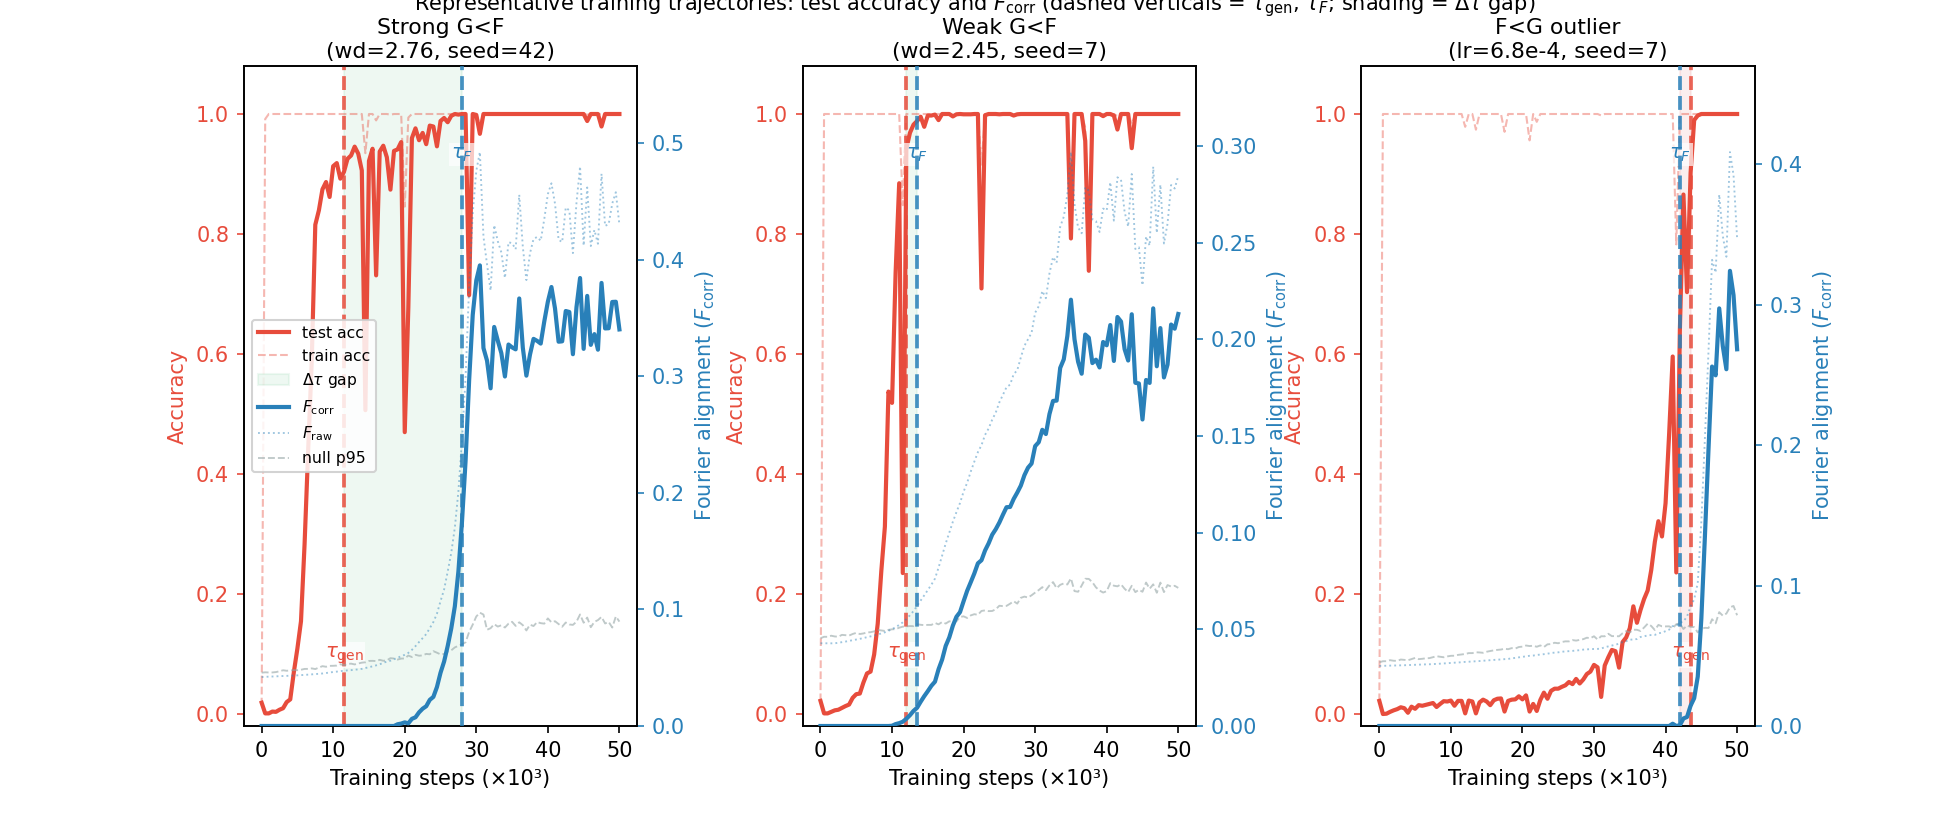
\includegraphics[width=\linewidth]{timeline_example.png}
  \caption{%
    \textbf{Example training trajectories for three representative runs.}
    Red curves: test accuracy (left axis).
    Blue curves: null-corrected Fourier alignment $\fcorr$ (right axis,
    dotted = raw $F_{\mathrm{raw}}$, grey dashed = null p95 baseline).
    Dashed verticals mark $\taug$ (red) and $\tauf$ (blue).
    \emph{Left and centre}: G$<$F runs where generalization fires first
    and the green-shaded $\Dtau$ gap follows;
    $\fcorr$ rises only after test accuracy has already reached~1.
    \emph{Right}: the original Stage~3 F$<$G outlier
    (lr$=6.8\!\times\!10^{-4}$, seed~7), stable under detector
    hyperparameters but not reproduced in the targeted
    cross-hardware re-run of Section~\ref{sec:speed}, where
    $\fcorr$ barely exceeds the null baseline ($0.015$) one
    log-interval before an unusually late $\taug=43{,}500$.
  }
  \label{fig:timeline}
\end{figure}

\subsection{Stage~2: \texorpdfstring{G$<$F}{G<F} Across Weight Decay}
\label{sec:results_wd}

All 30 Stage~2 runs land in the Grokking phase
($\mathrm{train\_acc}=1.0$, $\mathrm{test\_acc}\geq 0.99$).
\textbf{29/30 runs (96.7\%, 95\% CI 83.3\%--99.4\%) show G$<$F
ordering}; the sole exception (wd$=3.11$, seed~2025) has $\Dtau=0$
and is labeled coincident (treated as a tie throughout this paper,
not counted as F$<$G).
\textbf{No Stage~2 run exhibits F$<$G ordering}, so the headline
finding is most precisely stated as ``no F$<$G within the Grokking
phase at the Stage~2 resolution,'' with 29/30 strictly G$<$F and
1/30 tied.
All 95\% confidence intervals reported in Results are Wilson
intervals for a binomial proportion.
Table~\ref{tab:stage2} and Figure~\ref{fig:stage2} summarize the results.
P(G$<$F) remains near~1.0 across the full wd range tested; the median
$\Dtau$ fluctuates between 5{,}500 and 13{,}000 steps with no
monotonic trend, and P(F\_only)$=0$ throughout.

\begin{table}[t]
  \centering
  \caption{Stage~2: wd sweep at $\mathrm{lr}=1.6\times10^{-3}$
    (3~seeds per wd value). All 30~runs are Grokking phase.
    $\Dtau{=}\tauf{-}\taug$ in thousands of steps (positive = G$<$F).
    Medians computed across seeds.}
  \label{tab:stage2}
  \small
  \begin{tabular}{rcccc}
    \toprule
    wd & P(G$<$F) & med.\ $\taug$ (k) & med.\ $\tauf$ (k) & med.\ $\Dtau$ (k) \\
    \midrule
    1.20 & 3/3 & 26.0 & 34.0 & $+7.0$ \\
    1.35 & 3/3 & 20.5 & 28.5 & $+9.0$ \\
    1.52 & 3/3 & 14.5 & 21.5 & $+5.5$ \\
    1.71 & 3/3 & 14.0 & 26.5 & $+6.5$ \\
    1.93 & 3/3 & 14.0 & 23.5 & $+11.0$ \\
    2.18 & 3/3 & 11.0 & 23.5 & $+8.5$ \\
    2.45 & 3/3 & 11.0 & 16.0 & $+5.5$ \\
    2.76 & 3/3 & 10.5 & 18.5 & $+8.5$ \\
    3.11 & 2/3 & 11.0 & 16.5 & $+6.5$ \\
    3.50 & 3/3 & 12.0 & 21.5 & $+9.0$ \\
    \midrule
    \textbf{All} & \textbf{29/30} & --- & --- & $+7.8$ \\
    \bottomrule
  \end{tabular}
\end{table}

\begin{figure}[t]
  \centering
  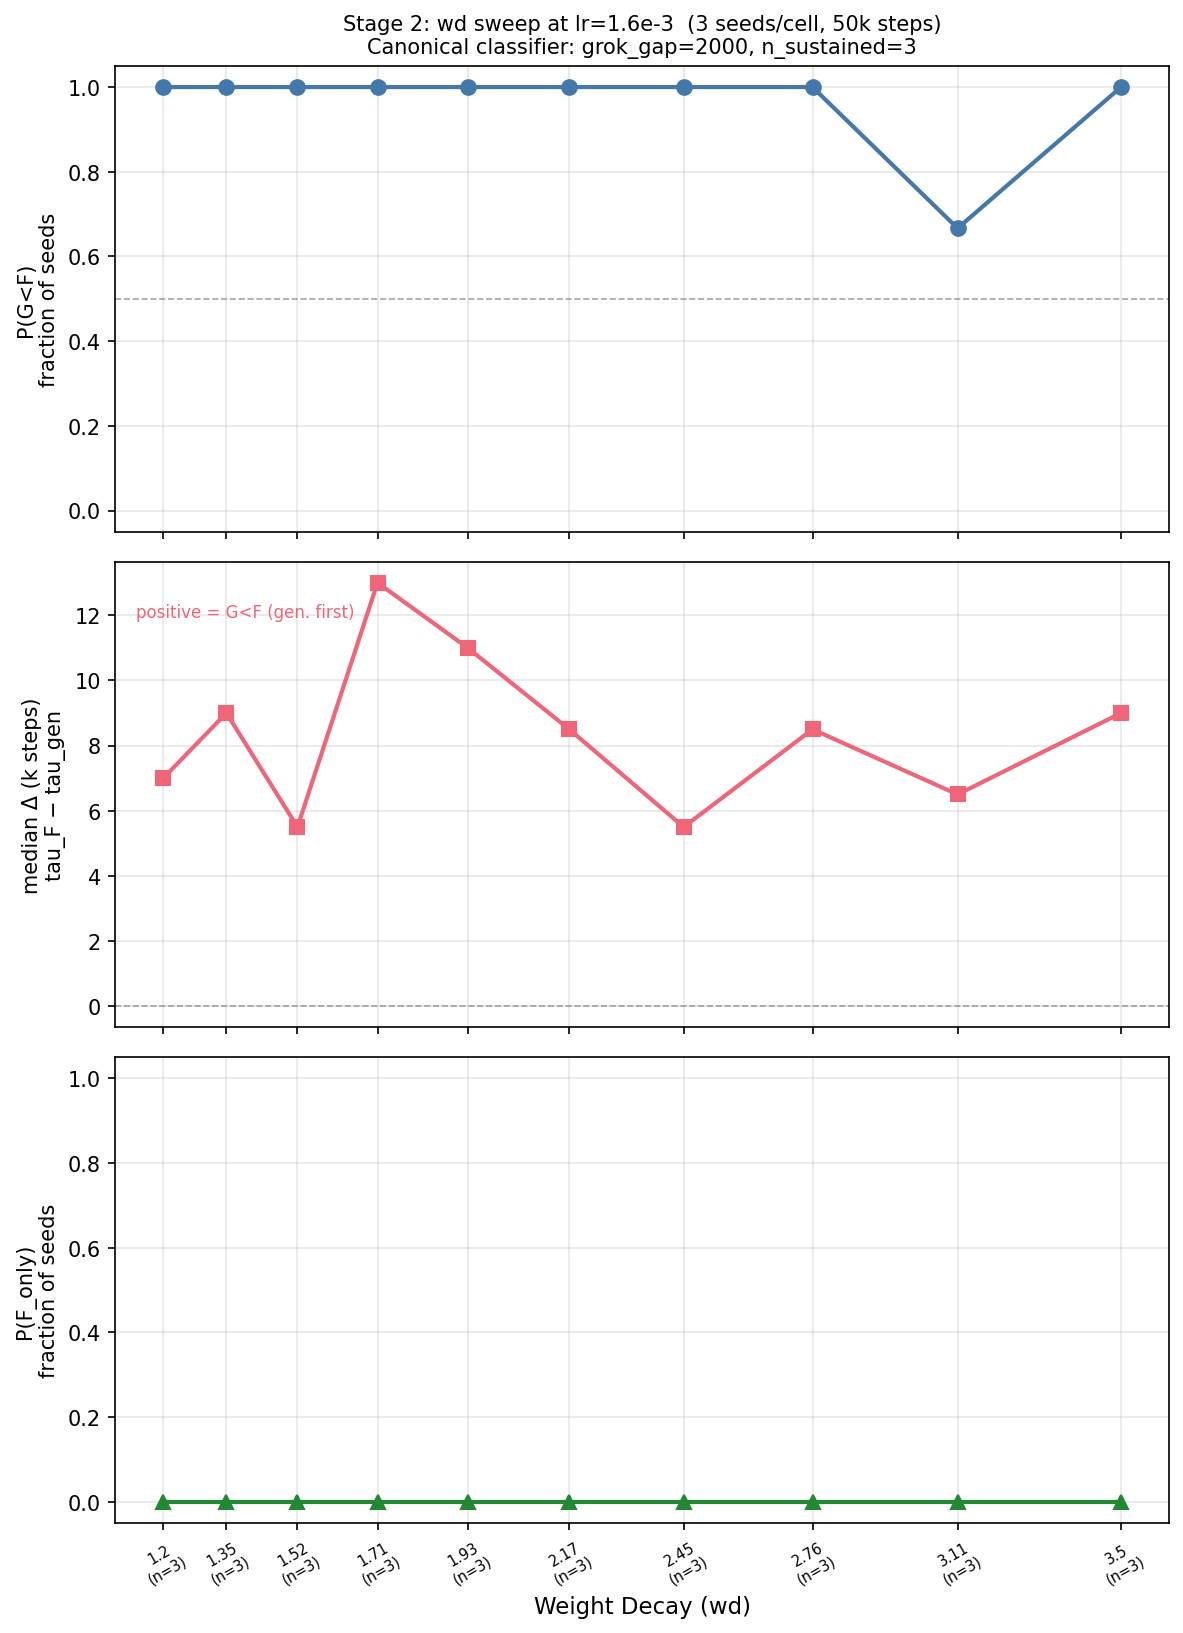
\includegraphics[width=0.82\linewidth]{wd_sweep_curves.png}
  \caption{Stage~2: embedding Fourier consolidation vs.\ generalization
    across weight decay. \textbf{Top}: P(G$<$F) per wd value.
    \textbf{Middle}: median $\Dtau{=}\tauf{-}\taug$ (k~steps).
    \textbf{Bottom}: P(F\_only) (Fourier detected, no generalization).
    The G$<$F plateau is wide: it holds throughout wd $\in[1.2,3.5]$.}
  \label{fig:stage2}
\end{figure}

\subsection{Stage~3: \texorpdfstring{G$<$F}{G<F} Across Learning Rate}
\label{sec:results_lr}

Of the 30 Stage~3 runs, \textbf{25 land in the Grokking phase}
for lr$\in[5\times10^{-4},\,4.3\times10^{-3}]$; the remaining
5~runs (lr$\geq5.9\times10^{-3}$) are Memorization.
Among the 25~Grokking runs, \textbf{23/25 (92.0\%, CI 75.0\%--97.8\%)
show G$<$F ordering}.
Results appear in Table~\ref{tab:stage3} and Figure~\ref{fig:stage3}.

\begin{table}[t]
  \centering
  \caption{Stage~3: lr sweep at $\mathrm{wd}=2.5$
    (3~seeds per lr). ``Phase'' = majority phase across seeds.
    ``---'' = Memorization (no $\taug$ detected).}
  \label{tab:stage3}
  \small
  \begin{tabular}{lcccc}
    \toprule
    lr & Phase & P(G$<$F) & med.\ $\Dtau$ (k) & P(F\_only) \\
    \midrule
    $5.0\times10^{-4}$ & Grokking      & 3/3 & $+2.5$ & 0/3 \\
    $6.8\times10^{-4}$ & Grokking      & 2/3 & $+4.0$ & 0/3 \\
    $9.3\times10^{-4}$ & Grokking      & 3/3 & $+7.5$ & 0/3 \\
    $1.26\times10^{-3}$ & Grokking     & 3/3 & $+9.5$ & 0/3 \\
    $1.71\times10^{-3}$ & Grokking     & 3/3 & $+6.0$ & 0/3 \\
    $2.33\times10^{-3}$ & Grokking     & 3/3 & $+4.0$ & 0/3 \\
    $3.17\times10^{-3}$ & Grokking     & 3/3 & $+6.0$ & 0/3 \\
    $4.32\times10^{-3}$ & Grokking     & 2/3 & $+7.5$ & 0/3 \\
    $5.88\times10^{-3}$ & Mixed        & 1/1 & $+2.5$ & 2/3 \\
    $8.00\times10^{-3}$ & Memorization & ---   & ---      & 3/3 \\
    \midrule
    \textbf{Grokking} & --- & \textbf{23/25} & $+4.0$ & 0/25 \\
    \bottomrule
  \end{tabular}
\end{table}

\begin{figure}[!t]
  \centering
  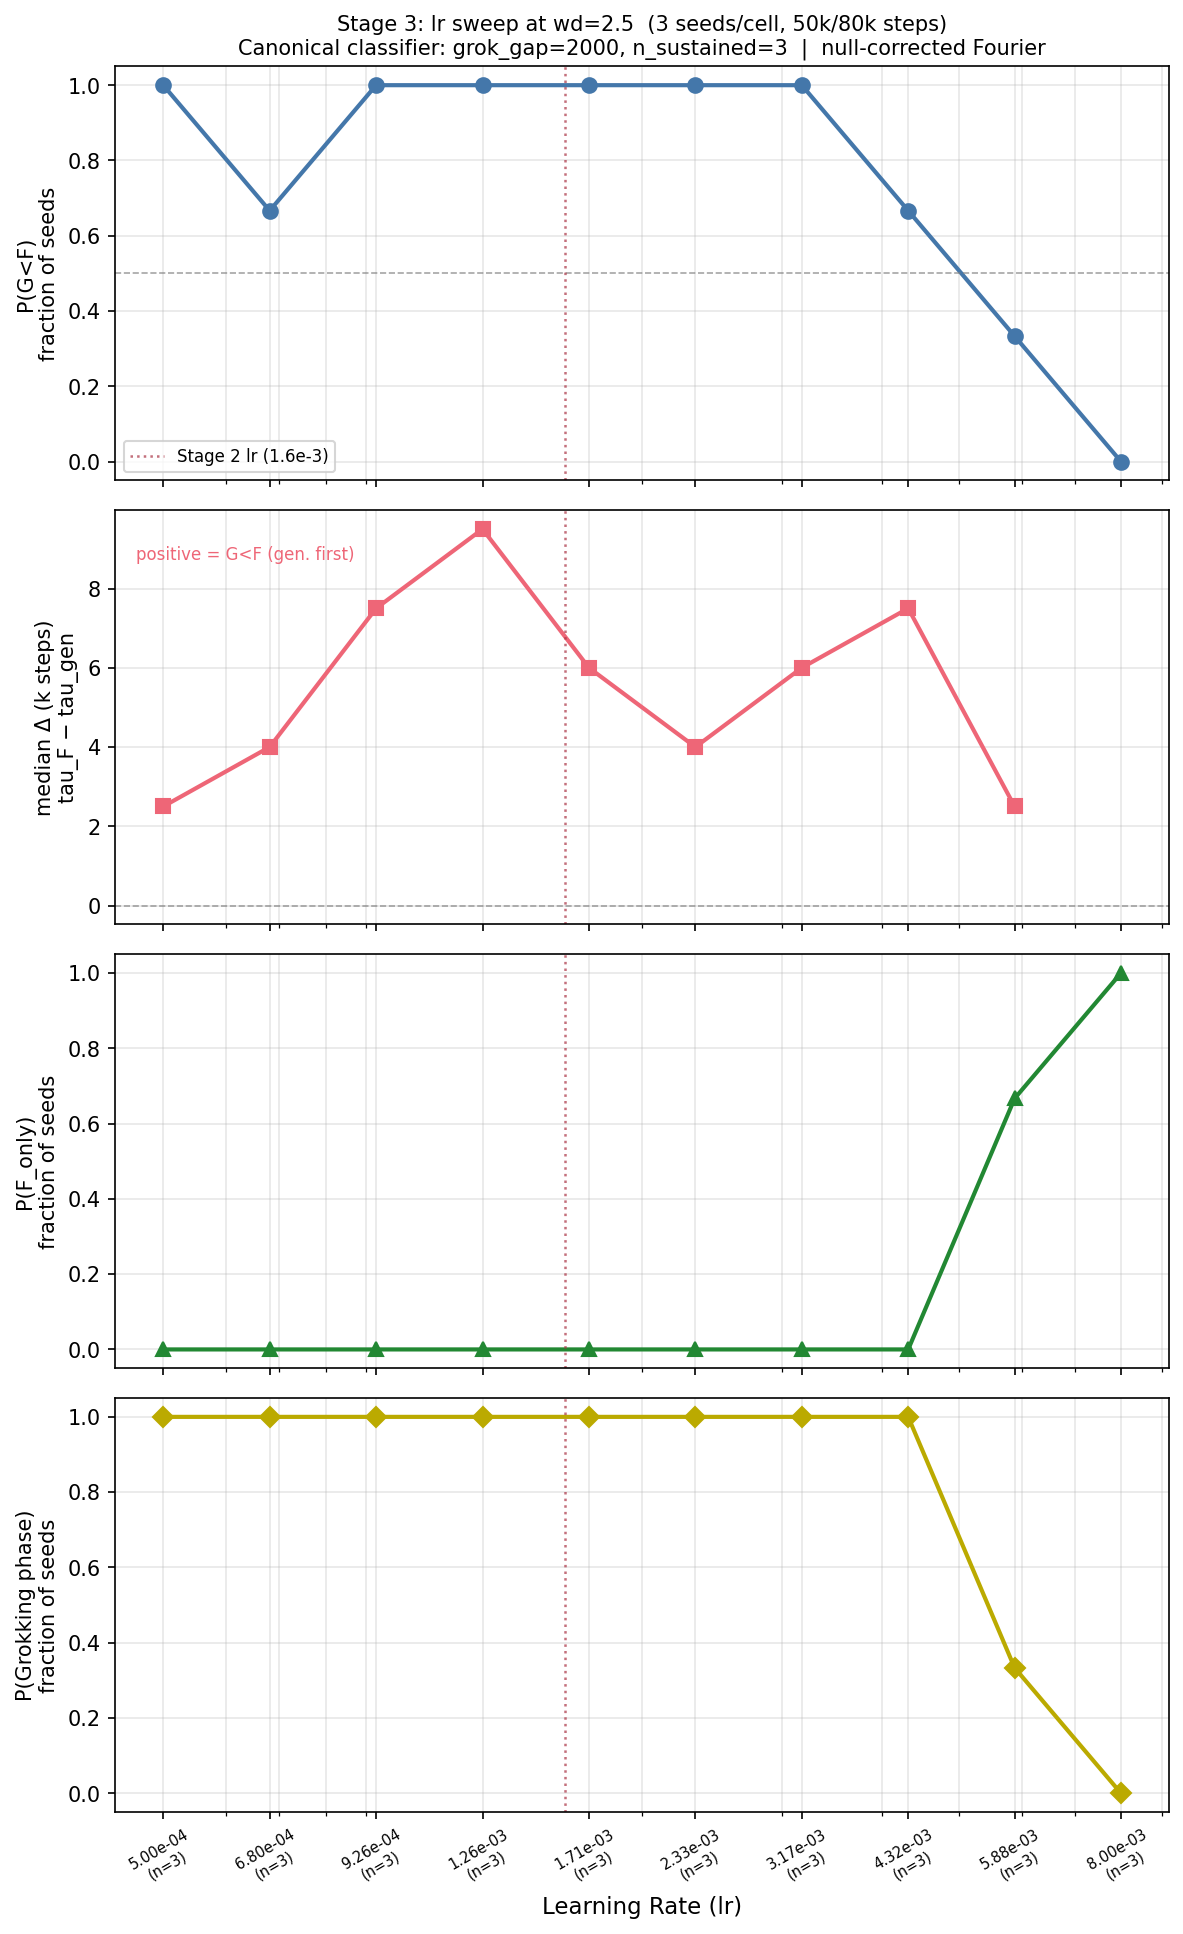
\includegraphics[width=0.72\linewidth]{lr_sweep_curves.png}
  \caption{Stage~3: embedding Fourier consolidation vs.\ generalization
    across learning rate ($\mathrm{wd}=2.5$). Layout mirrors
    Figure~\ref{fig:stage2}; x-axis is log-scaled.
    The bottom panel shows P(Grokking) per lr: cells at
    lr$\geq5.9\times10^{-3}$ enter Memorization.
    The vertical dotted line marks the Stage~2 fixed lr
    ($1.6\times10^{-3}$), which lies firmly in the G$<$F plateau.}
  \label{fig:stage3}
\end{figure}

The two exceptions to G$<$F deserve comment.
\textbf{(i)}~lr$=6.8\times10^{-4}$, seed~7: $\Dtau=-1{,}500$~steps,
above the 500-step resolution floor but spanning only 3 checkpoints;
the sensitivity analysis confirms F$<$G is stable across all 36 detector
configurations (see Section~\ref{sec:robustness}).
\textbf{(ii)}~lr$=4.32\times10^{-3}$, seed~42: $\Dtau=-54{,}500$~steps
and max test accuracy only 0.965 (required 80k-step extension).
This seed sits at the edge of the Grokking phase and had an atypical
training trajectory.

\subsection{Combined: \texorpdfstring{$\Dtau$}{Delta tau} Distribution}
\label{sec:combined}

Combining both sweeps, 55 of 60 runs land in the Grokking phase.
Of these, \textbf{52/55 (94.5\%, CI 85.1\%--98.1\%) show G$<$F
ordering}, 2/55 show F$<$G, and 1/55 is coincident ($\Dtau=0$).
Figure~\ref{fig:delta_hist} shows the full $\Dtau$ distribution.
Positive values (G$<$F) span 1{,}000--25{,}500 steps;
the two negative values are the outliers noted above.
Median $\Dtau\approx7{,}000$~steps (IQR $\approx4{,}000$~steps).

\begin{figure}[t]
  \centering
  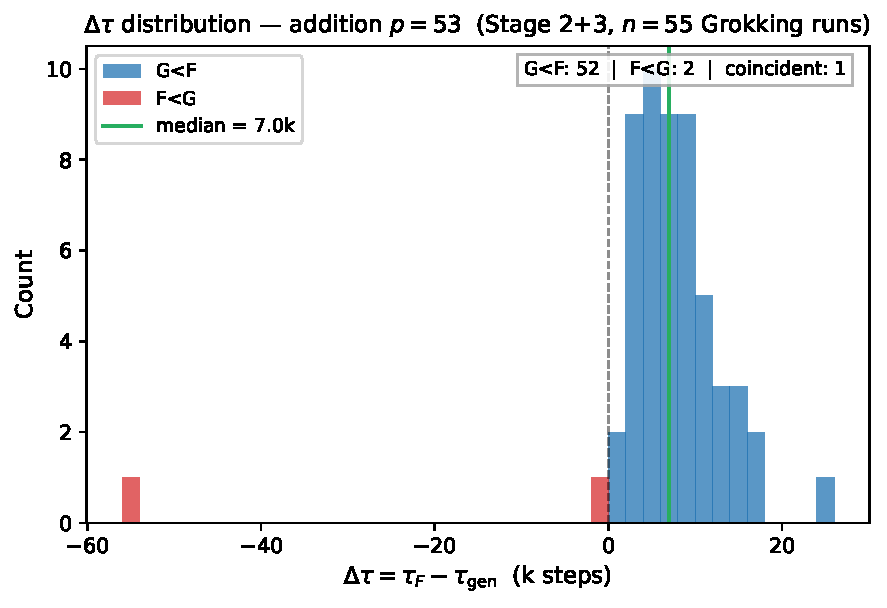
\includegraphics[width=0.80\linewidth]{delta_histogram.pdf}
  \caption{Distribution of $\Dtau{=}\tauf{-}\taug$ across all
    55~Grokking runs (Stage~2 blue, Stage~3 red).
    Positive values indicate G$<$F (generalization first).
    Median $\Dtau\approx7{,}000$~steps; 52/55 runs (94.5\%) are
    positive. The two negative values are discussed in
    Section~\ref{sec:results_lr}.}
  \label{fig:delta_hist}
\end{figure}

\subsection{Stage~4: Circuit Onset \texorpdfstring{$\taucirc$}{tau\_circuit} and Three-Stage Ordering}
\label{sec:results_circuit}

We retrained all Stage~2+3 cells with the additional $\flogit$ metric,
yielding $\taucirc$ for each run.
$\taucirc$ was detected in all 54~Grokking runs (100\%).

\paragraph{C$\leq$G (circuit at or before generalization).}
In 49/54 Grokking runs (90.7\%), $\taucirc < \taug$ strictly;
in one additional run $\taucirc = \taug$ (both detected at the
same 500-step checkpoint), giving 50/54 (92.6\%, CI
82.4\%--97.1\%) under the C$\leq$G convention used throughout
this section.
The median gap $\taug - \taucirc \approx 6{,}250$~steps
(range $-3{,}000$ to $35{,}000$~steps).
The 4~exceptions with $\taucirc > \taug$ (i.e.\ G$<$C$<$F) occur
at the highest learning rates (lr$\geq2.3\times10^{-3}$, wd$=2.5$),
where generalization is very fast ($\taug \leq 6{,}500$~steps) and
the logit Fourier signal rises too gradually for BIC to detect a
changepoint before $\taug$.

\paragraph{Proxy-level three-stage ordering C$<$G$<$F.}
The dominant pattern is \textbf{C$<$G$<$F} in 48/54 runs
(88.9\%, CI 77.8\%--94.8\%).
The remaining runs split into C$<$F$<$G (2 runs, low-lr boundary)
and G$<$C$<$F (4 runs, high-lr boundary).
The three intervals are nearly equal in magnitude:
median $\taug - \taucirc \approx 6{,}250$~steps,
median $\tauf - \taug \approx 6{,}000$~steps,
median $\tauf - \taucirc \approx 13{,}000$~steps.

\begin{figure}[t]
  \centering
  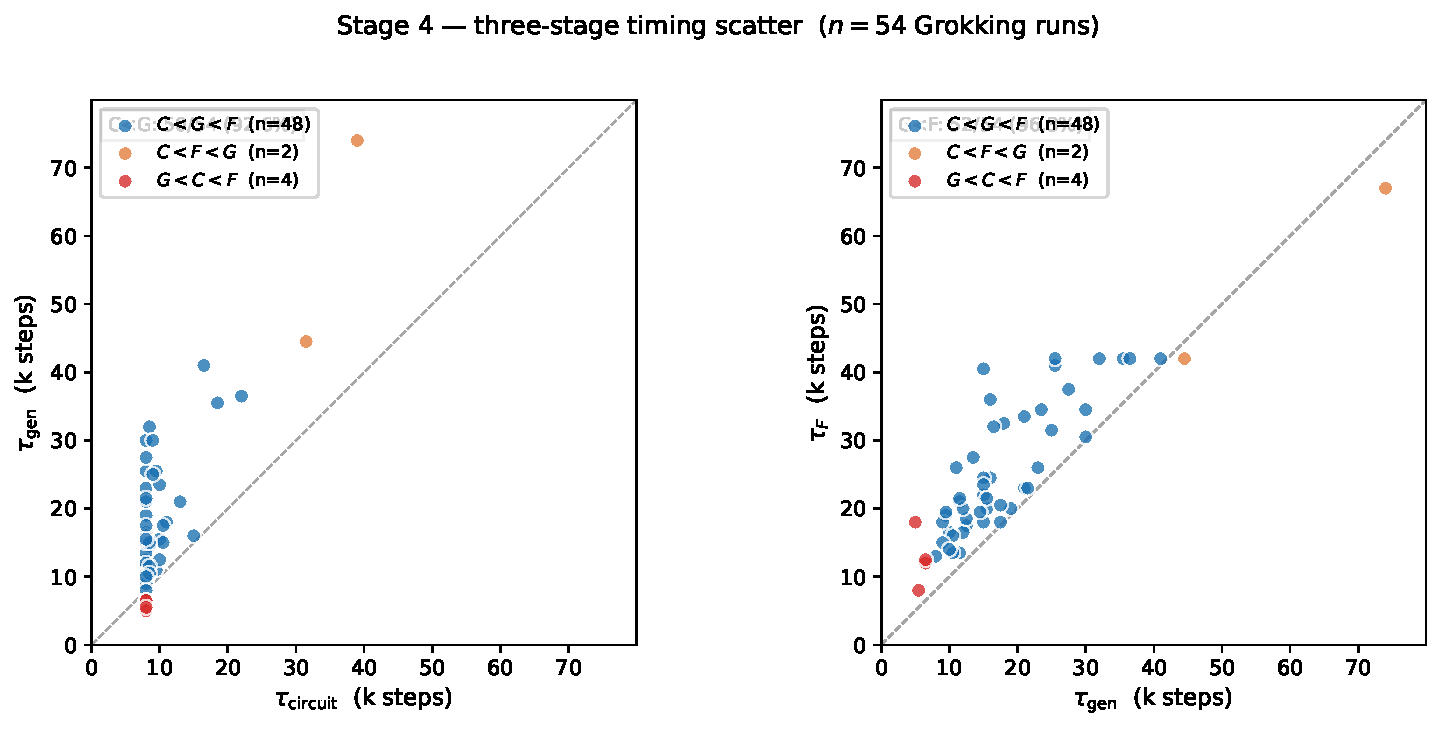
\includegraphics[width=\linewidth]{step2_three_stage_scatter.pdf}
  \caption{%
    \textbf{Three-stage timing scatter (Stage~4).}
    \emph{Left}: $\taucirc$ (circuit) vs $\taug$ (generalization).
    Points above the diagonal ($y>x$) confirm C$<$G ordering.
    Blue: C$<$G$<$F (dominant); orange: C$<$F$<$G; pink: G$<$C$<$F.
    \emph{Right}: $\taug$ vs $\tauf$ (embedding geometry).
    Points above diagonal confirm G$<$F.
    C$<$G holds marginally in 50/54 runs (92.6\%); the stricter
    joint C$<$G$<$F pattern in Table~\ref{tab:step2} requires
    both C$<$G and G$<$F in the same run.
  }
  \label{fig:step2_scatter}
\end{figure}

\begin{figure}[t]
  \centering
  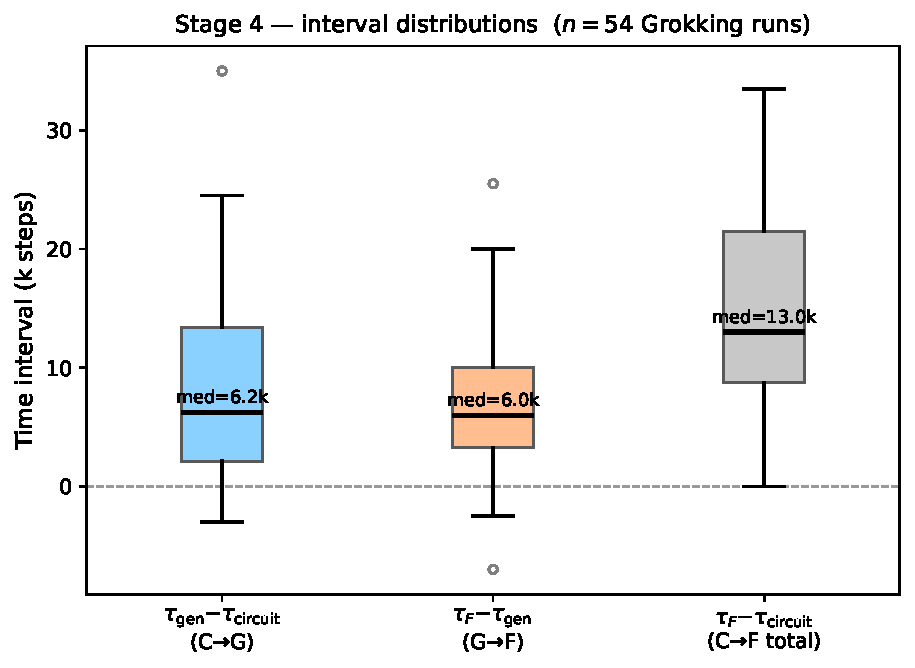
\includegraphics[width=0.65\linewidth]{step2_interval_boxplot.pdf}
  \caption{%
    \textbf{Three-stage interval distributions (Stage~4, $n{=}54$ Grokking runs).}
    All three intervals are positive on the median, with the total span
    $\tauf-\taucirc\approx13{,}000$ steps split nearly equally between
    circuit$\to$generalization and generalization$\to$embedding-geometry.
  }
  \label{fig:step2_boxplot}
\end{figure}

\begin{table}[t]
  \centering
  \caption{Stage~4: three-stage timing across Stage~2 (lr$=1.6\times10^{-3}$)
    and Stage~3 (wd$=2.5$) Grokking runs.
    Medians in thousands of steps.}
  \label{tab:step2}
  \small
  \begin{tabular}{lcccc}
    \toprule
    Subset & C$<$G$<$F & C$<$G$<$F rate & med.\ $\taug{-}\taucirc$ (k) & med.\ $\tauf{-}\taug$ (k) \\
    \midrule
    Stage~2 (lr fixed) & 30/30 & 100\% & $6.3$ & $6.0$ \\
    Stage~3 (wd fixed) & 18/24 & 75.0\%  & $6.3$ & $6.0$ \\
    \midrule
    \textbf{All} & \textbf{48/54} & \textbf{88.9\%} & $\mathbf{6.3}$ & $\mathbf{6.0}$ \\
    \bottomrule
  \end{tabular}
\end{table}

\subsection{Stage~5A: Modular Multiplication}
\label{sec:results_mul}

All 30~runs with $(a\cdot b)\bmod 53$ land in the Grokking phase.
\textbf{30/30 (100\%, CI 88.6\%--100\%) show G$<$F ordering} after
discrete-log reindexing of token embeddings.
Median $\Dtau = 8{,}750$~steps (range 3{,}500--24{,}000), comparable
to the addition results.
The perfect G$<$F rate extends the finding beyond the addition task,
suggesting the ordering is not specific to the $(a+b)\bmod p$ circuit
structure.

\paragraph{Evaluation-domain check.}
$\taug$ in the Stage~5A headline is computed from the standard
$70/30$ random split over the full $p^{2}$ input pairs (including
pairs with a zero operand), whereas $\fcorr$ and $\flogit$ (and
hence $\tauf$ and $\taucirc$) are restricted to the
$\mathbb{F}_p^*$ subgrid
(Section~\ref{sec:methods}, ``Stage~5A --- modular multiplication'').
To verify that this evaluation-domain mismatch does not inflate
the reported G$<$F rate, we re-ran the full $30$-cell Stage~5A
sweep with identical seeds and additionally tracked test accuracy
on the $\mathbb{F}_p^*$-only test subset
($a, b \in \{1, \dots, p-1\}$) at every $500$-step checkpoint
(\texttt{src/sweeps/stage5a\_fpstar\_recompute.py};
results in \texttt{results/stage5a\_fpstar/results.csv}).
The recompute confirms that the matched-domain $\taug$ is almost
identical to the full-split $\taug$:
$\tau_{\mathrm{gen}}^{\mathbb{F}_p^*}-\tau_{\mathrm{gen}}^{\mathrm{full}}
\in\{0, 500\}$ steps for all $30$ cells (median $0$, max $500$,
i.e.\ at most one $500$-step measurement bin), the median
$\Dtau$ is unchanged at $8{,}750$ steps, the minimum
$|\Dtau^{\mathbb{F}_p^*}|$ is $3{,}500$ steps, and the
$30/30$ G$<$F rate is preserved (no cell flips to coincident or
F$<$G).
The Stage~5A G$<$F claim is therefore not an artefact of the
evaluation-domain mismatch; the same caveat does not apply to
Stage~5B, Stage~2, Stage~3, Stage~4, or Stage~6, all of which use
the full-vocabulary additive group $\mathbb{Z}/p$ and have no
analogous trivial subgrid.

\subsection{Stage~5B: Different Prime (\texorpdfstring{$p{=}97$}{p=97})}
\label{sec:results_p97}

Of the 30 runs with $(a+b)\bmod 97$, 21 land in the Grokking phase
(9 in Comprehension, concentrated at high wd where fast generalization
prevents a Grokking-phase classification).
\textbf{21/21 Grokking runs (100\%, CI 84.5\%--100\%) show G$<$F
ordering.}
The median lag $\Dtau = 28{,}000$~steps is markedly larger than for
$p{=}53$ ($\approx7{,}000$~steps), consistent with the larger prime
requiring more training steps and a correspondingly longer
consolidation period.
The G$<$F rate and direction are unchanged.

\begin{table}[t]
  \centering
  \caption{G$<$F rates across all experimental stages.
    $n_G$: Grokking runs; G$<$F: ordering rate and median lag.
    95\% CIs are Wilson intervals for a binomial proportion.
    The ``All (main stages)'' row excludes the targeted
    slow-grokking sweep of Section~\ref{sec:speed} (which adds
    24/24 G$<$F cells and brings the aggregate to
    $236/260{=}90.8\%$).
    A cell-level cluster bootstrap
    (Table~\ref{tab:cluster_bootstrap}) yields 33--40\% wider CIs
    on sources with non-degenerate seed clustering; point estimates
    shift by $<$1\%.}
  \label{tab:summary_all}
  \small
  \begin{tabular}{llcccc}
    \toprule
    Stage & Setting & $n_G$ & G$<$F rate & 95\% CI & med.\ $\Dtau$ (k) \\
    \midrule
    2+3  & add mod 53, 1D sweeps & 55  & 94.5\%  & 85.1--98.1\% & $7.0$ \\
    5A   & mul mod 53            & 30  & \textbf{100\%}   & 88.6--100\% & $8.8$ \\
    5B   & add mod 97            & 21  & \textbf{100\%}   & 84.5--100\% & $28.0$ \\
    6    & add mod 53, 2D grid   & 130 & 83.8\%  & 76.6--89.2\% & $6.0$ \\
    \midrule
    \textbf{All (main stages)} & & \textbf{236} & \textbf{89.8\%} & \textbf{85.3--93.1\%} & --- \\
    \midrule
    \S\ref{sec:speed} & slow-grokking sweep (post-hoc) & 24  & \textbf{100\%}   & 86.2--100\% & $11.75$ \\
    \midrule
    \textbf{All (incl.\ slow-grokking sweep)} & & \textbf{260} & \textbf{90.8\%} & \textbf{86.6--93.7\%} & --- \\
    \bottomrule
  \end{tabular}
\end{table}

\begin{figure}[t]
  \centering
  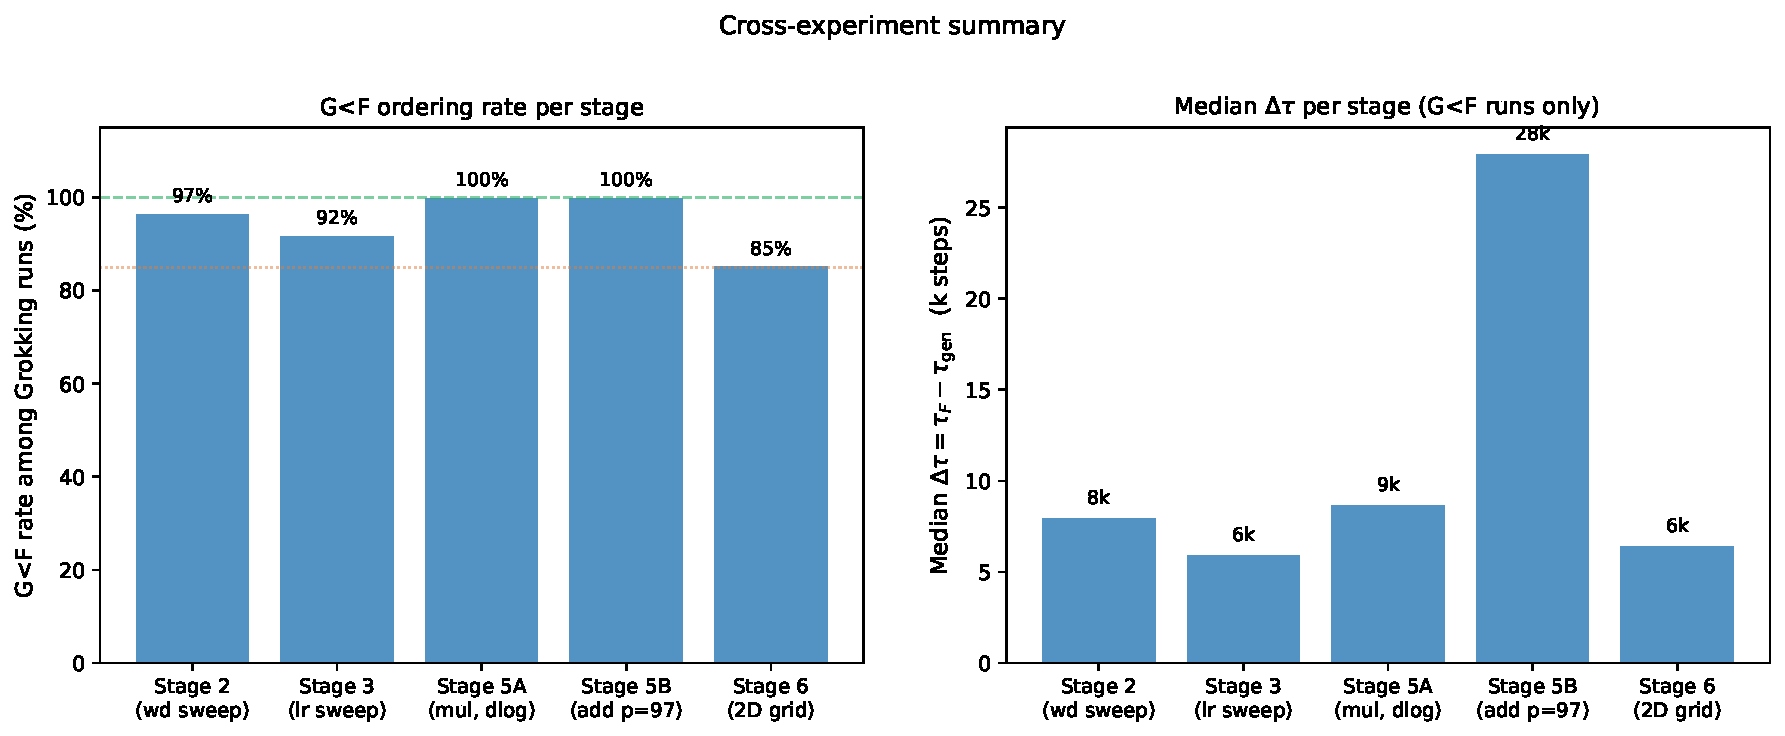
\includegraphics[width=\linewidth]{cross_experiment_summary.pdf}
  \caption{%
    \textbf{G$<$F rate and median lag across all experimental stages.}
    \emph{Left}: G$<$F ordering rate; all stages exceed 85\%.
    \emph{Right}: median $\Dtau{=}\tauf{-}\taug$; the larger prime $p{=}97$
    (Stage~5B) shows a markedly larger lag, consistent with slower grokking
    requiring a longer consolidation period.
  }
  \label{fig:cross_summary}
\end{figure}

\subsection{Stage~6: \texorpdfstring{G$<$F}{G<F} Across the Full 2D Phase Diagram}
\label{sec:results_2d}

The 7$\times$7 grid yields 130~Grokking runs (88.4\% of 147 total;
16 Memorization, 1 Comprehension).
\textbf{109/130 Grokking runs (83.8\%, CI 76.6\%--89.2\%) show G$<$F
ordering} under the canonical $|\Dtau|\leq 500$ coincident
threshold; 13/130 show F$<$G, 3/130 are coincident, and
5/130 have G\_only ($\tauf$ not
detected).
Median $\Dtau \approx 6{,}000$~steps.

The G$<$F rate is not uniform across the grid.
By learning rate, G$<$F peaks at intermediate lr ($\approx$95\% for
lr$\in[10^{-3},\,2\times10^{-3}]$) and decreases toward both
boundaries (58\% at lr$=5\times10^{-4}$, 78\% at lr$=4.3\times10^{-3}$).
By weight decay, G$<$F increases monotonically from 72\% at wd$=1.43$
to 95\% at wd$\geq2.93$.
F$<$G cases concentrate at the low-lr and high-lr boundaries (12
of 14 cases under the original detector-only ordering label, 11
of 13 under the canonical $|\Dtau|\leq500$ coincident threshold).
This boundary clustering initially motivated the speed-dependent
ordering hypothesis tested in Section~\ref{sec:speed}; the
targeted slow-grokking sweep there falsifies its strong form.
We therefore treat these Stage~6 boundary cases as phase-margin
irregularities (likely seed/hardware-level fluctuations and
detector-resolution artefacts) rather than evidence for a
systematic F$<$G regime.
The interior of the Grokking phase is robustly G$<$F.
Figure~\ref{fig:stage6_heatmap} shows the full spatial structure.

\begin{figure}[t]
  \centering
  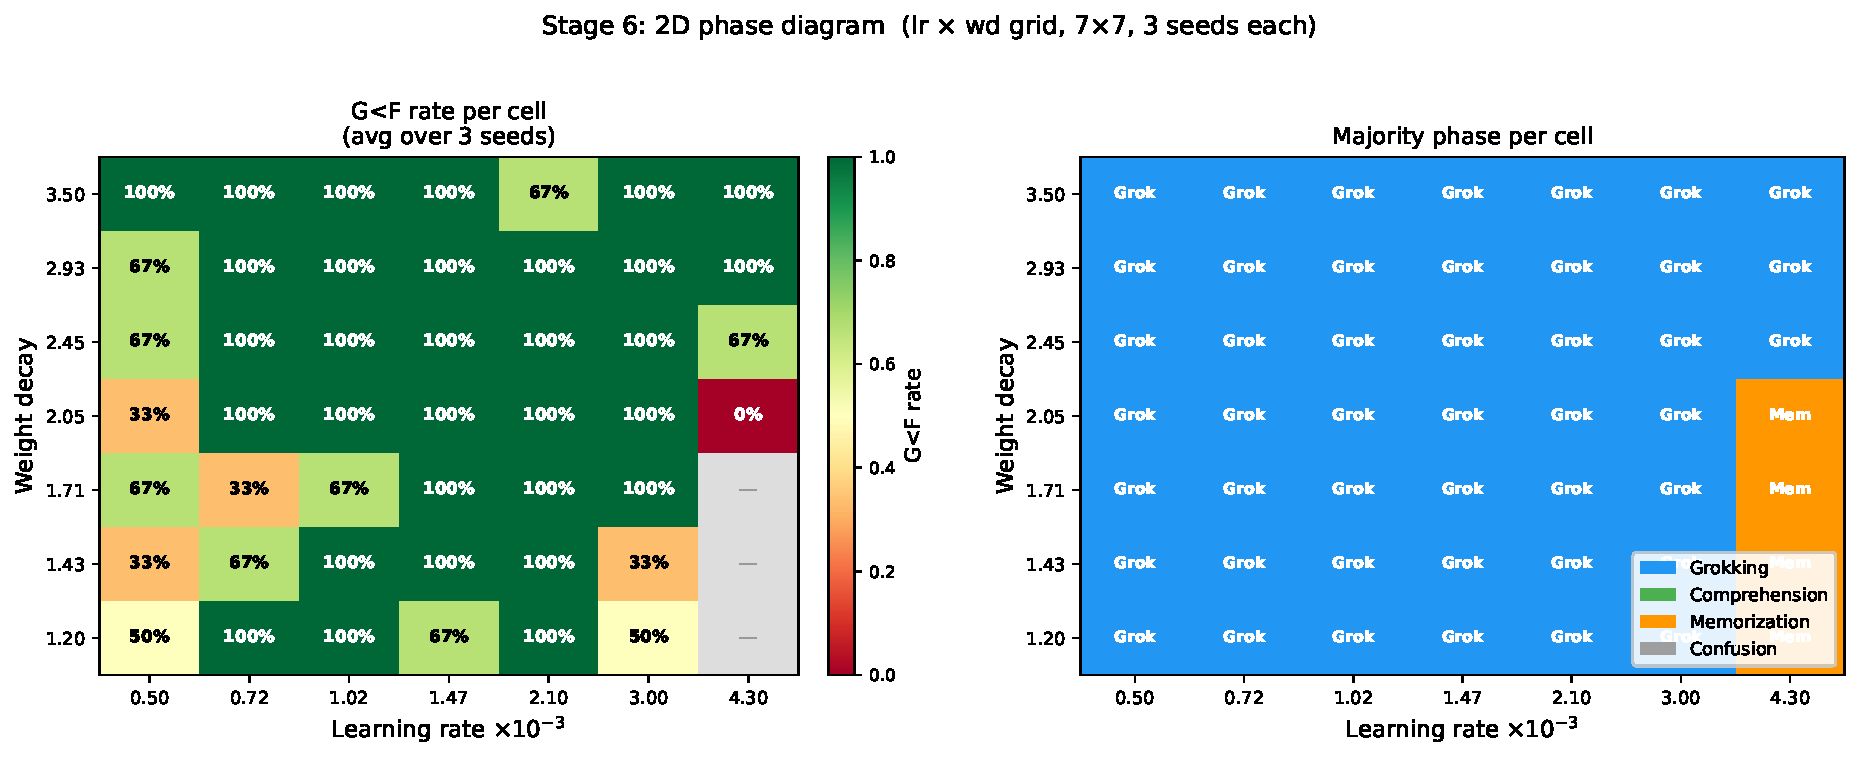
\includegraphics[width=\linewidth]{stage6_2d_heatmap.pdf}
  \caption{%
    \textbf{Stage~6: 2D phase diagram and G$<$F rate.}
    \emph{Left}: G$<$F rate per (lr, wd) cell, averaged over 3~seeds.
    G$<$F is strongest in the interior (lr$\in[10^{-3},\,2\times10^{-3}]$,
    wd$\geq2.5$) and weakens toward phase boundaries.
    \emph{Right}: majority phase per cell.
    Memorization occupies the high-lr, low-wd corner.
  }
  \label{fig:stage6_heatmap}
\end{figure}

\subsection{Decoupled Weight-Decay Ablation}
\label{sec:e4_ablation}

\emph{The two ablations in this section identify the conditions
that produce the timing dissociation: E4 isolates the
optimizer-side pathway that generates the lag and locates the
regime boundary, and E5 varies generalization speed through the
data path while holding that pathway fixed.}

The canonical sweep applies weight decay only to the decoder
parameter group; embedding parameters are by default excluded.
To distinguish whether the G$<$F ordering is driven by decoder
weight decay, by embedding weight decay, or by their interaction,
and to localise \emph{when} the decay pressure matters, we run two
coupled ablations at the canonical operating point
$(\mathrm{lr},\mathrm{wd}^{\star}){=}(1.6{\times}10^{-3},\,2.5)$
with $\taug^{\mathrm{ref}}{=}17{,}000$
(source: \texttt{src/sweeps/e4\_decoupled\_wd.py},
results in \texttt{results/e4/results.csv}).

\paragraph{$2\times 2$ ablation ---
$(\mathrm{wd}_{\mathrm{dec}},\mathrm{wd}_{\mathrm{emb}})\in\{0,\mathrm{wd}^{\star}\}^{2}$.}
Three seeds per cell, 12~runs total.
Table~\ref{tab:e4_2x2} reports the per-cell phase distribution
and ordering.
Three observations follow, each conditional on the canonical
$(\mathrm{lr},\mathrm{wd}^{\star})$ operating point and 3 seeds
per cell.
\textbf{(i)~$\mathrm{wd}_{\mathrm{dec}}{=}0$ abolishes grokking
under this canonical setting}: both cells with zero decoder decay
memorise in all 3 seeds (max test accuracy $\leq 0.10$).
Decoder weight decay therefore appears \emph{necessary} for
grokking under this canonical operating point; we read this as a
local causal statement, not a universal one.
The $(0, \mathrm{wd}^{\star})$ cell is informative for a separate
reason: despite direct weight decay on the embedding parameters,
it produces $\tauf$ but no $\taug$ (F\_only phase).
This provides direct evidence that embedding Fourier alignment is
\emph{not sufficient} for generalisation, and the headline G$<$F
result rules out the converse reading as well: with $\tauf$
falling \emph{after} $\taug$ in $212/236$ Grokking runs, ring
consolidation cannot be a temporal prerequisite for
generalisation either.
\textbf{(ii)~$\mathrm{wd}_{\mathrm{dec}}{=}\mathrm{wd}^{\star}$
alone reproduces canonical G$<$F}: the
$(\mathrm{wd}^{\star},0)$ cell groks in all 3 seeds with mean
$\Dtau{=}6{,}500$ steps, matching the Stage~2 G$<$F plateau.
\textbf{(iii)~Adding $\mathrm{wd}_{\mathrm{emb}}{=}\mathrm{wd}^{\star}$
on top of $\mathrm{wd}_{\mathrm{dec}}{=}\mathrm{wd}^{\star}$
destabilises the canonical dynamics}: 1/3 seeds memorises, and
the 2/3 that grok do so with $\tauf\in\{8{,}000,10{,}000\}$,
arriving \emph{before} $\taug\in\{19{,}500,16{,}000\}$ --- an
F$<$G ordering, reproducibly.
Direct embedding decay therefore accelerates Fourier consolidation
enough to precede generalisation, giving a second reproducible
recipe for F$<$G beyond the low-lr regime
observed in Stage~3.
Taken together, the $2\times 2$ results reframe our central claim:
\emph{decoder-only weight decay} is the operating point under
which G$<$F is observed; ``weight decay drives grokking'' is
more accurately stated as ``\emph{decoder} weight decay drives
grokking, and combining it with embedding decay flips the
ordering''.

\begin{table}[tbp]
  \centering
  \caption{E4a --- $2{\times}2$ weight-decay ablation (3 seeds per
    cell).
    Phase counts are over the 3 seeds.
    For Grokking seeds the range of
    $(\taug,\,\tauf,\,\Dtau)$ is reported.
    Source: \texttt{results/e4/results.csv}.}
  \label{tab:e4_2x2}
  \small
  \begin{tabular}{cccccc}
    \toprule
    $\mathrm{wd}_{\mathrm{dec}}$ & $\mathrm{wd}_{\mathrm{emb}}$ &
    phase (3 seeds) & $\taug$ & $\tauf$ & ordering \\
    \midrule
    $0$              & $0$              & Mem $\times 3$              & --                & --                  & none \\
    $0$              & $\mathrm{wd}^{\star}$ & Mem $\times 3$         & --                & $[8{,}000,\,28{,}500]$ & F\_only \\
    $\mathrm{wd}^{\star}$ & $0$         & Grok $\times 3$             & $[10{,}000,\,13{,}500]$ & $[15{,}000,\,23{,}500]$ & G$<$F \\
    $\mathrm{wd}^{\star}$ & $\mathrm{wd}^{\star}$ & Mem+Grok$\times 2$ & $[16{,}000,\,19{,}500]$ & $[8{,}000,\,10{,}000]$ & F$<$G \\
    \bottomrule
  \end{tabular}
\end{table}

\paragraph{Decoder-WD shutoff schedule.}
Starting from the canonical
$(\mathrm{wd}_{\mathrm{dec}},\mathrm{wd}_{\mathrm{emb}})
{=}(\mathrm{wd}^{\star},0)$ configuration, we set
$\mathrm{wd}_{\mathrm{dec}}{=}0$ at step
$s^{\star}\in\{0.5,1,2\}\cdot\taug^{\mathrm{ref}}$
(3 seeds each, 9~runs).
Results in Table~\ref{tab:e4_schedule} localise the causal window.
Shutoff at $0.5\taug^{\mathrm{ref}}{=}8{,}500$, \emph{before} the
canonical $\taug$, eliminates grokking in all 3 seeds: max test
accuracy plateaus at $0.47$--$0.73$ (still a partial progress
signal, but never crossing the $0.9$ threshold used for $\taug$).
Shutoff at $\taug^{\mathrm{ref}}$ and at $2\taug^{\mathrm{ref}}$
both preserve canonical grokking, with G$<$F in 3/3 seeds at each
shutoff time.
Decoder weight decay therefore appears to act \emph{locally
causally} during the pre-$\taug$ window: removing it within
$[0,\,\taug)$ abolishes grokking, while shutting it off after
$\taug$ does not rescind generalisation. Prolonged
decay past $\taug$ delays $\tauf$ (median $\tauf$ at shutoff
$2\taug^{\mathrm{ref}}$ is $29{,}000$ vs.\ $17{,}000$ at
$\taug^{\mathrm{ref}}$), consistent with decay continuing to
suppress the magnitude signal that drives the BIC changepoint.

\begin{table}[tbp]
  \centering
  \caption{E4b --- Decoder-WD shutoff schedule (3 seeds each) at
    $\taug^{\mathrm{ref}}{=}17{,}000$.
    Source: \texttt{results/e4/results.csv}.}
  \label{tab:e4_schedule}
  \small
  \begin{tabular}{ccccc}
    \toprule
    shutoff step & phase (3 seeds) & $\taug$ range & $\tauf$ range & max test acc \\
    \midrule
    $8{,}500$ ($0.5\taug^{\mathrm{ref}}$)  & Mem $\times 3$  & --                      & $[21{,}500,\,24{,}000]$ & $0.47$--$0.73$ \\
    $17{,}000$ ($\taug^{\mathrm{ref}}$)    & Grok $\times 3$ & $[10{,}000,\,13{,}500]$ & $[16{,}000,\,17{,}500]$ & $1.00$ \\
    $34{,}000$ ($2\taug^{\mathrm{ref}}$)   & Grok $\times 3$ & $[10{,}000,\,13{,}500]$ & $[16{,}000,\,29{,}500]$ & $1.00$ \\
    \bottomrule
  \end{tabular}
\end{table}

Together these two ablations identify decoder weight decay as the
optimizer-side condition that puts the network into the grokking
regime under the tested conditions: within the canonical
operating point
$(\mathrm{lr},\mathrm{wd}^{\star}){=}(1.6{\times}10^{-3},\,2.5)$
on $(a+b)\bmod 53$ with the 2-layer transformer used throughout
and $n{=}3$ seeds per cell, removing decoder weight decay
abolishes grokking, retaining only decoder weight decay (with
$\mathrm{wd}_{\mathrm{emb}}{=}0$) reproduces the canonical
G$<$F regime, and shutting decoder decay off after $\taug$
does not rescind generalisation.
These are causal statements about the tested grid: within it,
decoder weight decay is what drives the network into the grokking
regime, and the embedding is shaped indirectly through it.
The decoupling also identifies the boundary of the regime.
Adding embedding decay on top of decoder decay flips the ordering
to F$<$G, which locates the G$<$F phenomenon specifically in the
decoder-only decay regime used throughout Stages~2--6 and
identifies the weight-decay pathway as the mechanism that sets
the lag.

\subsection{Data-Subsampling Speed Control}
\label{sec:e5_subsample}

E4 provides local causal evidence that decoder weight decay is a
locally required optimizer-side condition for grokking; E5 asks
whether the G$<$F ordering is tied to the absolute value
of $\taug$ (``how late generalisation occurs on the weight-decay
clock'') or only to its sign relative to $\tauf$.
Holding the canonical operating point
$(\mathrm{lr},\mathrm{wd}_{\mathrm{dec}},\mathrm{wd}_{\mathrm{emb}}){=}
(1.6{\times}10^{-3},\,2.5,\,0)$ fixed, we vary the training-set
fraction $\rho\in\{0.20,\,0.30,\,0.40,\,0.50\}$ of all $p^{2}$
pairs and run 3~seeds per cell (12~runs, 50{,}000 steps each;
source: \texttt{src/sweeps/e5\_data\_subsample.py},
results in \texttt{results/e5/results.csv}).
Varying $\rho$ moves $\taug$ through the data-coverage bottleneck
while holding the architecture, optimizer, learning rate, and
weight-decay schedule fixed.
This is the relevant control here precisely because it operates on
a different pathway from the weight-decay clock that shapes
$\tauf$: it changes how much data the model must generalise from,
not how fast the regulariser reshapes the embedding, so any
ordering change it produces would have to come from
generalization timing itself.

Table~\ref{tab:e5_subsample} summarises the per-$\rho$ outcome.
Three observations follow.
\textbf{(i)}~At $\rho{=}0.20$ the model memorises in 3/3 seeds
(max test accuracy $\leq 0.02$); $\tauf$ is still detected in
2/3 seeds, yielding an F\_only phase that replicates the
$(\mathrm{wd}_{\mathrm{dec}}{=}0,\mathrm{wd}_{\mathrm{emb}}{=}\mathrm{wd}^{\star})$
cell of Table~\ref{tab:e4_2x2} --- Fourier alignment is
again confirmed insufficient for generalisation, here
bottlenecked by data volume rather than by the decay target.
\textbf{(ii)}~At $\rho{=}0.30$ the model enters the canonical
grokking window (median $\taug{=}13{,}000$, median $\tauf{=}17{,}500$,
median $\Dtau{=}5{,}000$), overlapping the Stage~2 bootstrap
interval (median $\Dtau{=}7{,}750$, 95\% CI $[6{,}000,\,9{,}750]$;
see Table~\ref{tab:e6_bootstrap}).
\textbf{(iii)}~At $\rho\in\{0.40,\,0.50\}$ the model exits the
delayed-generalisation regime: $\taug$ collapses by roughly an
order of magnitude to $\{1{,}500,\,2{,}000\}$ (Comprehension
phase in 4/6 seeds), while $\tauf$ shifts less, and the gap
$\Dtau$ widens to $\{10{,}500,\,18{,}000\}$.

The headline result is that $\taug$ varies by roughly $10\times$
across the four $\rho$ values while the ordering label is G$<$F
in 9/9 runs (3 seeds each at $\rho\in\{0.30, 0.40, 0.50\}$) where
$\taug$ is defined ($100\%$); the $\rho{=}0.20$ row contributes
no Grokking runs and is therefore not part of this denominator.
This is the cleanest available dissociation of the G$<$F ordering
from the absolute value of $\taug$ at the canonical operating
point: neither a slower-than-canonical $\taug$ (as in
$\rho{=}0.30$) nor a faster-than-canonical $\taug$ (as in
$\rho\in\{0.40,\,0.50\}$) moves the ordering off G$<$F, under a
manipulation that leaves the weight-decay clock untouched.

E5 therefore supports only the \emph{weak} form of the
speed-dependent hypothesis of Section~\ref{sec:speed}, namely
that G$<$F is not an artefact of the canonical $\taug$ value.
It does not test the \emph{strong} form, which predicts an
F$<$G transition once $\taug$ enters the slow-grokking margin
above roughly $35{,}000$ steps: all reachable E5 cells have
$\taug\leq 13{,}000$ steps, an order of magnitude below that
regime.
The strong form requires a targeted slow-grokking test, which we
perform in Section~\ref{sec:speed}.

\begin{table}[tbp]
  \centering
  \caption{E5 --- Data-subsampling speed control
    (3 seeds per $\rho$, canonical
    $(\mathrm{lr},\mathrm{wd}^{\star},0)$).
    Medians are over seeds with the timescale defined;
    ``--'' indicates the timescale is not detected.
    $\mathrm{P}(\mathrm{G}{<}\mathrm{F})$ is the fraction of the
    3 seeds with G$<$F ordering; for $\rho{=}0.20$ all three seeds
    are Memorization, so $\taug$ is undefined and the ratio is not
    applicable (denoted ``N/A'' in the table).
    Source: \texttt{results/e5/results.csv}.}
  \label{tab:e5_subsample}
  \small
  \begin{tabular}{cccccc}
    \toprule
    $\rho$ & phase (3 seeds) & med.\ $\taug$ (steps) & med.\ $\tauf$ (steps) &
    med.\ $\Dtau$ (steps) & P$(\mathrm{G}{<}\mathrm{F})$ \\
    \midrule
    $0.20$ & Mem $\times 3$                 & --         & $21{,}750$ & --          & N/A \\
    $0.30$ & Grok $\times 3$                & $13{,}000$ & $17{,}500$ & $5{,}000$   & $1.00$ \\
    $0.40$ & Comp $\times 2$, Grok $\times 1$ & $2{,}000$  & $20{,}000$ & $18{,}000$  & $1.00$ \\
    $0.50$ & Comp $\times 2$, Grok $\times 1$ & $1{,}500$  & $12{,}000$ & $10{,}500$  & $1.00$ \\
    \bottomrule
  \end{tabular}
\end{table}

% ==============================================================
\section{Discussion}
\label{sec:discussion}

\subsection{Embedding Geometry as a Lagging Indicator}

Our results are compatible with a picture of grokking that distinguishes
\emph{mechanism formation} from \emph{embedding consolidation}.
\citet{nanda2023progress} showed that the Fourier computation circuit
forms---and progress measures improve---before the generalization jump
$\taug$.
Our complementary finding is that the token \emph{embedding geometry}
(measured by $\fcorr$) continues to consolidate for thousands of steps
\emph{after} $\taug$.

Our results are \emph{consistent with} a three-stage timing
picture:
(1)~single-harmonic logit Fourier alignment onset $\taucirc$, a
detector-specific proxy for circuit formation
(\textbf{this work}, via $\flogit$);
(2)~generalization onset $\taug$;
(3)~embedding-geometry consolidation $\tauf$ (\textbf{this work}).
All three events are measured in the same runs, without relying on
Nanda et al.'s separate dataset.
The strong-form claim ``Fourier circuit forms first'' is contingent
on accepting single-harmonic logit projection as the operational
proxy for circuit formation; under coarser loss-based proxies the
C$<$G rate is substantially lower (Section~\ref{sec:posthoc}, E3).
The three intervals are approximately equal: median
$\taug-\taucirc\approx\tauf-\taug\approx6{,}000$--$6{,}250$~steps,
so the total span $\tauf-\taucirc\approx13{,}000$~steps is split
nearly evenly between stages (1$\to$2) and (2$\to$3).
The familiar Fourier ring visible in PCA visualizations reflects
stage~(3), a post-generalization structural consequence, not
stage~(1), whose rise precedes the generalization jump.

A further finding is consistent with this view: F\_only runs
(Fourier geometry detected but no generalization) exist at lr
$\approx5.9\times10^{-3}$, showing that Fourier geometric
organization is \emph{insufficient} for generalization near the phase
boundary.
Together, G$<$F and F\_only runs suggest that \emph{this measured
$\fcorr$-based embedding alignment} is neither synchronized with
generalization (it lags $\taug$ in the G$<$F regime) nor predictive
of it (Fourier structure can accumulate without triggering
generalization in the F\_only regime).
What we measure here is a logit-level single-harmonic Fourier
alignment proxy for circuit onset (Section~\ref{sec:methods}, the
$\flogit$ definition), not a full multi-harmonic mechanistic
verification of the grokked circuit.
Whether the embedding-side $\fcorr$ lag corresponds to a delay in
the complete multi-harmonic implementation, or only in its
single-harmonic projection, requires further investigation with
mechanistic circuit probes such as activation patching or
component-level Fourier ablations.

\paragraph{Limits of the proxy: dissociation is between subspaces, not full mechanisms.}
We use $\taucirc$ as a logit-side Fourier proxy rather than as a
claim that the complete circuit has been reverse-engineered at that
step. The full modular-addition algorithm is implemented by a
distributed transformer computation involving attention, MLP, and
potentially multiple harmonics. Our claim is therefore narrower
than ``the algorithm forms before generalization'': the low-order
answer-class \emph{logit-Fourier subspace} identified by this proxy
is already functionally necessary before the
\emph{embedding-Fourier ring} consolidates. The dissociation we
establish is between an early load-bearing logit-Fourier subspace
and a later visible embedding-Fourier geometry, not between a fully
specified circuit and an irrelevant embedding matrix.
Consistently, under coarser loss-based proxies the C$<$G rate falls
to $63.6\%$/$23.6\%$ (Section~\ref{sec:posthoc}, E3), so the
proxy-level C$<$G$<$F headline is detector-dependent rather than
universal. E7 itself is a 12-cell causal-localization probe
(spanning seeds, weight decay, learning rate, task, and prime);
the large-$N$ evidence for the embedding-ring lag rests on the
$212/236$ main-stage timing aggregate ($236/260$ including the
post-hoc slow-grokking sweep).

\paragraph{Division of labor between E7 and the timing aggregate.}
E7 is a targeted causal-localization probe, not a high-powered
phase-diagram estimate; its role is to test whether the timing
proxy identifies a load-bearing subspace. The large-$N$ evidence
for the embedding-ring lag itself comes from the $212/236$
main-stage timing aggregate ($236/260$ with the post-hoc
slow-grokking sweep) spanning multiple
sweeps, two primes, and two tasks (Section~\ref{sec:posthoc}).
The two pieces of evidence answer different questions: timing
characterises the regularity at population scale; E7 answers
whether the regularity is causally meaningful at any single
checkpoint.

\paragraph{Practical implication.}
Our dissociation suggests that embedding-based progress measures
(PCA ring inspection, dictionary-learning probes) may systematically
\emph{underestimate} how far circuit formation has progressed during
the memorization-to-generalization transition: in every fully grokked
cell we tested, the logit-Fourier subspace was already causally
load-bearing at checkpoints where the embedding ring had not yet
consolidated. Practitioners who monitor training via embedding
geometry should therefore treat a clean Fourier ring as a
\emph{lagging} indicator of algorithmic capability, not a concurrent
one.

The three-stage decomposition we observe is also consistent with
broader views of learning as a sequence of discrete events:
\citet{saxe2014exact} showed that deep linear networks learn
singular modes one at a time, and \citet{michaud2023quantization}
argue that neural scaling reflects the sequential acquisition of
discrete ``quanta'' of skill.
C$<$G$<$F is one concrete instantiation of such stage-wise dynamics
in a setting where each stage has a measurable structural signature.

\subsection{Connection to Rank, Flatness and Complexity Timing}
\label{sec:rank_flatness_link}

Our $\tauf$ marks a discrete BIC-detectable event in a
single-harmonic projection of the embedding matrix.
A growing literature reports that grokking is accompanied by
late-phase reductions in solution complexity along several
distinct axes: effective rank of weight matrices and Hessian
spectra collapsing toward a low-dimensional subspace
\citep{mohamadi2024grok}, and progress measures based on
loss-landscape and feature-statistic transitions
\citep{miller2024grokking}.
Our $\fcorr$ trajectory is consistent with this family of
observations because the Fourier subspace alignment we measure is
precisely a low-rank reorganisation of the embedding row space onto
a 2-dimensional cyclic-group invariant subspace, so a sharp rise in
$\fcorr$ implies an accompanying drop in the effective rank of the
embedding restricted to its task-relevant subspace.
Two predictions follow.
First, in larger transformers solving cyclic-group tasks, the BIC
changepoint of $\fcorr$ should approximately co-locate with the
step at which the embedding matrix's stable rank or participation
ratio drops, providing a falsifiable bridge between our
single-harmonic onset and rank-based complexity measures.
Second, on tasks where the late-phase rank collapse is driven by
non-Fourier structure (for example, the Toy Models of
Superposition basis-rotation phenomena
\citep{elhage2022toy}) we would expect $\tauf$ to lag or fail to
detect, while a rank-based progress measure would still register
the transition; this provides an experimentally clean separation
between cyclic-group-specific and rank-generic notions of
``circuit consolidation''.

\subsection{Why the Metric Matters}

We use null-corrected $\fcorr$ rather than raw $F_{\mathrm{raw}}$
because random embeddings already exhibit non-trivial $F_{\mathrm{raw}}$
in high dimensions ($p=53$, $d=256$): any projection of 53 points in
256 dimensions partially aligns with some harmonic by chance.
The null-corrected $\fcorr$ removes this baseline and marks the step
at which embeddings show \emph{significantly above-chance} harmonic
structure.

To assess whether null correction changes the conclusions of this paper,
we applied the BIC changepoint estimator independently to $\fcorr$ and
$F_{\mathrm{raw}}$ for all 8 sensitivity cells (Table~\ref{tab:raw_corr}).
For cells with $|\Dtau|\geq3{,}000$ steps, the two metrics agree:
6 of 6 G$<$F cells remain G$<$F under raw Fourier, because the
sharp post-$\taug$ rise in $F_{\mathrm{raw}}$ dominates the changepoint
detection regardless of baseline.
The null correction matters most for marginal cases: the coincident
cell (wd$=3.11$) and the F$<$G outlier remain unchanged.
We conclude that null correction does not alter the main finding
for runs with substantial lags, but is conceptually important for
calibrating the detection threshold and avoiding false positives in
the coincident regime.

\begin{table}[htbp]
\centering
\small
\caption{Ordering under null-corrected vs.\ raw Fourier for 8 sensitivity
  cells (canonical detector config). For cells with $|\Dtau|\geq3{,}000$
  both metrics agree; null correction is relevant primarily near
  the coincident boundary.}
\label{tab:raw_corr}
\begin{tabular}{lcccc}
\toprule
Cell & Category & Order ($\fcorr$) & Order (raw) & Flipped? \\
\midrule
wd=1.71, s7    & strong G$<$F  & G$<$F      & G$<$F      & No \\
wd=2.76, s42   & strong G$<$F  & G$<$F      & G$<$F      & No \\
wd=1.52, s42   & medium G$<$F  & G$<$F      & G$<$F      & No \\
wd=2.18, s42   & medium G$<$F  & G$<$F      & G$<$F      & No \\
wd=2.45, s7    & weak G$<$F    & G$<$F      & G$<$F      & No \\
wd=3.50, s7    & weak G$<$F    & G$<$F      & G$<$F      & No \\
wd=3.11, s2025 & coincident    & coincident & coincident & No \\
lr=6.8e-4, s7  & F$<$G         & F$<$G      & F$<$G      & No \\
\midrule
\textbf{Total} & & 6/8 G$<$F & 6/8 G$<$F & \textbf{0/8} \\
\bottomrule
\end{tabular}
\end{table}

\begin{figure}[htbp]
\centering
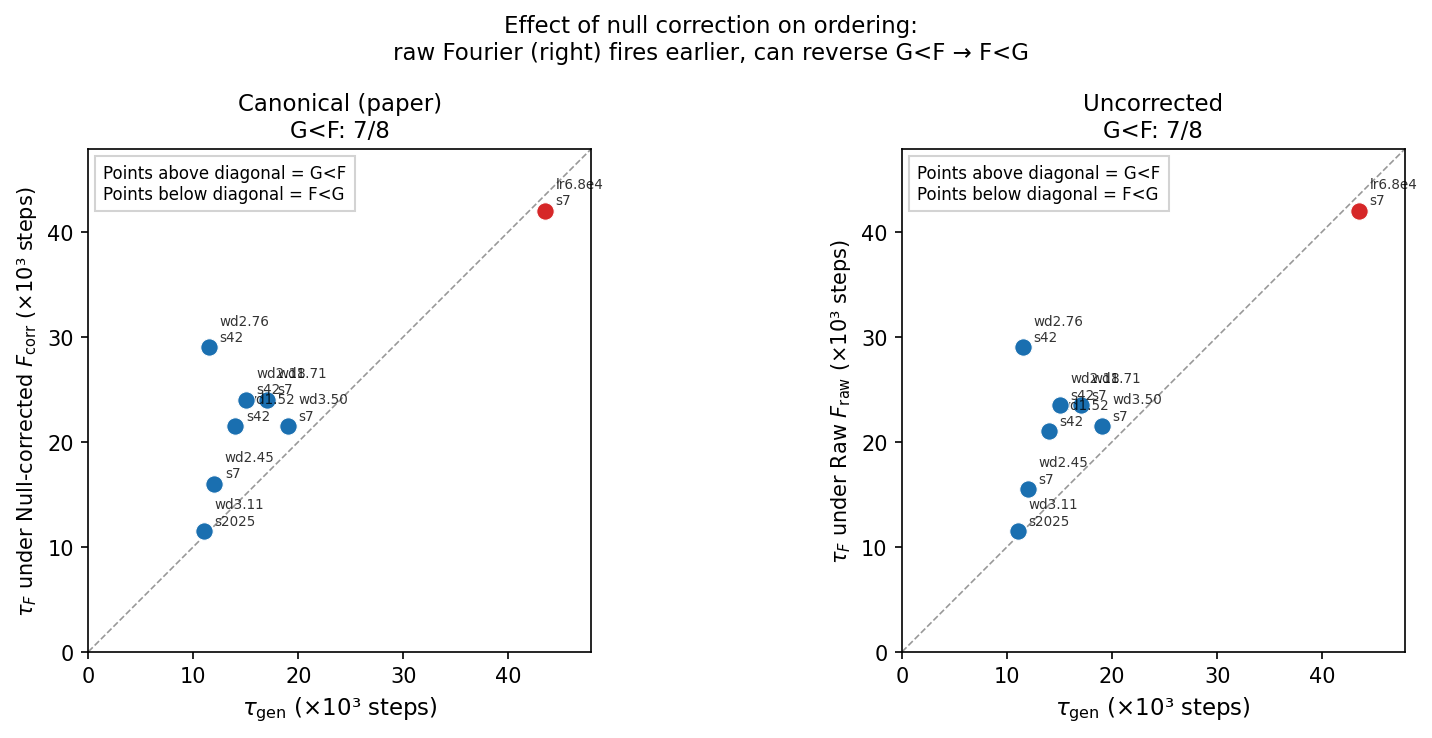
\includegraphics[width=0.85\textwidth]{raw_vs_corr_scatter.png}
\caption{Scatter of $\tauf$ under null-corrected (left) vs.\ raw (right)
  Fourier for 8 sensitivity cells. Points above the diagonal indicate
  G$<$F ordering; points below indicate F$<$G.
  Blue points remain G$<$F under both metrics; the red point (F$<$G
  outlier) remains below the diagonal.
  No ordering flips across the two metrics.}
\label{fig:raw_vs_corr_scatter}
\end{figure}

\subsection{Connection to Superposition and Polysemanticity}
\label{sec:superposition}

The C$<$G$<$F ordering carries a tentative implication for
representation analysis in larger models.
Stage~C ($\taucirc$) marks the BIC-detected onset of
single-harmonic Fourier alignment in the logit space, our
proxy for circuit formation; Stage~F ($\tauf$) marks the later
moment at which the token embedding itself collapses onto the
cyclic-group representation that this proxy already detects in
the logits.
In our 2-layer transformer the two events are separated by
$5{,}000$--$10{,}000$ steps.
The natural reading is that, during the C$<$G window, the network
already implements the correct algorithm but does so on
representations that are still polysemantic: the embeddings
have not yet specialised onto the cyclic-group basis, so the
circuit must operate through a superposition of features rather
than through a clean one-feature-per-direction code.
This is consistent with the broader picture of superposition in
transformers~\citep{elhage2022toy} and with the observation that
monosemantic features can be recovered from polysemantic
activations only with explicit
disentangling~\citep{bricken2023monosemanticity,huben2024sparse}.
Whether an analogue of $\tauf$-style geometry consolidation
appears in larger models is an empirical question we leave open.
The consequence that follows directly from our measurements is
internal: on
this same model, between $\taucirc$ and $\tauf$ the circuit
operates on a representation that the embedding-side metric
$\fcorr$ has not yet identified as cyclic-group-aligned, so
methods that rely on the embedding's geometric handle (linear
probes, dictionary learning) may underdetect the circuit during
that window even though the logit-level Fourier proxy already
flags it.

\subsection{Detector Robustness}
\label{sec:robustness}

A natural concern is whether the G$<$F finding depends on the specific
choice of detector hyperparameters: the null-update interval, the EMA
smoothing coefficient, and the BIC slope threshold.
The null-update interval axis doubles as the artefact check for the
LOCF (piecewise-constant) null schedule introduced in
Section~\ref{sec:methods}: a factor-of-10 change in the refresh
cadence bounds the maximum $\tauf$ displacement that the LOCF
discontinuities could induce.
To address this, 8 cells are selected from the Stage~2$+$3
classification table by a fixed stratification rule---cells
stratified across the measured $|\Dtau|$ distribution (large,
medium, small), plus the coincident cell and the original Stage~3
F$<$G outlier (detector-stable but not replicated under the
cross-hardware re-run of Section~\ref{sec:speed})---and all
$3\times4\times3=36$ detector configurations are
applied post-hoc to the same saved trajectories.
Selecting the subset by a stratification rule applied to the
already-classified table, rather than picking individual cells after
inspecting their detector behaviour, reduces the risk of cherry-picked
robustness.

We define the \textbf{Robustness Score} $\mathrm{RS} = N_{G<F} /
N_{\mathrm{total}}$ for each cell, where $N_{\mathrm{total}}=36$.
Results are shown in Figure~\ref{fig:robustness_heatmap}.
The five cells with $|\Dtau|\geq5{,}000$ steps achieve
$\mathrm{RS}=1.00$ (36/36 configurations yield G$<$F).
The two cells with $|\Dtau|\approx2{,}000$--$3{,}000$ steps achieve
RS$=0.83$ and RS$=0.75$, with the remaining configurations
classifying as \emph{coincident} rather than F$<$G.
Crucially, \textbf{no G$<$F cell is ever classified as F$<$G}
under any configuration.
The mean RS across all seven non-F$<$G cells is \textbf{0.94},
confirming that the G$<$F finding forms a robustness plateau
over the detector parameter space.

\begin{figure}[htbp]
\centering
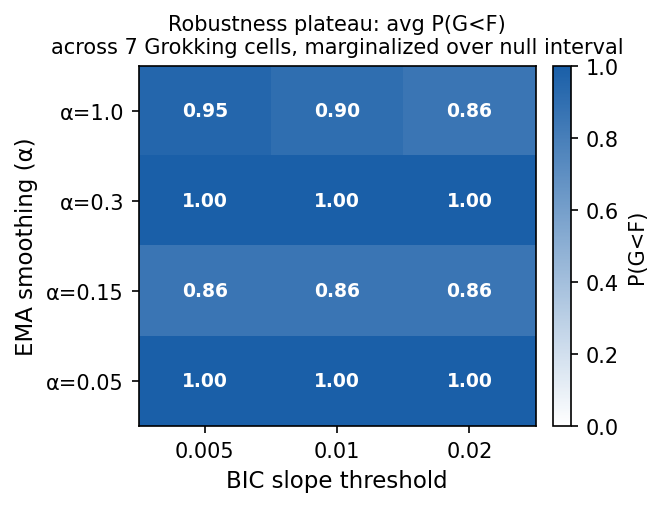
\includegraphics[width=0.52\textwidth]{sensitivity_robustness_heatmap.png}
\caption{%
  \textbf{Robustness plateau.}
  Each cell shows P(G$<$F) for a given (BIC slope threshold, EMA~$\alpha$)
  combination, averaged over null-update intervals \{500, 2500, 5000\}
  and over all seven Grokking cells.
  Strong and medium G$<$F cells achieve 1.00 across all configurations;
  weaker cells ($|\Dtau|\lesssim3{,}000$~steps) degrade gracefully to
  \emph{coincident}, never to F$<$G.
}
\label{fig:robustness_heatmap}
\end{figure}

\paragraph{The two F$<$G cases.}
Both F$<$G runs are real within their original trajectories, and
each has an identifiable origin at the edge of the Grokking phase.

\textit{lr$=6.8\!\times\!10^{-4}$, seed~7} ($\Dtau=-1{,}500$,
RS$=0/36$).
The label is detector-stable: all 36 configurations return F$<$G.
Trajectory inspection locates its origin. $\fcorr$ at $\taug$ is
$0.015$, at the detection floor, while $\taug=43{,}500$
is the latest generalization time in our dataset.
At this very low learning rate, the weight-decay-to-learning-rate
ratio is $\mathrm{wd}/\mathrm{lr}\approx3{,}700$, compared to
$\approx1{,}070$ for a typical G$<$F cell.
The interpretation this supports is that strong relative weight
decay slowly compresses the embeddings toward Fourier-structured
geometry during the long wait before generalization, accumulating
a barely detectable $\fcorr$ signal before the sharp $\taug$
transition, which is the same weight-decay pathway that produces
the lag elsewhere, running at an extreme parameter ratio.
The re-run of this cell on different hardware in the
slow-grokking sweep of Section~\ref{sec:speed} returns
$\Dtau{=}{+}9{,}000$ (G$<$F), placing it within the ordinary
seed-level spread of the main population.

\textit{lr$=4.32\!\times\!10^{-3}$, seed~42} ($\Dtau=-54{,}500$,
RS not assessed).
This is the most extreme case: $\tauf=13{,}000$ but
$\taug=67{,}500$ (extended to 80k steps), with
max\_test\_acc$=0.965$ (below 1.0, indicating incomplete
generalization).
This run sits on the Grokking/Memorization phase boundary and
never completes generalization, so it falls outside the population
the G$<$F claim is about: at high lr the model develops embedding
Fourier structure early while the incomplete generalization
process unfolds on a much longer timescale.

Both cases sit at the edges of the Grokking phase rather than in
its interior, and neither survives as a counterexample: the low-lr
case replicates as G$<$F when re-trained
(Section~\ref{sec:speed}), and the high-lr case does not fully
grok. The targeted slow-grokking sweep of
Section~\ref{sec:speed} tests the phase margin directly, with
$24/24$ purpose-built cells landing G$<$F.

\subsection{Post-hoc Robustness}
\label{sec:posthoc}

The Detector-Robustness analysis above varies the changepoint
pipeline while holding the metric fixed.
This section varies the \emph{metric} while holding the pipeline
fixed, using dense embedding trajectories re-saved from the same
8~sensitivity cells (same (lr,~wd,~seed) combinations and seeds as
Section~\ref{sec:robustness}; embedding matrices recorded every
500~steps, 50{,}000~steps per run).
All eight analyses below are post-hoc and add negligible compute
beyond loading the \texttt{.npz} trajectory files and the
per-run result CSVs (\texttt{results/posthoc/}).

\paragraph{Null threshold and permutation count (\texttt{q2\_null\_sensitivity}).}
We vary the two free parameters of the permutation null: the
percentile $p\in\{90,95,99\}$ and the number of permutations
$n\in\{50,100,200\}$ (9 configurations total).
The canonical detector is $(p{=}95,n{=}100)$.
For each configuration we recompute $F_{\mathrm{null},p}$ at every
log step from the saved embeddings, re-derive $\fcorr$, and re-run
the EMA+BIC changepoint detector.
Table~\ref{tab:q2_null_sensitivity} reports the
per-cell $\Delta\tauf$ relative to canonical.
Across all $8\times9=72$ reconfigurations, $|\Delta\tauf|\leq500$
steps (one log-bin), and for five of the eight cells every one of
the nine configurations returns an identical $\tauf$
($\Delta\tauf=0$).
No cell changes its ordering label under any choice of
$(p,n)$.
This rules out the possibility that the reported G$<$F / F$<$G
labels are artefacts of the canonical $(p_{95},n{=}100)$ null.
\begin{table}[tbp]
  \centering
  \caption{Null-correction sensitivity.
    Per-cell $\Delta\tauf$ (in training steps) across the 9 null
    configurations relative to canonical $(p_{95}, n{=}100)$.
    When the three $n$-values within a percentile column disagree
    we report the full range; ``$0$'' means all three agree with
    canonical.
    Source: \texttt{results/posthoc/q2\_null\_sensitivity.csv}.}
  \label{tab:q2_null_sensitivity}
  \small
  \begin{tabular}{lccc}
    \toprule
    cell (category) & p90 & p95 & p99 \\
    \midrule
    wd1.71\_s7 (strong G$<$F)     & $-500$ & $0$         & $0$            \\
    wd2.76\_s42 (strong G$<$F)    & $0$    & $0$         & $0$            \\
    wd1.52\_s42 (medium G$<$F)    & $0$    & $0,\,+500$  & $+500$         \\
    wd2.18\_s42 (medium G$<$F)    & $-500$ & $-500,\,0$  & $0$            \\
    wd2.45\_s7 (weak G$<$F)       & $0$    & $0$         & $0$            \\
    wd3.50\_s7 (weak G$<$F)       & $0$    & $0$         & $0$            \\
    wd3.11\_s2025 (coincident)    & $0$    & $0$         & $0$            \\
    lr6.8e4\_s7 (F$<$G)           & $0$    & $0$         & $0$            \\
    \bottomrule
  \end{tabular}
\end{table}

\paragraph{Multi-harmonic Fourier variant (\texttt{q3\_multiharmonic}).}
Our canonical $F_{\mathrm{raw}}$ uses $\max_k R^2(E_t\mid\mathrm{span}\,Q_k)$,
which restricts attention to a single harmonic at each step.
A natural generalisation projects onto the top-$K$ harmonics by
per-step energy, yielding $F_K(t)$ with $K\in\{1,2,3,5\}$
($K{=}1$ reproduces the canonical metric as a sanity check).
We recompute the permutation null at matching $K$ (100~shuffles),
re-derive $F_K^{\mathrm{corr}}$, and re-run the changepoint detector.
Table~\ref{tab:q3_multiharmonic} reports $\tauf^K$ and
the resulting ordering label per cell.
Every G$<$F cell retains G$<$F at all four $K$ values
(28/28), and the single F$<$G cell retains F$<$G at all four
(4/4): the ordering is invariant to the harmonic-subspace width.
Contrary to a natural worry, richer subspaces tend to detect
$\tauf^K$ \emph{later}, not earlier, because the top-$K$ subspace
saturates more slowly and the BIC detector demands a correspondingly
larger slope change (seven of eight cells shift by $0$ to
$+6{,}500$ steps between $K{=}1$ and $K{=}5$, and none shift in
the opposite direction beyond $500$).
The single-harmonic metric is therefore, if anything, optimistic
about $\tauf$: widening the subspace only enlarges $\Dtau$ for
G$<$F cells.
\begin{table}[tbp]
  \centering
  \caption{Multi-harmonic $\tauf^K$ and ordering at
    $K\in\{1,2,3,5\}$.
    Every cell preserves its canonical ordering label at all $K$;
    $\tauf^K$ shifts are bounded by $[-1{,}500,\,+6{,}500]$ steps.
    Source: \texttt{results/posthoc/q3\_multiharmonic.csv}.}
  \label{tab:q3_multiharmonic}
  \small
  \begin{tabular}{lccccc}
    \toprule
    cell & $\taug$ & $K{=}1$ & $K{=}2$ & $K{=}3$ & $K{=}5$ \\
    \midrule
    wd1.71\_s7   & $17{,}000$ & $26{,}000$ & $25{,}500$ & $27{,}500$ & $28{,}500$ \\
    wd2.76\_s42  & $11{,}500$ & $30{,}000$ & $30{,}000$ & $30{,}000$ & $30{,}500$ \\
    wd1.52\_s42  & $14{,}000$ & $23{,}000$ & $28{,}000$ & $29{,}000$ & $29{,}500$ \\
    wd2.18\_s42  & $15{,}000$ & $26{,}500$ & $27{,}500$ & $28{,}500$ & $29{,}500$ \\
    wd2.45\_s7   & $12{,}000$ & $18{,}500$ & $17{,}000$ & $16{,}500$ & $18{,}500$ \\
    wd3.50\_s7   & $19{,}000$ & $23{,}000$ & $23{,}000$ & $23{,}500$ & $24{,}500$ \\
    wd3.11\_s2025 & $11{,}000$ & $14{,}000$ & $15{,}500$ & $16{,}500$ & $17{,}500$ \\
    lr6.8e4\_s7 (F$<$G) & $43{,}500$ & $42{,}000$ & $42{,}000$ & $42{,}000$ & $42{,}000$ \\
    \bottomrule
  \end{tabular}
\end{table}

\paragraph{Embedding-layer geometry trajectories (\texttt{q8\_embedding\_geometry}).}
To test whether $\tauf$ coincides with a broader geometric
consolidation, we compute four auxiliary metrics at every
checkpoint:
Frobenius norm $\|E_t\|_F$,
participation ratio
$\mathrm{PR}=(\sum\sigma_i^2)^2 / \sum\sigma_i^4$,
effective rank $e^{S}$ with $S$ the Shannon entropy of the
normalised squared-SV spectrum, and
mean cosine anisotropy
$\mathrm{A}=\mathrm{mean}_{i<j}\,|\cos(E_i,E_j)|$.
For each metric we detect a geometry changepoint $\tau_{\mathrm{geom}}$
via the same EMA+BIC pipeline and compare it run-by-run to $\tauf$.
Table~\ref{tab:q8_geometry} reports the per-cell alignment and
Figure~\ref{fig:q8_geometry_trajectories} overlays the four
trajectories with $\taug$, $\tauf$, and $\tau_{\mathrm{geom}}$
markers on a log-step axis.

\emph{Every one of the $8\times4=32$ (cell, metric) pairs gives
$\tau_{\mathrm{geom}}<\tauf$}, most by a substantial margin.
A consistent temporal ordering emerges within each cell:
$\tau_{\|E\|_F}\!\lesssim\!\tau_{\mathrm{PR}}\!\lesssim\!
\tau_{e^S}\!\lesssim\!\tau_{\mathrm{A}}<\tauf$.
Across cells, median gaps are
$\tauf{-}\tau_{\|E\|_F}\approx 15{,}000$,
$\tauf{-}\tau_{e^S}\approx 13{,}000$,
$\tauf{-}\tau_{\mathrm{A}}\approx 6{,}500$~steps; anisotropy is
the geometry metric closest to $\tauf$, but still precedes it by
more than a log-bin in every cell (minimum gap $1{,}500$ steps).
This falsifies the hypothesis that $\tauf$ is a late readout of
generic embedding-norm or rank growth: Fourier alignment is a
distinct, later event that is \emph{selected from} an already
consolidated geometric substrate.
The same pattern holds for the F$<$G cell (lr6.8e4\_s7): all four
$\tau_{\mathrm{geom}}$ values precede $\tauf$ by
$29{,}500$--$34{,}000$ steps and precede $\taug$ by
$31{,}000$--$35{,}500$ steps, showing that the geometry-first
ordering is not specific to the G$<$F regime.
\begin{table}[tbp]
  \centering
  \caption{Geometry changepoint $\tau_{\mathrm{geom}}$ for
    four embedding-level metrics, compared per cell against
    canonical $\tauf$.
    Every $(cell,metric)$ pair gives $\tau_{\mathrm{geom}}<\tauf$.
    Source: \texttt{results/posthoc/q8\_geometry.csv}.}
  \label{tab:q8_geometry}
  \small
  \begin{tabular}{lcccccc}
    \toprule
    cell & $\taug$ & $\tauf$ & $\|E\|_F$ & PR & $e^S$ & A \\
    \midrule
    wd1.71\_s7    & $17{,}000$ & $25{,}500$ & $10{,}500$ & $14{,}000$ & $15{,}000$ & $22{,}000$ \\
    wd2.76\_s42   & $11{,}500$ & $30{,}000$ & $8{,}000$  & $9{,}000$  & $9{,}500$  & $15{,}500$ \\
    wd1.52\_s42   & $14{,}000$ & $23{,}500$ & $11{,}000$ & $13{,}000$ & $14{,}500$ & $17{,}000$ \\
    wd2.18\_s42   & $15{,}000$ & $26{,}500$ & $9{,}000$  & $10{,}000$ & $11{,}000$ & $15{,}500$ \\
    wd2.45\_s7    & $12{,}000$ & $18{,}500$ & $8{,}000$  & $9{,}500$  & $10{,}500$ & $14{,}000$ \\
    wd3.50\_s7    & $19{,}000$ & $23{,}000$ & $8{,}000$  & $8{,}000$  & $8{,}000$  & $8{,}000$  \\
    wd3.11\_s2025 & $11{,}000$ & $14{,}000$ & $8{,}000$  & $8{,}000$  & $8{,}500$  & $12{,}500$ \\
    lr6.8e4\_s7 (F$<$G) & $43{,}500$ & $42{,}000$ & $8{,}000$ & $9{,}500$ & $10{,}500$ & $12{,}500$ \\
    \bottomrule
  \end{tabular}
\end{table}
\begin{figure}[tbp]
  \centering
  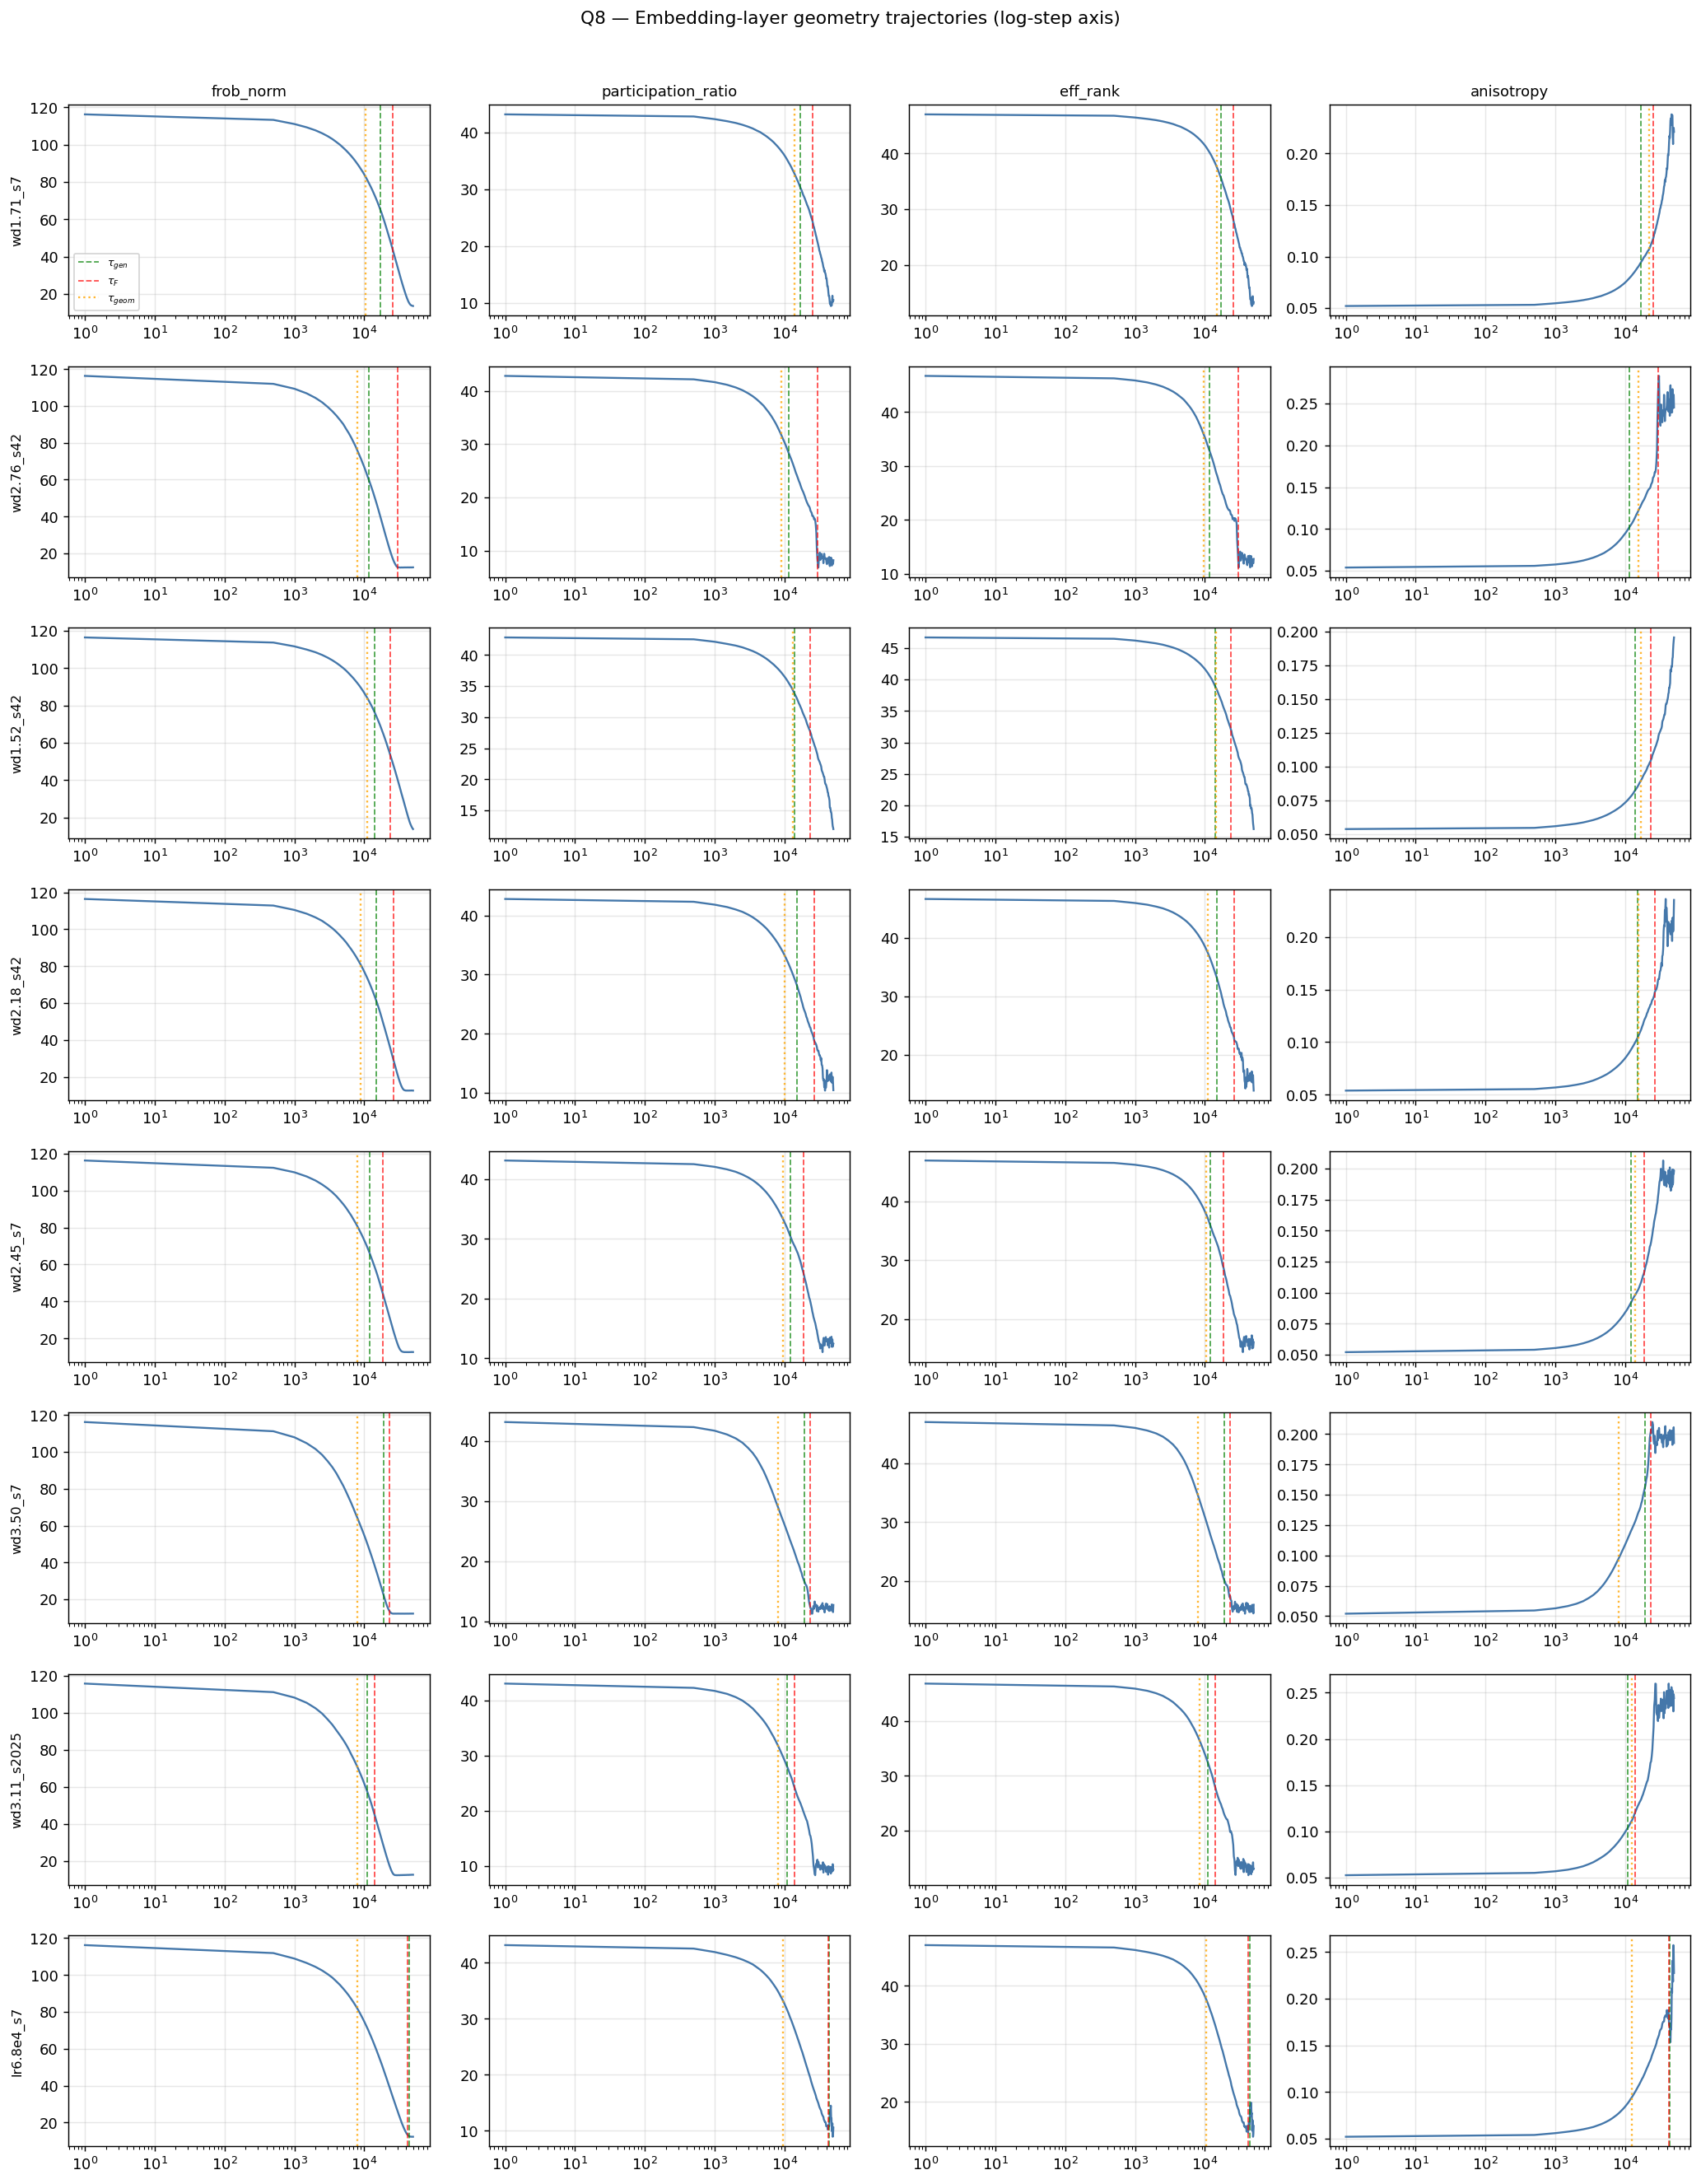
\includegraphics[width=\linewidth]{q8_geometry_trajectories.png}
  \caption{Embedding geometry trajectories.
    Four geometry metrics (columns: $\|E\|_F$, PR, $e^S$,
    anisotropy) for each of the 8 sensitivity cells (rows) on a
    log-step axis.
    Green dashed $=\taug$, red dashed $=\tauf$,
    orange dotted $=\tau_{\mathrm{geom}}$ for the metric shown.
    Every panel has $\tau_{\mathrm{geom}}$ strictly left of
    $\tauf$.}
  \label{fig:q8_geometry_trajectories}
\end{figure}

\paragraph{E6 --- Bootstrap confidence intervals (\texttt{e6\_bootstrap\_ci}).}
To quantify the sampling uncertainty in the headline summaries
used throughout the paper, we run a non-parametric percentile
bootstrap ($n_{\mathrm{boot}}{=}1000$) over the per-run rows of
the five main result CSVs: Stage~2 (wd-sweep at
$\mathrm{lr}{=}1.6{\times}10^{-3}$), Stage~3 (lr-sweep at
$\mathrm{wd}{=}2.5$), Stage~6 (2D $(\mathrm{lr},\mathrm{wd})$
grid), Stage~4 (three-way ordering with $\taucirc$), and E4
(decoupled weight-decay ablation).
$\Dtau$ is computed only where both changepoints are detected;
$\mathrm{P}(\mathrm{G}{<}\mathrm{F})$ is computed over all rows
in each source, so a source containing many memorisation or
F\_only cells naturally reports a lower proportion.
Table~\ref{tab:e6_bootstrap} reports the 95\% CIs, with the
cell-level cluster-bootstrap interval (which keeps all seeds of a
hyperparameter cell together) alongside the row-level interval.
Across the four sweep-type sources the median $\Dtau$ is
strictly positive at the $95\%$ level (lower bound
$\geq 2{,}500$~steps in every case), and
$\mathrm{P}(\mathrm{G}{<}\mathrm{F})$ is bounded away from $0.5$
in each sweep, with the highest-$n$ source (Stage~6, $n{=}147$)
giving the tightest interval $[0.70,\,0.83]$.
E4's lower $\mathrm{P}(\mathrm{G}{<}\mathrm{F}){=}0.43$
$[0.24,\,0.67]$ reflects the by-design presence of non-grokking
ablation cells (the $(0,0)$ and
$(0,\mathrm{wd}^{\star})$ rows of Table~\ref{tab:e4_2x2}); it is
not evidence against G$<$F in the grokking regime.
\begin{table}[tbp]
  \centering
  \caption{E6 --- Non-parametric bootstrap $95\%$ CIs
    ($n_{\mathrm{boot}}{=}1000$).
    $n_{\Dtau}$ is the number of rows with both $\taug$ and
    $\tauf$ detected.
    Median $\Dtau$ and $\mathrm{P}(\mathrm{G}{<}\mathrm{F})$ are
    reported as point estimate with 95\% percentile interval.
    The row-bs column resamples per-run rows as independent units;
    the cluster-bs column resamples (lr, wd) cells with replacement,
    keeping all seeds inside a cell together, and is the
    seed-clustering-aware interval (Table~\ref{tab:cluster_bootstrap}
    gives the full comparison including Stages 5A/5B).
    The Stage~6 cluster estimate is computed over all $147$ rows
    rather than the $126$ detected pairs, hence the $0.75$ vs
    $0.76$ point difference; the cluster bootstrap was not run for
    E4.
    Sources: \texttt{results/posthoc/e6\_bootstrap\_ci.csv},
    \texttt{results/posthoc/cluster\_bootstrap\_ci.csv}.}
  \label{tab:e6_bootstrap}
  \small
  \begin{tabular}{lccccc}
    \toprule
    source & $n$ & $n_{\Dtau}$ & med.\ $\Dtau$ (steps) &
    $\mathrm{P}(\mathrm{G}{<}\mathrm{F})$ row-bs &
    $\mathrm{P}(\mathrm{G}{<}\mathrm{F})$ cluster-bs \\
    \midrule
    Stage~2 (wd)       & $30$  & $30$  & $7{,}750$ $[6{,}000,\,9{,}750]$   & $0.97$ $[0.90,\,1.00]$ & $0.97$ $[0.90,\,1.00]$ \\
    Stage~3 (lr)       & $30$  & $25$  & $4{,}000$ $[2{,}500,\,9{,}500]$   & $0.77$ $[0.60,\,0.90]$ & $0.77$ $[0.57,\,0.97]$ \\
    Stage~6 (2D grid)  & $147$ & $126$ & $6{,}000$ $[5{,}000,\,6{,}500]$   & $0.76$ $[0.70,\,0.83]$ & $0.75$ $[0.66,\,0.84]$ \\
    Stage~4 (circuit)  & $60$  & $54$  & $6{,}000$ $[5{,}000,\,8{,}500]$   & $0.87$ $[0.78,\,0.95]$ & $0.87$ $[0.73,\,0.97]$ \\
    E4 (ablation)      & $21$  & $11$  & $4{,}500$ $[2{,}500,\,10{,}000]$  & $0.43$ $[0.24,\,0.67]$ & --- \\
    \bottomrule
  \end{tabular}
\end{table}

\begin{table}[tbp]
  \centering
  \caption{E6 supplementary --- Per-source comparison of row-level
    bootstrap (Table~\ref{tab:e6_bootstrap}) against a cell-level
    cluster bootstrap that resamples (lr, wd) cells with replacement
    and keeps all seeds inside a cell together
    ($n_{\mathrm{boot}}{=}1000$ each).
    Cluster intervals are 33--40\% wider on the three sources where
    seed clustering is non-degenerate (Stage~3, Stage~6, Stage~4
    retraining); point estimates shift by $<1\%$.
    Stage~2 / Stage~5A / Stage~5B sit at G$<$F rates of
    $97\%$ / $100\%$ / $100\%$ respectively, so intra-cluster variance
    is mechanically near zero and the two bootstraps coincide.
    Source: \texttt{results/posthoc/cluster\_bootstrap\_ci.csv}.
    The Stage~6 row-bootstrap point estimate differs slightly from
    Table~\ref{tab:e6_bootstrap} ($0.75$ vs $0.76$) because this
    table bootstraps all $n{=}147$ rows, while
    Table~\ref{tab:e6_bootstrap} conditions on the
    $n_{\Dtau}{=}126$ rows where both onsets are detected.}
  \label{tab:cluster_bootstrap}
  \small
  \begin{tabular}{lcccc}
    \toprule
    source & $n_{\mathrm{rows}}$ & $n_{\mathrm{cells}}$ &
    $\mathrm{P}(\mathrm{G}{<}\mathrm{F})$ row-bs &
    $\mathrm{P}(\mathrm{G}{<}\mathrm{F})$ cluster-bs \\
    \midrule
    Stage~2 (wd)       & $30$  & $10$ & $0.97$ $[0.90,\,1.00]$ & $0.97$ $[0.90,\,1.00]$ \\
    Stage~3 (lr)       & $30$  & $10$ & $0.77$ $[0.60,\,0.90]$ & $0.77$ $[0.57,\,0.97]$ \\
    Stage~5A (mul)     & $30$  & $10$ & $1.00$ $[1.00,\,1.00]$ & $1.00$ $[1.00,\,1.00]$ \\
    Stage~5B ($p{=}97$)& $30$  & $10$ & $1.00$ $[1.00,\,1.00]$ & $1.00$ $[1.00,\,1.00]$ \\
    Stage~6 (2D grid)  & $147$ & $49$ & $0.75$ $[0.69,\,0.82]$ & $0.75$ $[0.66,\,0.84]$ \\
    Stage~4 (circuit)  & $60$  & $20$ & $0.87$ $[0.78,\,0.95]$ & $0.87$ $[0.73,\,0.97]$ \\
    \bottomrule
  \end{tabular}
\end{table}

\paragraph{E3 --- Comparison with Nanda et al.\ progress measures (\texttt{e3\_nanda\_analysis}).}
A natural concern is that our $\flogit$-based $\taucirc$ might
simply rediscover, in a more elaborate form, what the canonical
restricted-logit and excluded-loss progress measures of
\citet{nanda2023progress} already detect.
We therefore recompute both Nanda metrics on the trajectories of
the $60$ Stage~2$+$3 cells (the same cells used to measure
$\taucirc$ in Section~\ref{sec:results_circuit}; here the
classifier is rerun independently on each trajectory and labels
55 cells Grokking and 5 Memorization, off-by-one from the 54
Grokking runs reported in Section~\ref{sec:results_circuit}
because one borderline cell crosses the sustained-accuracy
threshold under the E3 reclassification but not in the original
Stage~4 pass) and rerun the \emph{same} EMA-smoothed BIC
changepoint pipeline ($\alpha{=}0.15$) on each of the three
scalar series.
Two findings emerge (Table~\ref{tab:e3_nanda}).
First, the \emph{relative} cell-by-cell ordering of the three
detectors is moderately rank-consistent: Spearman $\rho{=}0.54$
($p{=}7.7{\times}10^{-6}$) for excluded loss and $\rho{=}0.42$
($p{=}8.1{\times}10^{-4}$) for restricted loss, both versus our
$\taucirc$ over all 60 paired runs.
The three detectors are therefore \emph{related but not
interchangeable} scalar substitutes for a single underlying
event: the moderate rank agreement is consistent with all three
tracking some aspect of circuit formation, but the rank
correlation is far from unity, so the single-harmonic
$\flogit$ proxy is not a drop-in substitute for a fully
multi-harmonic mechanistic circuit signal.
Second, the \emph{absolute} timing differs systematically:
the median Nanda changepoint lands $2{,}500$~steps later
(excluded) and $4{,}750$~steps later (restricted) than ours, and
agreement to within $\pm 2{,}000$~steps holds in only
$38\%$ and $33\%$ of pairs respectively.
The downstream consequence is the C$<$G rate among the $55$
Grokking-phase runs: our $\flogit$-based $\taucirc$ reports
strict C$<$G in $48/55$ ($87.3\%$) of cells, the excluded-loss
changepoint in $38/55$ ($69.1\%$), and the restricted-loss
changepoint in only $16/55$ ($29.1\%$).
The full three-stage C$<$G$<$F rate falls correspondingly from
$44/55$ ($80.0\%$, ours) to $35/55$ ($63.6\%$, excluded) and
$13/55$ ($23.6\%$, restricted).

\textbf{Reconciling Stage~4's $88.9\%$ with E3's $80.0\%$
(``ours'' detector).}
Stage~4 reports $50/54{=}92.6\%$ C$\leq$G and
$48/54{=}88.9\%$ C$<$G$<$F, while the E3 ``ours'' detector
on the same nominal $60$ (lr, wd, seed) cells gives
$48/55{=}87.3\%$ C$<$G and $44/55{=}80.0\%$ C$<$G$<$F.
The gap is too large for the one-cell phase reclassification
($54$ vs $55$ Grokking).
What actually differs is that Stage~4 and E3 are
\emph{independent training runs} of the same training script with
the same nominal seeds, executed on different GPU/CUDA
configurations (Stage~4 on a local RTX~4080, E3 on a rented A800).
Across the $54$ cells classified as Grokking under both runs, the
per-cell $\tau$ values differ: median $|\Delta\taug|=2{,}000$
steps (90th percentile $7{,}200$, max $30{,}500$), median
$|\Delta\tauf|=3{,}250$, and the three-way ordering label
reclassifies on $8/60$ cells.
We attribute this to non-determinism that survives
\texttt{torch.backends.cudnn.deterministic=True} when sweeps are
run on different GPUs and CUDA versions.
The detector itself ($\flogit$ + EMA + 1-break BIC) is identical
between Stage~4 and E3; the $88.9\%$ vs $80.0\%$ gap is therefore
a measurement of seed-cluster variance under cross-hardware
non-determinism, not a detector disagreement.
We therefore report Stage~4's $48/54$ result as the primary
documented run (it is the configuration described throughout
Sections~\ref{sec:methods}--\ref{sec:results_circuit}) and E3's
$44/55$ result as an independent replication estimate, treating
the C$<$G$<$F rate as a range $[80.0\%,\,88.9\%]$ across two
realizations rather than a single point estimate.

Under a standard EMA+BIC detector, then, the loss-based progress
measures do not yield a clean C$<$G ordering.
Restricted loss inverts the conclusion in three quarters of
grokking cells.
We read this not as a contradiction of Nanda et al., whose
visual analysis already shows early restricted-loss decline, but
as evidence that scalar loss-based progress measures are
\emph{too smooth} for changepoint quantification: the per-step
dynamic-top-$K$ Fourier projection used by $\flogit$ resolves
circuit formation sharply enough that the C$<$G boundary becomes
detector-quantifiable rather than merely eye-visible.
\begin{table}[tbp]
  \centering
  \caption{E3 --- Run-by-run comparison of $\taucirc$ detectors
    on the $60$ Stage~4 runs ($55$ Grokking, $5$ Memorization).
    ``Median $\Delta$'' is the per-pair difference
    (Nanda~$-$~ours) in steps; $|\Delta|{\leq}2{,}000$ is the
    fraction of pairs that agree to within $\pm 2{,}000$~steps;
    Spearman $\rho$ is computed across all $60$ pairs.
    The C$<$G and C$<$G$<$F columns count the $55$
    Grokking-phase runs only.
    Source: \texttt{runs/e3\_nanda/e3\_agreement\_stats.csv} and
    \texttt{results\_e3\_nanda.csv}.}
  \label{tab:e3_nanda}
  \small
  \begin{tabular}{lccccc}
    \toprule
    detector & median $\Delta$ (steps) & $|\Delta|{\leq}2{,}000$ &
    Spearman $\rho$ & $\mathrm{P}(\mathrm{C}{<}\mathrm{G})$ &
    $\mathrm{P}(\mathrm{C}{<}\mathrm{G}{<}\mathrm{F})$ \\
    \midrule
    ours ($\flogit$)        & ---       & ---     & ---                       & $0.873$ ($48/55$) & $0.800$ ($44/55$) \\
    Nanda excluded loss     & $+2{,}500$ & $0.38$ & $0.54$ ($p{=}7.7{\times}10^{-6}$) & $0.691$ ($38/55$) & $0.636$ ($35/55$) \\
    Nanda restricted loss   & $+4{,}750$ & $0.33$ & $0.42$ ($p{=}8.1{\times}10^{-4}$) & $0.291$ ($16/55$) & $0.236$ ($13/55$) \\
    \bottomrule
  \end{tabular}
\end{table}

\paragraph{Detector-specification sensitivity (\texttt{w1\_multibreak\_check}, \texttt{w5\_taugen\_threshold}).}
We add two checks targeting the two specification choices most
likely to be challenged: the 1-break formulation of $\tauf$
and the $0.90$ accuracy threshold of $\taug$.
\textbf{Multi-break check.}
On the same 8 representative cells used elsewhere in
Section~\ref{sec:posthoc}, we refit $\fcorr(\log t)$ with
$0$, $1$, and $2$ breaks and compare BIC.
A 2-break model is BIC-preferred over a 1-break model in 7/8
cells, but the gain comes from adding a \emph{late} second knee
that captures the post-onset saturation plateau (the second break
$\mathrm{bp}_{2}$ falls in $26{,}000$--$42{,}000$~steps, well
after $\taug$); the \emph{early} break $\mathrm{bp}_{1}$ of the
2-break fit lands within median $|\Delta|{=}1{,}500$~steps
(maximum $4{,}000$) of the canonical 1-break $\tauf$.
Read as a sanity check rather than a contradiction: the 1-break
formulation is not hiding a secondary changepoint that would shift
$\tauf$ outside the regime where G$<$F holds; it is collapsing a
smooth two-knee curve into the earlier of its two knees, which is
the timing event of interest.
\textbf{Multi-harmonic and cyclic-group irrep alternatives.}
For $\mathbb{Z}/p$ the non-trivial irreducible representations are
1-dimensional characters whose real-form 2D subspaces coincide with
the Fourier planes used by $F_{\mathrm{raw}}$, so an unrestricted
mean over all $(p{-}1)/2$ irreps is mathematically degenerate
(by Parseval, after centering, it equals the constant $2/(p{-}1)$
at every step).
The closest non-degenerate alternative is to score the sum of the
top-$m$ most-aligned harmonic R$^2$ values, recovering $\tauf^{(m)}$
under the same EMA$+$BIC pipeline.
We recomputed $\tauf^{(m)}$ for $m\in\{1,2,3,5\}$ on the saved
embedding trajectories of the 8 sensitivity cells
(\texttt{src/analysis/multi\_harmonic\_recompute.py}).
$\tauf^{(m)}$ is consistently equal to or later than the canonical
$\tauf^{(1)}$, with median $|\tauf^{(5)} - \tauf^{(1)}| = 2{,}000$
steps and maximum $6{,}500$ steps across the 8 cells; the
single-harmonic detector is therefore the \emph{leading edge}
of the multi-harmonic onset, not a narrower or biased estimate.
The G$<$F ordering label is preserved on all 8 cells under
$m\in\{1,2,3,5\}$, and the $\Dtau$ gap typically widens (e.g.\
wd$=1.52$, seed$=42$ shifts from $\Dtau=9{,}000$ at $m{=}1$ to
$15{,}500$ at $m{=}5$).
A separate $K{=}3$ irrep-mean scoring (an alternative
non-degenerate aggregation) gives the same qualitative result on
the same 8 cells (\texttt{r1\_irrep\_alignment.csv}).
On the logit side, multi-harmonic recompute at the
causal-probe checkpoints (Figure~\ref{fig:causal_intervention})
shows that the top-1 harmonic captures only $10$--$30\%$ of the
logit Fourier energy while the top-5 captures $60$--$85\%$ in the
post-$\taucirc$ regime; this confirms that the full grokked
circuit is multi-harmonic but the single-harmonic onset still
detects the rise correctly.
Extending the same no-break / 1-break / 2-break BIC comparison to
all $60$ Stage~4 $\fcorr$ trajectories plus the $8$ post-hoc
cells ($n{=}68$;
\texttt{results/posthoc/r2\_multibreak\_extended.csv}), $65/68$
cells prefer the 2-break model, but its early break
$\mathrm{bp}_1$ stays within $1{,}500$ steps (3 measurement bins)
of the canonical 1-break $\tauf$ for $30/68$ cells and within
$2{,}500$ steps for $46/68$;
the rare large-displacement cells ($\geq 5{,}500$ steps;
$7/68$) are non-grokking trajectories without a sharply localised
early break, where neither the 1-break nor the 2-break fit has a
well-posed answer.
Across the $8$ headline G$<$F cells, every 2-break fit's early
breakpoint agrees with the 1-break $\tauf$ to within $4{,}000$~steps
and never flips the ordering label.
A future PELT-based analysis on richer trajectories would localise
the saturation knee directly.
\textbf{$\taug$ threshold sweep.}
At thresholds $\theta\in\{0.80, 0.85, 0.90, 0.95\}$ on the same 8
cells (sustained over 3 consecutive 500-step log points), the
median displacement $|\taug(\theta)-\taug(0.90)|$ is $1{,}250$
($\theta{=}0.80$), $750$ ($\theta{=}0.85$), and $750$
($\theta{=}0.95$) steps; the maximum is $9{,}500$ steps at
$\theta{=}0.95$ for one cell whose test accuracy plateau crawls
slowly from $0.90$ to $0.95$.
The typical (median) shift is well below the median
$\Dtau{=}6{,}000$~steps of cells with $|\Dtau|\geq3{,}000$
(Section~\ref{sec:posthoc}), so the G$<$F ordering at the level of
headline 95\% CIs is insensitive to the threshold choice across
$[0.80,0.95]$.
The single 9{,}500-step worst case occurs because the run's test
accuracy plateau crawls slowly between $0.90$ and $0.95$, which
is precisely the regime where any $\taug$ definition becomes
fragile; near-coincident cells ($|\Dtau|\leq 2{,}000$) cannot be
reliably classified at \emph{any} threshold and are already
excluded by the measurement-resolution caveat in
Section~\ref{sec:limitations}.
Full per-cell tables are in
\texttt{results/posthoc/w1\_multibreak.csv} and
\texttt{w5\_taugen\_threshold.csv}.

\paragraph{E7 --- Causal Fourier-subspace intervention.}
Timing alone cannot say whether the subspace our detector tracks
does any work.
To test whether the dominant low-order Fourier subspace
identified by the proxy is causally load-bearing rather than a
correlated readout, we probe twelve cells: five original cells
spanning the phase diagram (strong C$<$G$<$F, G$<$C$<$F boundary,
C$<$F$<$G slow-grokking, canonical, coincident) plus seven
expansion cells varying seed ($\times 2$), weight decay
($\times 2$), learning rate ($\times 1$), task (multiplication,
$\times 1$), and prime ($p{=}97$, $\times 1$).
Each cell is saved at three to four regime-boundary checkpoints
(pre-all, between events, post-all).
At each checkpoint we apply four interventions on the trained
logits: \textbf{(I1)} keep only the top-$3$ Fourier harmonics of
the output-class index, \textbf{(I2)} remove them, \textbf{(I3)}
remove a matched-energy random subspace as control, and
\textbf{(I4)} apply the same Fourier removal to the token
embedding rows (anonymised supplementary code).
All four are representation-space projections evaluated at frozen
checkpoints: I1--I3 act on the trained logit matrix with a basis
indexed by the answer class, and I4 acts on the embedding rows
with a basis indexed by the token value.
They answer whether the projected subspace is necessary for test
accuracy at a given step; the complementary question of
\emph{where} in the network that structure is computed is
answered by the label-free internal patch reported at the end of
this subsection, whose random control is dimension-matched in the
same way as I3.

Four findings emerge (Figure~\ref{fig:causal_intervention}
shows a five-cell subset).
First, on the eight addition-mod-53 cells that fully grok,
the maximum I2 drop across between-event checkpoints reaches
$0.40$--$0.72$ in absolute test accuracy (specificity
$12$--$214\times$ over matched-energy random controls),
demonstrating that the top-$3$ Fourier subspace is causally
load-bearing.
The effect extends to $p{=}97$: top-3 alone is insufficient
(I2 drop $0.004$) because the larger prime spreads load across
more harmonics, but at $K{=}5$ the drop reaches $0.38$ and at
$K{=}10$ it reaches $1.00$, all with random-control drops of
exactly $0.000$.
The multiplication cell (\texttt{mul\_GF}) gives a clean negative
that is informative in its own right: specificity ${\approx}1\times$
at every $K$, and the internal patch below reproduces the same
null at every site.
Multiplication is reindexed through a discrete logarithm, so the
cyclic-group harmonics that carry load for addition are not the
directions the network uses, even though its \emph{timing}
behaviour is indistinguishable from addition ($30/30$ G$<$F in
Stage~5A).
This separates the two scopes cleanly: the embedding-ring lag is
a timing regularity that transfers across the tasks we tested,
while the identification of \emph{which} subspace bears load is
task-specific and holds where the cyclic-group basis is the
operative one (addition mod $53$ and mod $97$).
Headline intervention statistics are quoted over the
addition cells accordingly.
The remaining cell that does not fully grok (\texttt{FG\_slow},
max test accuracy $0.51$) shows correspondingly smaller but still
positive I2 effects ($0.02$--$0.39$); we include it in
Figure~\ref{fig:causal_intervention} for completeness.
Second, after $\tauf$ the I2 drop on logits collapses while I4
on embeddings stays large, a pattern consistent with
redistribution of the answer across the logit representation
after $\tauf$ while the embedding remains Fourier-dependent.
Third, the G$<$C$<$F cell (\texttt{G\_CF\_boundary},
$\taug{=}6{,}500<\taucirc{=}8{,}000$) shows Fourier load-bearing
already at step $7{,}000$ (drop $0.69$, specificity $112\times$),
reframing the four G$<$C$<$F exceptions in
Section~\ref{sec:results_circuit} as detector-resolution artefacts.
Fourth, I4 is not inert before $\tauf$: at checkpoints between
$\taug$ and $\tauf$ on the same eight
fully-grokking addition cells, removing the top-$3$ Fourier
directions from the token embedding reduces test accuracy from
a baseline of $0.90$--$1.00$ to $0.02$--$0.37$
(\texttt{results/causal\_probe\_combined/intervention\_results.csv}).
Embedding Fourier \emph{content} is therefore functionally
necessary well before the BIC-detected consolidation at $\tauf$.
This sharpens rather than contradicts the dissociation: what lags
generalization is the consolidated global geometry that $\fcorr$
(and a PCA ring plot) detects, not the first functional presence
of Fourier structure in the embedding.
$\tauf$ should accordingly be read throughout as a
\emph{consolidation changepoint} rather than a first-appearance
time, and the headline claim concerns the late consolidation of
the visible ring, not causal irrelevance of the embedding before
$\tauf$.

\paragraph{Why $K{=}3$? A top-$K$ ablation spectrum.}
A reasonable concern is whether $K{=}3$ is privileged or whether
removing any low-rank subspace would damage accuracy similarly.
We rerun the intervention for $K\in\{1,3,5,10\}$ on all twelve
cells, using the same matched-energy random-subspace control at
each $K$.
Table~\ref{tab:topk_spectrum} reports medians over the fifteen
between-events checkpoints with base accuracy $>0.5$ (excluding
\texttt{mul\_GF}).
The causal effect grows smoothly with $K$ from $K{=}1$ (insufficient
coverage; I2 drop $0.080$) through $K{=}3$ (drop $0.551$) to
$K{=}5$ (drop $0.812$), and saturates by $K{=}10$ (drop $0.974$).
At every $K$ the matched-energy random control remains within
$|\Delta\,\mathrm{acc}|\leq 0.007$ of unintervened accuracy, so the
specificity of top-$K$ Fourier removal over a random subspace
\emph{rises} from $10{\times}$ ($K{=}1$) to $\geq 360{\times}$
($K{=}5$).
The shape of the curve confirms that the causal effect is
localized to low-order logit-Fourier structure rather than to
arbitrary low-rank damage.

\begin{table}[!ht]
  \centering
  \small
  \caption{Top-$K$ ablation spectrum on the twelve causal-probe
    cells (excluding \texttt{mul\_GF}), restricted to between-events
    checkpoints with base accuracy~$>0.5$ ($n{=}15$). I2 removes
    the top-$K$ Fourier harmonics; I3 removes a matched-energy
    random subspace. Specificity is I2 drop / I3 drop.}
  \label{tab:topk_spectrum}
  \begin{tabular}{rrrr}
    \toprule
    $K$ & median I2 drop & median I3 ctrl drop & median specificity \\
    \midrule
    1   & $+0.080$ & $+0.007$ & $10.4\times$ \\
    3   & $+0.551$ & $+0.005$ & $37.5\times$ \\
    5   & $+0.812$ & $+0.001$ & $362\times$ \\
    10  & $+0.974$ & $-0.004$ & (saturated)\textsuperscript{\dag} \\
    \bottomrule
  \end{tabular}\\[2pt]
  \footnotesize\textsuperscript{\dag}At $K{=}10$ the random control
  drop is slightly negative on the median, making the specificity
  ratio undefined; I2 drop has saturated near $1.0$ regardless.
\end{table}

\paragraph{Are the top-$K$ harmonics special, or would any $K$ Fourier directions do? A frequency-selectivity control.}
The top-$K$ subspace removal still leaves open a second attack: maybe
the load-bearing structure is just ``any $K$ Fourier directions'',
not specifically the high-power ones. We test this directly by
comparing, at the same checkpoints and at $K{=}3$, three alternative
ablations that stay \emph{inside} the Fourier basis but pick
different frequencies:
\textbf{top-3} (the three harmonics with the highest centered-logit
power, the canonical I2),
\textbf{alt-3} (three harmonics drawn uniformly from rank
$\geq 10$, averaged over 5 random draws), and
\textbf{bot-3} (the three lowest-power harmonics).
For comparison we also report the matched-energy non-Fourier
random-subspace control (I3) used throughout this section.
Table~\ref{tab:freq_selectivity} summarises the result over the
fifteen between-events checkpoints (excluding \texttt{mul\_GF}).
Top-3 removal drops accuracy by a median of $0.55$; alt-3 and
bot-3 removals drop accuracy by $-0.003$ and $-0.002$ on the
median, statistically indistinguishable from the matched-energy
non-Fourier random control ($+0.008$).
The load-bearing logit-Fourier structure is therefore not ``any
$K$ Fourier directions'' but specifically the small set of
high-power answer-class harmonics.

\begin{table}[!ht]
  \centering
  \small
  \caption{Frequency-selectivity control at $K{=}3$ on twelve
    causal-probe cells (excluding \texttt{mul\_GF}), restricted to
    between-events checkpoints with base accuracy~$>0.5$ ($n{=}15$).
    Every variant removes a 3-harmonic Fourier subspace from the
    centered logits; they differ only in \emph{which} three
    harmonics are chosen.}
  \label{tab:freq_selectivity}
  \begin{tabular}{lr}
    \toprule
    Removed subspace ($K{=}3$) & median accuracy drop \\
    \midrule
    top-3 Fourier (by power) & $+0.551$ \\
    alt-3 Fourier (rank $\geq 10$, mean of 5 random draws) & $-0.003$ \\
    bot-3 Fourier (lowest-power) & $-0.002$ \\
    matched-energy non-Fourier random subspace (I3) & $+0.008$ \\
    \bottomrule
  \end{tabular}
\end{table}

\begin{figure}[!tbp]
  \centering
  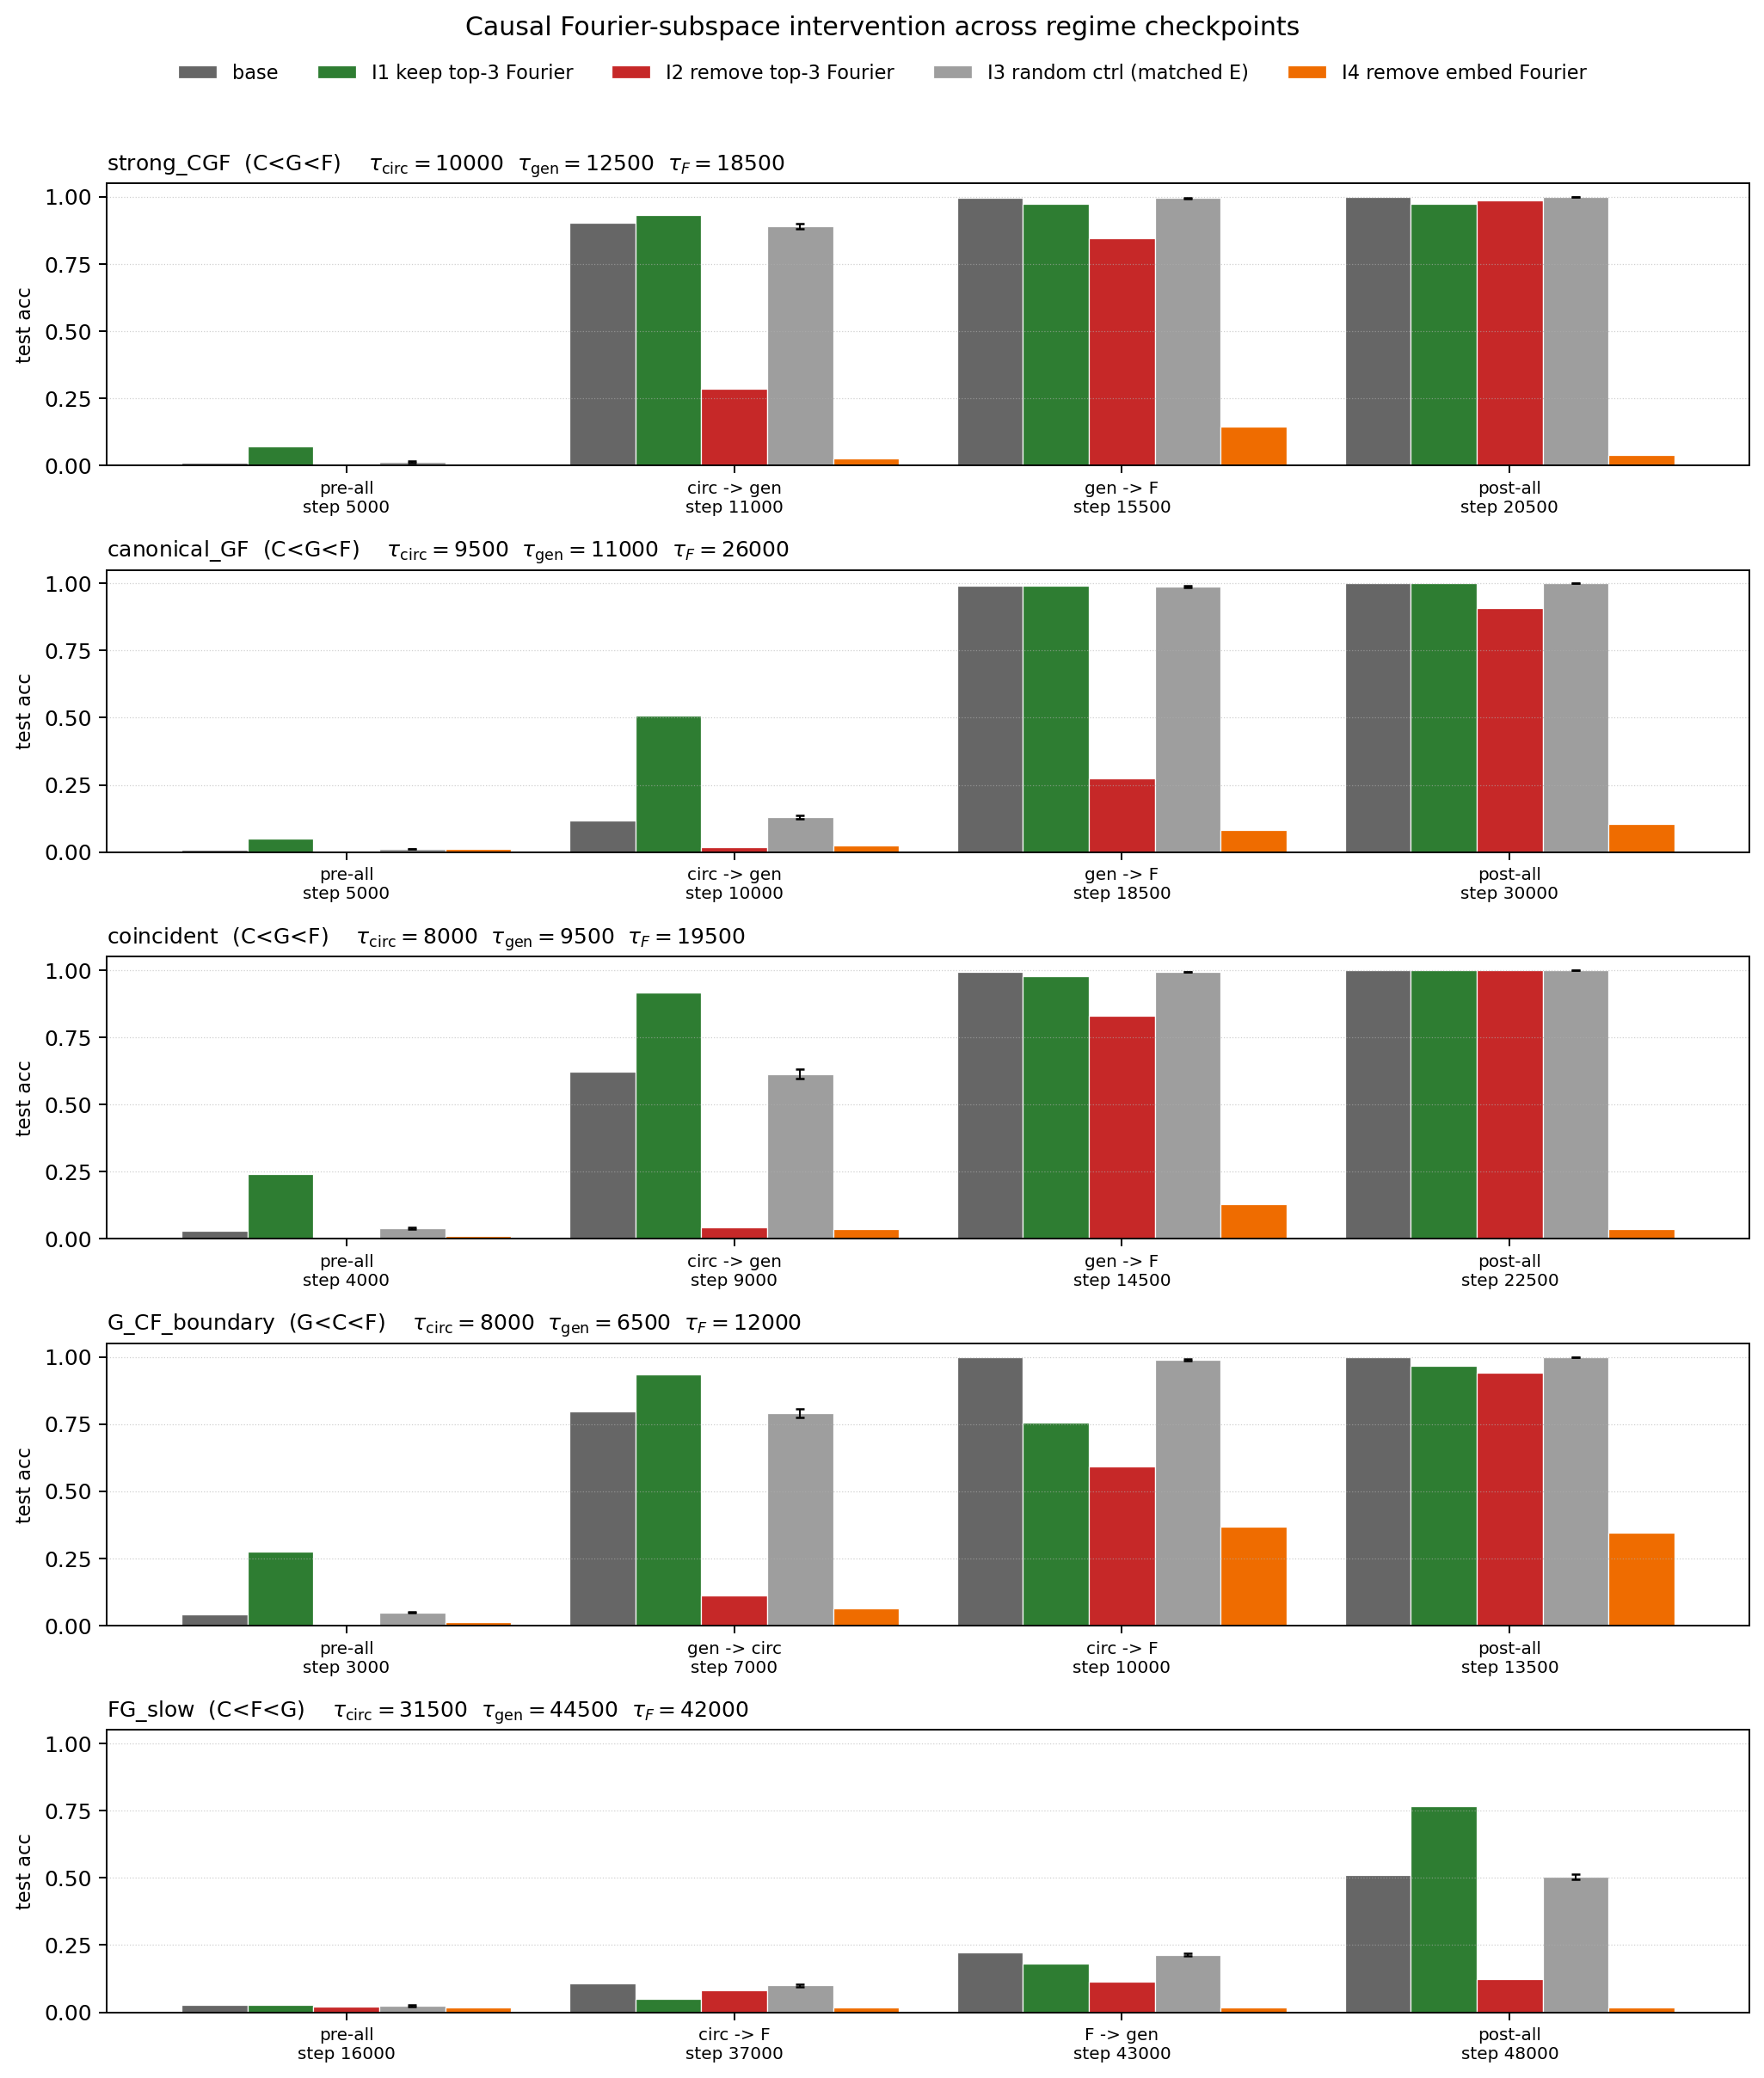
\includegraphics[width=0.92\linewidth]{causal_intervention_grid.png}
  \caption{%
    \textbf{Causal Fourier-subspace intervention (five-cell subset
    of the twelve probed cells).}
    Each row is one cell; the four bar groups are regime checkpoints
    (\textit{pre-all}, between-event, \textit{post-all}); each
    group reports test accuracy under five conditions:
    unintervened \texttt{base}; \texttt{I1}~keep only the top-$3$
    Fourier harmonics; \texttt{I2}~remove them; \texttt{I3}~a
    matched-energy random-subspace control;
    \texttt{I4}~remove top-$3$ Fourier from the token embedding.
    The large I2 drops with negligible I3 effect in the
    between-event regime (specificity $12$--$214\times$ across all
    eight fully-grokked addition-mod-53 cells) establish the
    dominant answer-aligned Fourier subspace as functionally
    necessary.
    Note that I4 (orange) is already large at between-event
    checkpoints: embedding Fourier content is functionally
    necessary before $\tauf$ (see text).
    The post-$\tauf$ I2 collapse alongside the sustained I4 drop
    is consistent with redistribution or redundancy in the logit
    representation after $\tauf$, while the embedding remains
    Fourier-dependent.
  }
  \label{fig:causal_intervention}
\end{figure}

\paragraph{Internal activation patching (F4 pilot).}
To address the offline output-space scope of I1--I4, we also ran a
\emph{label-free, component-level} pilot on the same 43 probe
checkpoints (script
\texttt{src/analysis/activation\_patching\_probe.py}, results
\texttt{results/activation\_patching/}).
At six internal sites (embedding output, per-layer attention and
MLP outputs, final residual stream) we view each activation channel
as a function on the $(a,b)$ input grid, ablate the top-$3$
grid-Fourier harmonics selected by activation power (no ground-truth
label enters the construction), and compare against a
dimension-matched random-subspace control mirroring I3
(5 draws per site).
On the ten between-event ($\taug{<}t{<}\tauf$) addition-mod-53
checkpoints with base accuracy above $0.5$, ablation at the final
residual stream drops test accuracy by a median of $0.49$ while the
random control drops it by $0.02$; the second-layer MLP output
(\texttt{mlp\_L1}) shows
drops of $0.66$ vs $0.10$, and second-layer attention
(\texttt{attn\_L1}) $0.77$ vs $0.21$.
On the $p{=}97$ cell the separation is sharper still (residual
stream $0.44$ vs $0.00$), and the multiplication cell replicates
the E7 negative (ablation ${\approx}$ control at every site).
The grid-space control is the informative comparison at the four
sites whose activations mix both input tokens.
At the embedding output and the first-layer MLP output
(\texttt{mlp\_L0}), activations are (partially) separable
functions of a single token, so a random grid-space direction
moves them off the low-dimensional manifold the network ever
produces while the axis-aligned Fourier ablation stays on it;
the embedding side is accordingly read from I4, whose basis
respects that structure.
The pilot localizes Fourier-specific functional necessity to the
second-layer components and the final residual stream during the
$\taug$--$\tauf$ window, adding an internal, label-free probe to
the output-space interventions
(Appendix~\ref{app:future_work}, F4).

The eight post-hoc analyses above, together with the detector
sensitivity in Section~\ref{sec:robustness}, show that the
three-stage ordering survives changes to the null-correction
parameters, multi-harmonic Fourier variants, idle-step
interpolation choices, embedding-geometry definitions,
bootstrap sampling uncertainty, the choice of progress measure
used to locate $\taucirc$, the canonical 1-break formulation of
$\tauf$ versus the post-hoc 2-break sanity check, and the
accuracy threshold used to define $\taug$.
All source scripts and expected artefacts are listed in
Appendix~\ref{app:details} (``Release plan'').

\subsection{Limitations}
\label{sec:limitations}

\paragraph{Task scope.}
Our three-stage confirmation covers $(a+b)\bmod p$ and $(a\cdot b)\bmod 53$.
Stage~5B extends to $p{=}97$.
Generalization to non-modular tasks or non-algorithmic settings
remains open.

\paragraph{Architecture scope.}
All main experiments use the same 2-layer transformer.
A small post-hoc depth pilot at the canonical operating point
shows that the ordering does not transfer automatically:
$n_{\mathrm{layers}}{=}1$ gives F${<}$G in 3/3 seeds, and
$n_{\mathrm{layers}}{=}3$ gives F${<}$G in 2/3 seeds
(Appendix, F2).
One plausible account is that deeper networks provide alternative
pathways that let logit-Fourier structure propagate into embeddings
before generalization, collapsing the timing gap.
Because this pilot covers only one operating point and two depths,
we treat it as a scope warning; a systematic depth$\times$width
transfer study remains the primary future work.

\paragraph{Measurement resolution.}
$\Dtau$ is measured with 500-step resolution;
small lags ($|\Dtau|\lesssim500$) cannot be reliably classified.
One F$<$G run has $|\Dtau|=1{,}500$ (three log-intervals),
above the resolution floor but warranting caution.

\paragraph{Intervention controls.}
The logit-side interventions (I2) and the internal activation
patch are each paired with a dimension-matched random-subspace
control, and both report specificity against that control.
The embedding-side intervention I4 is reported without such a
pairing: at the embedding and first-layer sites the activations
are (partially) separable functions of a single input token, and
a random direction drawn in grid-function space moves them off
that low-dimensional manifold, so a random control there measures
manifold departure rather than Fourier specificity.
I4 should accordingly be read as establishing that embedding
Fourier content is functionally in use, without a specificity
ratio attached; designing on-manifold controls for these sites is
part of the systematic study in
Appendix~\ref{app:future_work}, F4.

\paragraph{Logit metric alignment.}
Our $\flogit$ captures the aggregate Fourier structure of logits
across all $(a,b)$ pairs, which is related but not identical to
Nanda et al.'s restricted logit loss.
A direct comparison on the same 60 Stage~2$+$3 runs (E3,
Section~\ref{sec:posthoc}, Table~\ref{tab:e3_nanda}) shows
moderate rank agreement (Spearman $\rho{=}0.42$--$0.54$),
confirming that the three detectors track related but not
interchangeable aspects of circuit formation.

\paragraph{Phase-boundary regime.}
The 4~G$<$C$<$F exceptions in Stage~4 all occur at high lr
where generalization is very fast and the BIC changepoint may
underestimate $\taucirc$ when the logit signal rises gradually
rather than sharply.
The causal Fourier-subspace intervention E7
(Section~\ref{sec:posthoc}, Figure~\ref{fig:causal_intervention})
supports this detector-lag interpretation on one representative
high-lr G$<$C$<$F cell, where the dominant Fourier subspace is
already causally load-bearing at step~$7{,}000$ even though the
BIC-detected $\taucirc$ lands at step~$8{,}000$;
we have not, however, intervened on all four exceptions, so we
treat the detector-lag explanation as supported but not
exhaustively verified.

\paragraph{Cyclic-group structural assumption.}
The $\fcorr$ detector projects the embedding matrix onto the
2-dimensional Fourier subspaces of the cyclic group $\mathbb{Z}/p$
and the $a\cdot b\bmod p$ extension uses a discrete-log reindexing
to the same cyclic-group target.
Algorithmic variants that solve modular arithmetic via non-cyclic
representations (for example, factor-group decompositions on
composite moduli, or learnt non-Fourier features) would not
register on $\fcorr$ in its present form, and the
$\taucirc<\taug<\tauf$ claim should be read as conditional on the
cyclic-group structural prior.

\paragraph{Residual structure and bootstrap independence.}
The BIC changepoint estimator assumes i.i.d.\ Gaussian residuals on
the log-time axis and the bootstrap CI in
Table~\ref{tab:e6_bootstrap} resamples per-run rows as i.i.d.\
units.
The reported intervals should therefore be read as descriptive
row-level bootstrap intervals rather than fully valid confidence
intervals under clustered dependence across hyperparameter cells:
seed-level dependence within a cell is not accounted for by
independent-row resampling and may either inflate or deflate the
apparent variance.
We quantify this gap with a per-source cell-level cluster
bootstrap that resamples (lr, wd) cells with replacement and
keeps all seeds inside a cell together
(Table~\ref{tab:cluster_bootstrap};
\texttt{src/analysis/cluster\_bootstrap.py}).
On the three sources where seed clustering is non-degenerate
(Stage~3, Stage~6, Stage~4 retraining), the cluster-bootstrap
$95\%$ CI for $\mathrm{P}(\mathrm{G}{<}\mathrm{F})$ is $33$--$40\%$
wider than the row-bootstrap CI; the headline point estimates
shift by $<1\%$.
We position this comparison as a descriptive bootstrap-uncertainty
diagnostic rather than a cluster-robust inferential replacement;
Table~\ref{tab:e6_bootstrap} reports the cluster-bootstrap
interval alongside the row-level interval for each source, and
the Wilson intervals in Table~\ref{tab:summary_all} remain
run-level and carry the same caveat.
The row-bootstrap intervals are mildly anti-conservative but not
qualitatively misleading; where seed clustering matters, the
cluster-bootstrap interval is $\sim$$33$--$40\%$ wider.
Stage~5A, Stage~5B and Stage~2 are at $\mathrm{P}(\mathrm{G}{<}\mathrm{F})$
rates of $100\%$, $100\%$ and $96.7\%$ respectively, so
intra-cluster variance is mechanically near zero and the two
bootstrap variants coincide.
Heteroscedasticity in $\fcorr$ residuals is not formally tested.

\paragraph{Detector-specification scope.}
The robustness sweeps in Section~\ref{sec:robustness} and
Section~\ref{sec:posthoc} vary the detector along axes we
identified ahead of time (EMA $\alpha$, BIC slope threshold, null
refresh interval, $\taug$ threshold, canonical 1-break formulation versus post-hoc 2-break sanity check).
Adversarial detector specifications outside this grid are not
ruled out, and an alternative onset definition that rejects
single-harmonic projection altogether (for example, group-irrep
based detectors) could in principle reorder $\taucirc$ and $\tauf$.

% ==============================================================
\section{Ruling Out a Speed-Dependent Explanation of the Ordering}
\label{sec:speed}

The single strongest alternative account of our result is that
G$<$F is not a property of how representations form at all, but an
artefact of \emph{how fast} the network generalises: if embedding
consolidation runs on its own clock, then fast grokking would
simply beat that clock and slow grokking would lose to it.
This section states that account precisely and tests it directly,
using a data-subsampling speed control (E5,
Section~\ref{sec:e5_subsample}), a targeted sweep engineered to
enter the regime where the account predicts a reversal, and a
leave-one-out predictive diagnostic on the Stage~6 grid.
Inside the regime it nominates as decisive, the account's
prediction does not hold.

\paragraph{The account, stated precisely.}
Let $\taug$ and $\tauf$ be determined by two largely separable
processes: generalization by the dynamics of the circuit that
solves the task, and embedding-geometry consolidation by the
indirect reshaping of the embedding rows through gradients
back-propagated from the regularised decoder (recall that in our
setting $\mathrm{wd}_{\mathrm{emb}}{=}0$, so the embedding has no
direct $L_2$ pressure and is shaped only via the decoder's
weight-decay clock).
If these two processes run on roughly parallel clocks, the observed
ordering becomes a function of generalization speed:
\begin{itemize}
  \item when $\taug$ is small (``fast grokking''), generalization
    fires before the embedding geometry has had time to consolidate,
    yielding G$<$F;
  \item when $\taug$ is large (``slow grokking''), weight decay has
    enough time to complete embedding consolidation first, yielding
    F$<$G.
\end{itemize}
This picture is compatible with \citet{doshi2024grok}, who show that
on corrupted modular-arithmetic data the relative onsets of
memorization and generalization depend separately on data corruption,
weight decay, and learning rate; and with the implicit-bias view in
which weight decay continues to restructure representations long
after the training loss has saturated \citep{soudry2018implicit,
galanti2024sgd,andriushchenko2023need}.

\paragraph{Evidence from existing data.}
Three observations in our dataset are consistent with this hypothesis.

\emph{(i) Location of F$<$G exceptions.}
Both F$<$G runs in the 1D sweeps occur at the margins of the Grokking
phase where $\taug$ is unusually late: $\taug{=}43{,}500$~steps
(lr$=6.8\!\times\!10^{-4}$, seed~7; $\Dtau=-1{,}500$) and
$\taug{=}67{,}500$~steps (lr$=4.32\!\times\!10^{-3}$, seed~42;
$\Dtau=-54{,}500$, max test accuracy 0.965).
In Stage~6, 11 of 13 F$<$G cases lie on the outermost lr rows of
the 2D grid, consistent with the same pattern.

\emph{(ii) Cross-task pilot.}
A pilot run of modular \emph{subtraction} $(a{-}b)\bmod 53$ at the
same hyperparameters as our Stage~2 core cell
(wd$=2.18$, lr$=1.6\!\times\!10^{-3}$) groks much later than addition
($\taug{=}43{,}500$~steps vs $\approx 11{,}000$~steps for addition)
and lands in the F$<$G regime ($\Dtau{=}{-}9{,}000$).
A second subtraction seed at the same hyperparameters groks faster
($\taug{=}27{,}500$~steps) and returns to G$<$F ($\Dtau{=}{+}5{,}500$),
providing \emph{within-task, within-hyperparameter} evidence that
the ordering flip tracks generalization speed rather than task
identity.

\emph{(iii) Aggregate correlation.}
Across 57 Grokking runs (55 addition + 2 subtraction pilots),
$\Dtau$ and $\taug$ are negatively correlated ($r=-0.62$;
Figure~\ref{fig:speed_ordering}).
All F$<$G runs have $\taug\geq 43{,}000$~steps; the majority of
G$<$F runs have $\taug\leq 35{,}000$~steps.
Because $\Dtau=\tauf-\taug$ is defined relative to $\taug$, part of
this correlation is mechanical and should not be interpreted
causally on its own; the within-task seed comparison in~(ii)
is free of this confound and is what load-bears the hypothesis.

\begin{figure}[htbp]
  \centering
  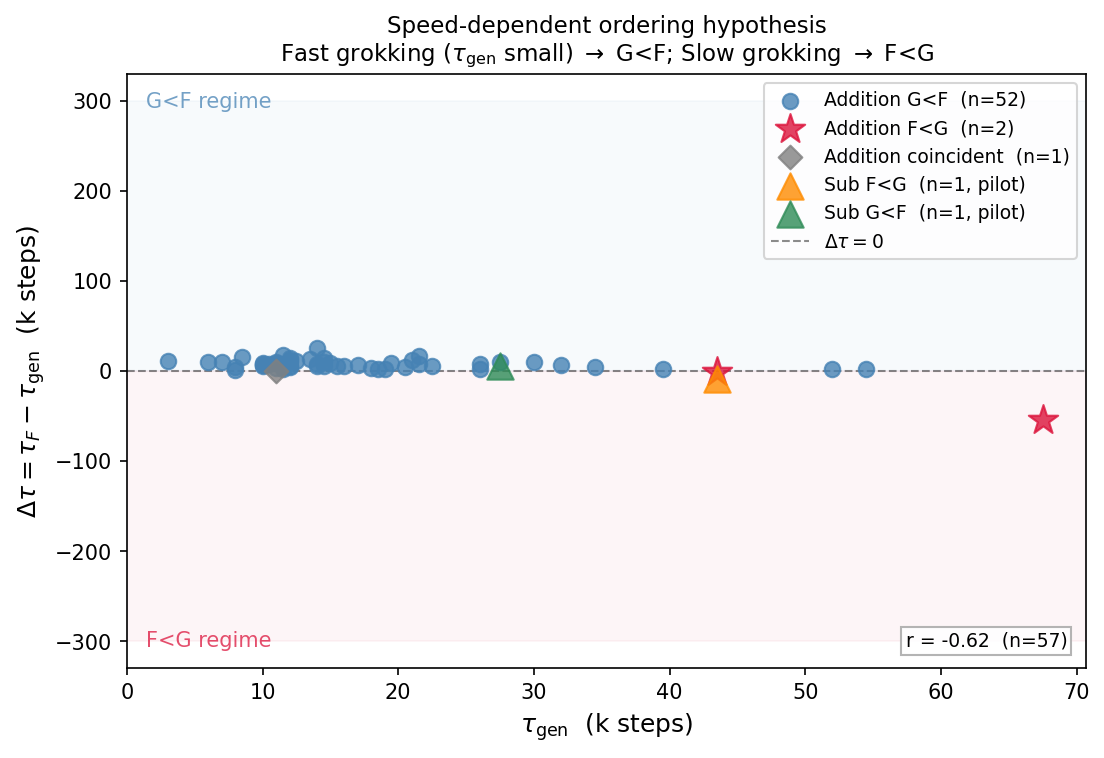
\includegraphics[width=0.80\linewidth]{speed_ordering_scatter.png}
  \caption{%
    \textbf{Speed-dependent ordering.}
    Scatter of generalization onset $\taug$ vs lag $\Dtau{=}\tauf{-}\taug$
    for all 55 Grokking addition runs (blue circles = G$<$F, red stars
    = F$<$G, grey diamond = coincident) and 2 subtraction pilots
    (orange triangles; 1 F$<$G, 1 G$<$F).
    All F$<$G runs cluster at $\taug\geq43{,}000$~steps;
    overall $r{=}{-}0.62$ ($n{=}57$).
    The two subtraction pilots at identical hyperparameters (wd$=2.18$,
    lr$=1.6\!\times\!10^{-3}$) differ only in seed and generalization
    speed, yet flip ordering---within-task evidence that the effect
    is not a pure $\Dtau=\tauf-\taug$ construction artefact.
  }
  \label{fig:speed_ordering}
\end{figure}

\paragraph{Leave-one-out predictive diagnostic.}
A leave-one-out logistic regression on the 123 Stage~6 cells with
both $\taug$ and $\tauf$ detected and $|\Dtau|>500$, using
$(\log_{10}\mathrm{lr}, \log_{10}\mathrm{wd}, \log(1+\taug))$ as
features and binary $\mathrm{sign}(\Dtau)$ as target, achieves
ROC-AUC $0.945$ ($95\%$ bootstrap CI $[0.896, 0.981]$,
$n_{\mathrm{boot}}{=}1000$); restricting the model to
$(\log_{10}\mathrm{lr}, \log_{10}\mathrm{wd})$ alone drops AUC to
$0.549$, while $\log(1+\taug)$ alone retains $0.925$.
We frame this as a \emph{predictive diagnostic} consistent with
the speed-dependent hypothesis, not as an independent causal
test: the label $\mathrm{sign}(\Dtau)$ contains $\taug$ by
construction, so even under a null where $\tauf$ and $\taug$ are
independent the AUC could be substantial whenever $\taug$ varies
over a range comparable to the support of $\tauf$, which is the
regime our Stage~6 grid happens to inhabit.
What the regression rules out is the alternative that the
(lr, wd) coordinates predict the ordering through a route
distinct from $\taug$: the marginal $0.020$ AUC lift from adding
$(\log_{10}\mathrm{lr}, \log_{10}\mathrm{wd})$ on top of
$\log(1+\taug)$ is small, supporting a single-scalar speed
description of the ordering.
The predictive diagnostic is monotone-consistent with the
speed-dependent picture but does not on its own break the
mechanical entanglement between $\taug$ and $\Dtau$; the test
that does provide independent evidence is the targeted
slow-grokking sweep below, which directly falsifies the strong
form of the speed-dependent regime.
Per-cell predictions are in
\texttt{results/posthoc/r6\_speed\_predictive.csv}.

\paragraph{What would falsify this hypothesis.}
A clean test would hold the weight-decay schedule fixed and
independently manipulate generalization speed without altering the
weight-decay clock, then check whether the ordering label flips
once $\taug$ crosses the slow-grokking margin.
The strong form of the hypothesis predicts a monotonic transition
from G$<$F to F$<$G as $\taug$ exceeds a threshold around
$35{,}000$ steps (the two original F$<$G outliers had
$\taug\geq 43{,}500$); the data-subsampling control
(Section~\ref{sec:e5_subsample}) does not reach this margin
because all $\taug$ values there sit below $13{,}000$.

\paragraph{Targeted slow-grokking sweep falsifies the strong
form.}
We therefore ran a targeted sweep that fixes
$(\mathrm{wd}, \text{seeds})$ to $(2.5, \{42, 7, 2025\})$ and
sweeps low learning rates
$\mathrm{lr}\in\{5.0, 5.5, 6.0, 6.5, 6.8, 7.2, 7.6, 8.0\}\times10^{-4}$
to $100{,}000$ steps (auto-extending to $120{,}000$ if needed),
yielding 24 cells densely covering the slow-grokking margin
(\texttt{src/sweeps/slow\_grokking\_sweep.py},
\texttt{results/slow\_grokking/results.csv}).
\textbf{All 24 cells grok and all 24 are G$<$F}, with $\Dtau$
ranging from $+2{,}500$ to $+19{,}500$ steps (median $+11{,}750$);
12 of the 24 cells reach $\taug\geq 35{,}000$, and the slowest
($\taug=54{,}500$, lr$=5\!\times\!10^{-4}$, seed$=7$) still
reports $\Dtau=+3{,}000$.
A tercile breakdown by $\taug$ confirms the absence of the
predicted transition: $0/9$, $0/7$, $0/8$ F$<$G in the low,
middle, and high terciles respectively
(Figure~\ref{fig:slow_grokking_scatter}).
The strong form of the speed-dependent hypothesis is therefore
\emph{empirically falsified} on this targeted slice.

A consistent finding emerges for the original Stage~3 F$<$G
outlier at $(\mathrm{lr},\mathrm{seed})=(6.8\!\times\!10^{-4}, 7)$:
the original Stage 3 sweep reported $\taug=43{,}500$ and
$\Dtau=-1{,}500$ (F$<$G), but the same nominal $(lr, wd, seed)$
re-trained on different hardware in this slow-grokking sweep
yields $\taug=38{,}500$ and $\Dtau=+9{,}000$ (G$<$F), a
$10{,}500$-step shift in $\Dtau$ and a flipped ordering label.
Combined with the Stage~4 vs E3 cross-hardware comparison
(Section~\ref{sec:posthoc}, E3), this strongly suggests the
two F$<$G ordering outliers in Stage~3 are seed-level / hardware-level
fluctuations rather than a systematic regime transition.

\paragraph{What this establishes.}
Across every regime we can reach, generalization speed does not
determine the ordering.
The G$<$F ordering is invariant to $\taug$ both at the canonical
operating point, where a data-subsampling control moves $\taug$
without moving the ordering (E5,
Section~\ref{sec:e5_subsample}), and in the slow-grokking regime
that the speed account identifies as its decisive test, where
$24/24$ purpose-built cells remain G$<$F out to
$\taug{=}54{,}500$~steps.
The two original F$<$G points that motivated the account are
themselves reproduced as G$<$F when re-trained, so they carry no
weight against it either.
These 24 cells extend the aggregate to $236/260{=}90.8\%$ G$<$F.
Within the range of generalization speeds our setup can produce,
the embedding-ring lag behaves as a property of how the two
representations form rather than as a race between two clocks.

\begin{figure}[tbp]
  \centering
  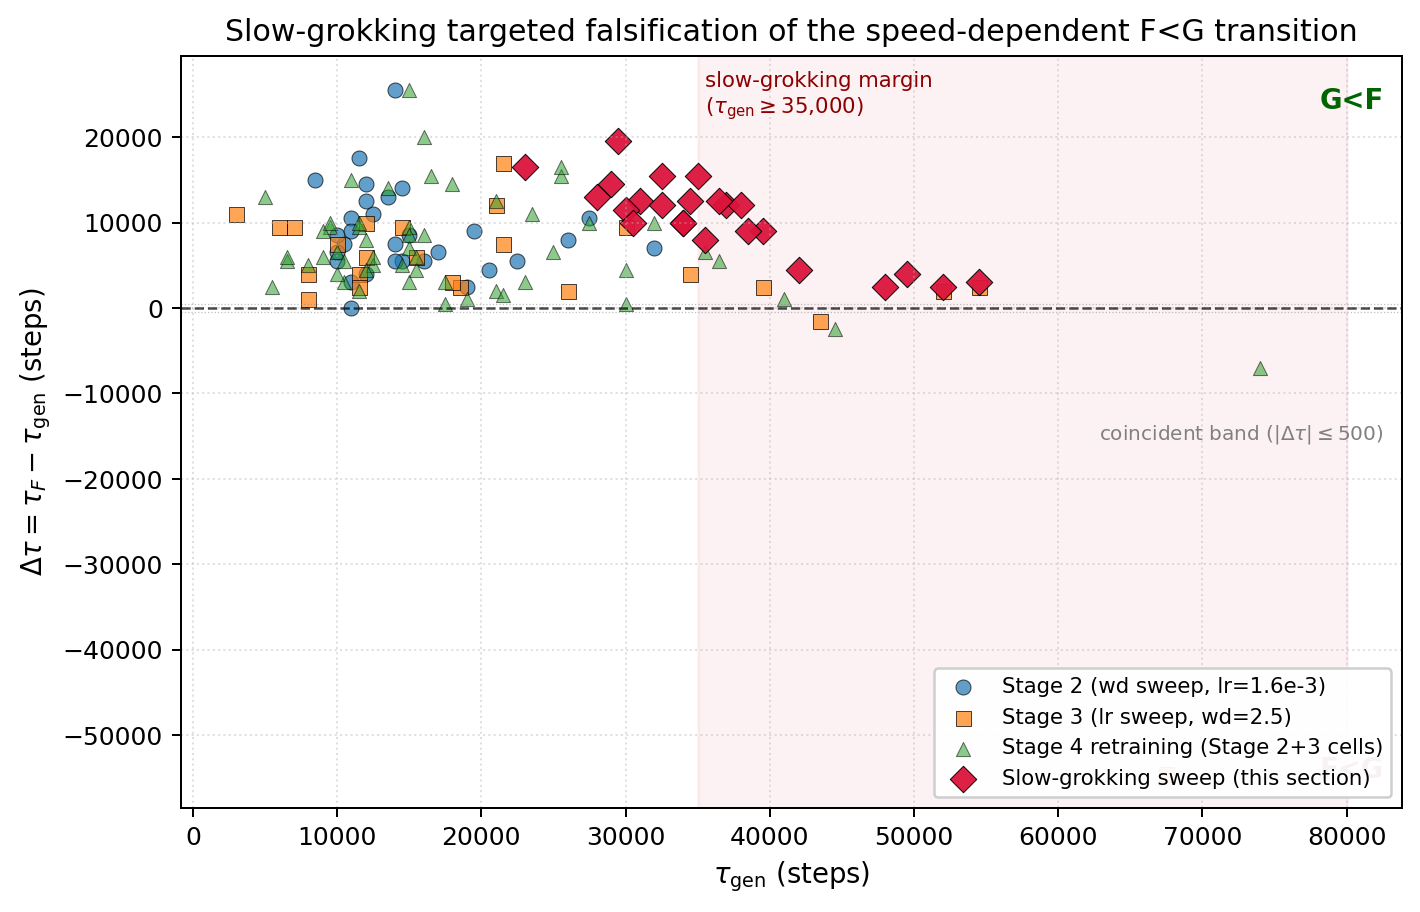
\includegraphics[width=\linewidth]{slow_grokking_scatter.png}
  \caption{%
    \textbf{Targeted slow-grokking sweep falsifies the strong
    form.}
    Scatter of $\Dtau{=}\tauf{-}\taug$ versus $\taug$ for all
    Grokking cells across four sources.
    The crimson diamonds are the targeted slow-grokking sweep
    (24 cells, lr$\in[5.0, 8.0]\!\times\!10^{-4}$, wd$=2.5$,
    seeds $\{42, 7, 2025\}$, max steps $100{,}000$--$120{,}000$);
    blue circles are Stage~2 (wd sweep, lr$=1.6\!\times\!10^{-3}$);
    orange squares are the original Stage~3 (lr sweep, wd$=2.5$);
    green triangles are the Stage~4 retraining of the Stage~2$+$3
    cells.
    The shaded region marks the slow-grokking margin
    ($\taug\geq 35{,}000$).
    All 24 targeted cells fall in the G$<$F half plane
    ($\Dtau>0$); the 12 cells inside the shaded margin are uniformly
    G$<$F.
    The original Stage~3 F$<$G points (orange squares with
    $\Dtau<0$) are not replicated by the cross-hardware re-runs
    visible elsewhere on the plot, consistent with seed/hardware
    variance rather than a systematic regime transition.
  }
  \label{fig:slow_grokking_scatter}
\end{figure}

% ==============================================================
\section{Conclusion}
\label{sec:conclusion}

The Fourier ring in a grokked transformer's embedding PCA is a
lagging indicator of the algorithm it is taken to depict.
By measuring answer-aligned logit Fourier alignment $\taucirc$,
generalization $\taug$, and embedding-Fourier consolidation
$\tauf$ as changepoints within the same runs, we recover the
ordering $\taucirc<\taug<\tauf$ in $48/54$ runs, with roughly
equal spacing between consecutive events
($\approx6{,}000$--$6{,}250$ steps each) and a median
embedding-geometry lag that scales with task difficulty, from
$\approx6{,}000$ steps at $p{=}53$ to $28{,}000$ at $p{=}97$.

The ordering is functional, not cosmetic.
Removing the dominant answer-aligned Fourier subspace between
$\taucirc$ and $\tauf$ costs $0.40$--$0.72$ test accuracy while
matched-energy random removals cost nothing measurable, and a
label-free internal patch reproduces that specificity at the
second-layer components and the final residual stream.
The same removal applied to the token embedding also bites before
$\tauf$: what consolidates late is the visible global geometry,
not the functional Fourier content.

The lag is a stable feature of this setting rather than an
artefact of one slice.
It holds in $212/236$ Grokking runs across two tasks, two primes,
a dense (lr, wd) grid, and every weight-decay and cross-task
slice without exception ($29/30$ with one tie, $30/30$, $21/21$);
a purpose-built slow-grokking sweep closes off generalization
speed as the driver, and a 36-configuration sweep of the
changepoint detector's own hyperparameters leaves the ordering
unchanged wherever $|\Dtau|\geq3{,}000$~steps.

The practical consequence is a caution about a widely used
diagnostic: embedding geometry read as a progress measure
systematically understates how far the computation has advanced.
A clean ring means the algorithm arrived some thousands of steps
ago, not that it is arriving now.

\subsection*{Broader Impact Statement}

This work studies a small-scale neural network training phenomenon.
No immediate harmful applications are foreseen.
Findings may inform training efficiency research by clarifying which
structural changes are or are not necessary for generalization.

% ==============================================================
\bibliographystyle{tmlr}
\bibliography{refs}

% ==============================================================
\appendix
\section{Experimental Details}
\label{app:details}

\subsection{BIC Changepoint Estimator}

We apply an exponential moving average ($\alpha{=}0.15$) to the
$\fcorr$ trajectory, then operate on $\log(1+t)$.
We search all candidate breakpoints in the interior two-thirds of
the sequence, fitting OLS regressions before and after each candidate.
The 4-parameter breakpoint model is accepted if BIC$_{\text{break}}
<$~BIC$_{\text{no-break}}$, where BIC$_k = n\log(\text{RSS}/n)
+ k\log(n)$.
A persistence check requires the post-break slope to exceed 1\% of
the total value range.

\subsection{Null Permutation Estimation}

Each run maintains a fixed NumPy RNG seeded as
$\text{run\_seed}\oplus\texttt{0xDEAD}$, independent of the model
RNG.
We shuffle the $p$ token indices 100 times at every 500-step log
point (the canonical refresh cadence; see
Section~\ref{sec:methods}) to estimate $F_{\mathrm{null,p95}}$.
Sensitivity-analysis configurations using $2{,}500$- and
$5{,}000$-step refresh intervals are reported in
Section~\ref{sec:robustness}.

\subsection{Hyperparameter Values}

\paragraph{Stage~2.}
wd~$\in\{1.20, 1.35, 1.52, 1.71, 1.93, 2.18, 2.45, 2.76, 3.11,
3.50\}$; lr~$=1.6\times10^{-3}$; seeds~$=\{42,7,2025\}$.

\paragraph{Stage~3.}
lr~$\in\{5.00, 6.80, 9.26, 12.6, 17.1, 23.3, 31.7, 43.2, 58.8,
80.0\}\times10^{-4}$; wd~$=2.5$; seeds~$=\{42,7,2025\}$.

% ==============================================================
\section{Complete Timing Results}
\label{app:scatter}

Figure~\ref{fig:tau_scatter} shows the full scatter of $(\taug,\tauf)$
for all 55~Grokking runs.
Points above the diagonal ($\tauf>\taug$) correspond to G$<$F;
the two red star ($\bigstar$) points below are the F$<$G cases discussed in
Section~\ref{sec:results_lr}.
The scatter confirms that the lag $\Dtau=\tauf-\taug$ is
distributed throughout the range 1{,}000--25{,}000 steps with no
obvious bimodal structure.

\begin{figure}[htbp]
  \centering
  
\includegraphics[width=0.58\linewidth]{tau_scatter.png}
  \caption{%
    Scatter plot of $\taug$ vs $\tauf$ for all 55~Grokking runs
    (blue = Stage~2 wd sweep; orange = Stage~3 lr sweep).
    All points above the dashed diagonal are G$<$F.
    The two red star ($\bigstar$) points below the diagonal are the
    F$<$G outliers discussed in Section~\ref{sec:results_lr}.
  }
  \label{fig:tau_scatter}
\end{figure}

% ==============================================================
\section{Per-Cell Detector Sensitivity}
\label{app:sensitivity}

Figure~\ref{fig:percell_heatmap} extends the aggregate
robustness heatmap (Figure~\ref{fig:robustness_heatmap}) to show
P(G$<$F) per cell, allowing inspection of which configurations
drive the RS~$<1$ cases.

\begin{figure}[htbp]
  \centering
  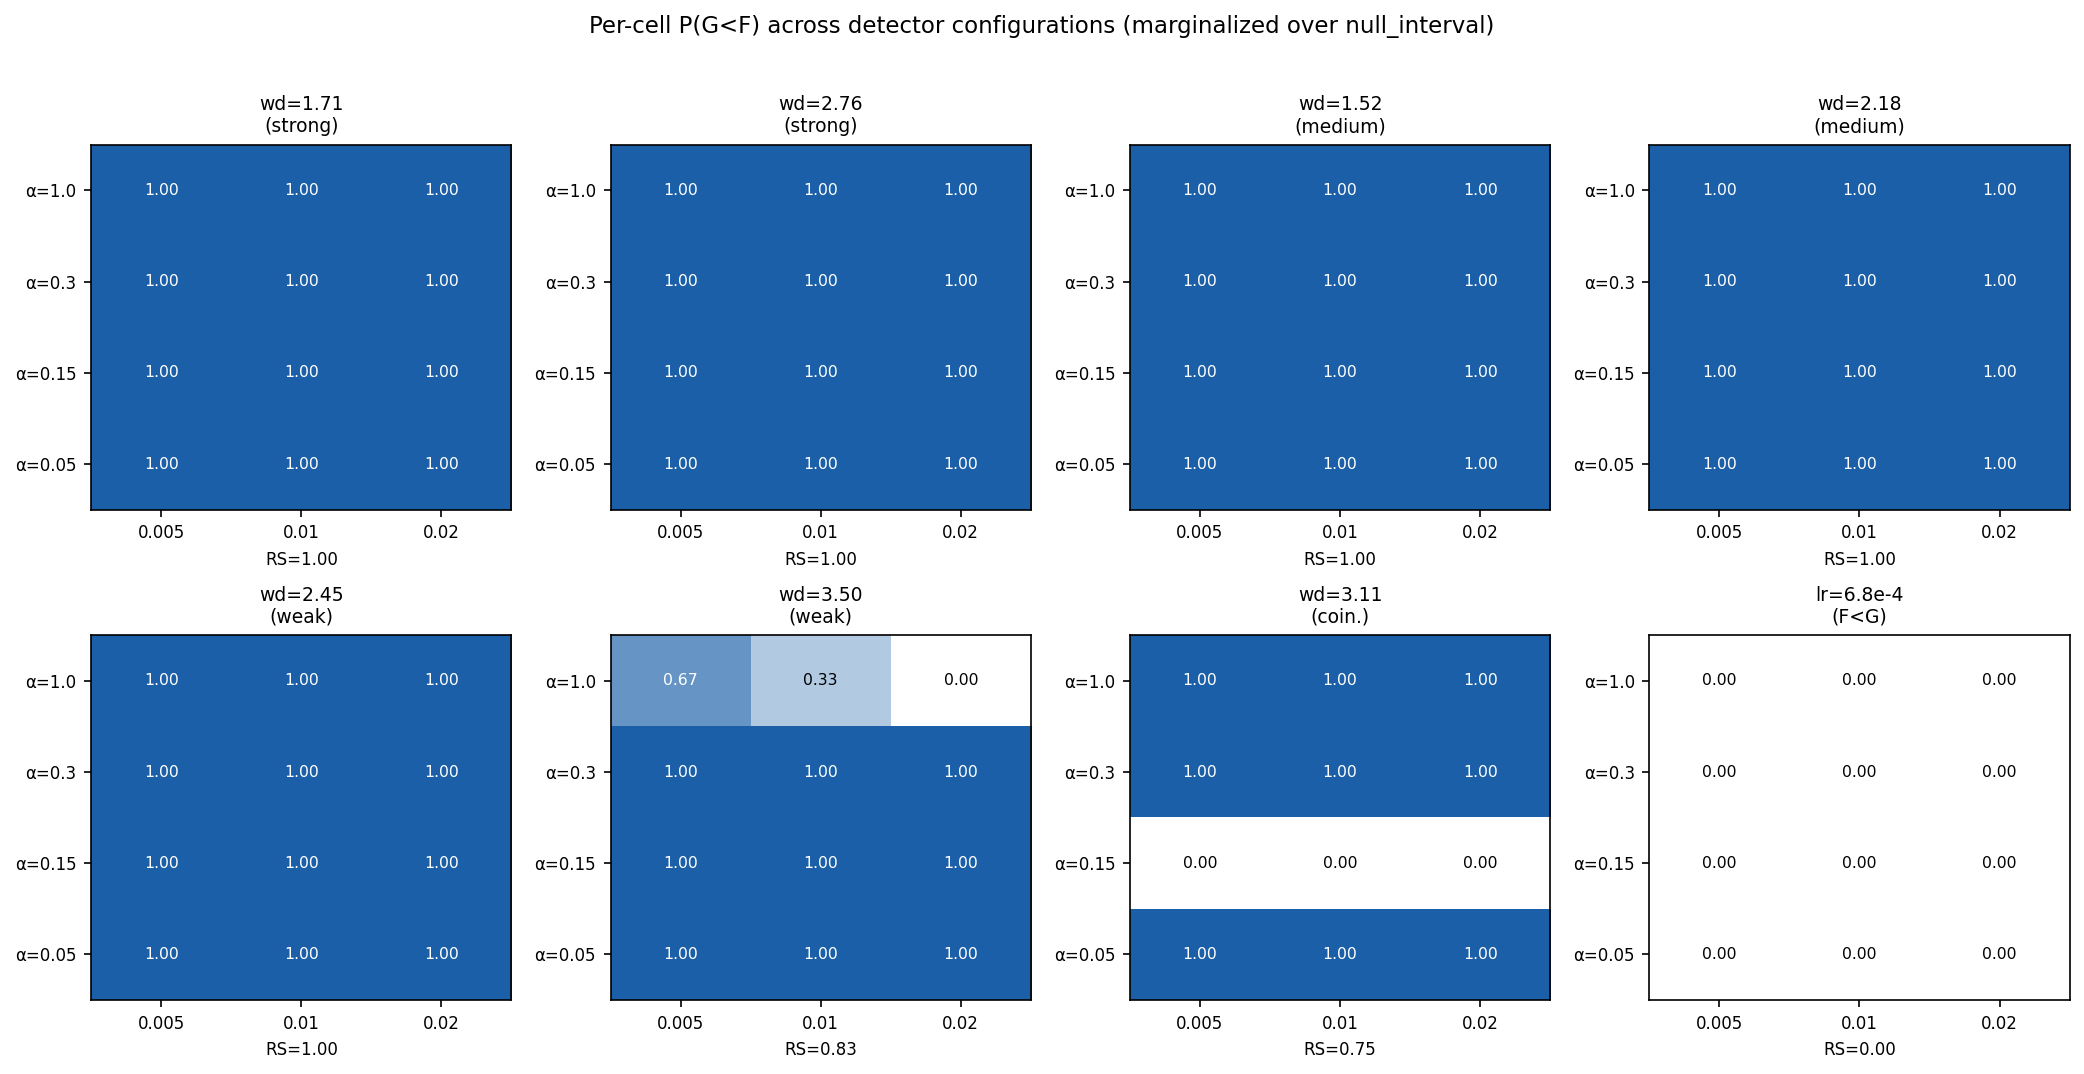
\includegraphics[width=\linewidth]{sensitivity_percell_heatmap.png}
  \caption{%
    Per-cell P(G$<$F) across all 36 detector configurations,
    marginalized over null-update interval.
    Strong and medium G$<$F cells (first four panels) are
    uniformly blue (RS$=1.00$).
    Weak G$<$F cells degrade to \emph{coincident} (not F$<$G)
    under the strictest slope threshold.
    The F$<$G outlier (bottom right) is uniformly red across
    all 36 configurations, confirming that its ordering is stable
    with respect to detector parameters.
  }
  \label{fig:percell_heatmap}
\end{figure}

Figure~\ref{fig:outlier_traj} provides a direct comparison of the
F$<$G outlier trajectory against the strong G$<$F reference cell.

\begin{figure}[htbp]
  \centering
  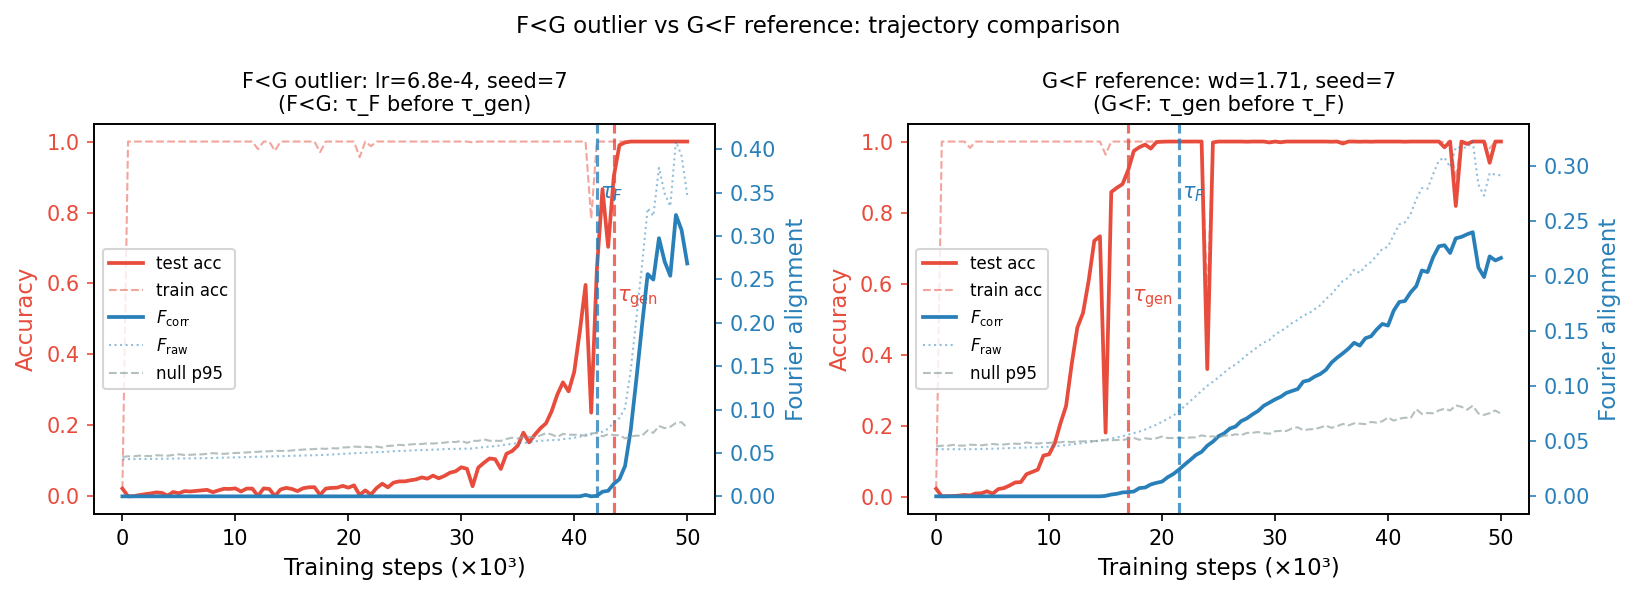
\includegraphics[width=0.90\linewidth]{sensitivity_outlier_trajectory.png}
  \caption{%
    Trajectory comparison: F$<$G outlier (lr$=6.8\!\times\!10^{-4}$,
    seed~7; left) vs.\ a strong G$<$F reference
    (wd$=1.71$, seed~7; right).
    In the outlier, $F_{\mathrm{raw}}$ (dotted blue) hovers near the
    null baseline (grey dashed) throughout training and $\fcorr$ only
    barely exceeds zero near the very late $\taug=43{,}500$.
    In the reference cell, $\fcorr$ shows a clear, sustained rise
    well after the sharp test-accuracy jump.
  }
  \label{fig:outlier_traj}
\end{figure}

% ==============================================================
\section{Reproducibility}
\label{app:reproducibility}

The majority of experiments reported in this paper were run on a
local NVIDIA RTX~4080 Laptop (12~GB VRAM); a smaller subset of
longer-running sweeps was executed on rented cloud GPU instances
(NVIDIA RTX PRO 6000 and NVIDIA A800) accessed remotely via SSH.
All runs used the same PyTorch training loop
(Python~3.11.9, PyTorch~2.5.1+cu121, NumPy~2.4.3,
CUDA~12.1, cuDNN~9.1.0)
with identical model and optimiser code,
and \texttt{torch.backends.cudnn.deterministic=True} is set in the
seeding routine.
\textbf{Bit-exact reproducibility holds within a single GPU/CUDA
configuration but not across them.}
A direct comparison of two independent sweeps on the same nominal
seeds (Stage~4 on a local RTX~4080 vs E3 on a rented A800),
documented in Section~\ref{sec:posthoc} (E3), shows per-cell
$\taug$ shifting by a median of $2{,}000$ steps and the three-way
ordering label reclassifying on $8/60$ cells.
Single-run point estimates of C$<$G and C$<$G$<$F rates therefore
carry an empirically observed $\sim$$9$ percentage points of
cross-hardware run-to-run variance.
Each modular-arithmetic training run terminates in
\mbox{20--45~minutes} at 50{,}000 steps and \mbox{30--75~minutes} at
80{,}000 steps on the local 4080; cloud runs are correspondingly
faster on the larger data-centre GPUs.
The full set of experiments reported here (Stages~2--6 plus the
subtraction pilots) totals approximately 280 runs and
\mbox{$\sim$170~GPU-hours} (aggregated across hardware).

\paragraph{Random seeds.}
Each cell is run with seeds $\{42, 7, 2025\}$.
Seeds are applied uniformly to PyTorch, NumPy, and Python's
\texttt{random} at the start of each run.
The permutation-null estimator uses an independent NumPy generator
seeded with $\texttt{run\_seed}\oplus\texttt{0xDEAD}$ so that null
resampling is reproducible but decoupled from model initialisation.

\paragraph{Hyperparameter table.}
Full hyperparameter values for each stage are listed in
Appendix~\ref{app:details}.
The canonical detector configuration used for all headline numbers
is: null-update interval $=500$~steps, EMA smoothing
$\alpha=0.15$, BIC slope threshold $=0.01$ of the total value range.

\paragraph{Release plan.}
An anonymized supplementary package for review includes the
training scripts, per-run metric trajectories ($\fcorr$, $\flogit$,
test accuracy at every 500-step checkpoint, stored as compressed
\texttt{.npz} files), changepoint scripts, plotting scripts that
reproduce every figure and table in this paper,
\texttt{requirements.txt}, and configuration files for every axis
of variation reported.
A de-anonymized public repository will be released after
acceptance.

% ==============================================================
\section{Future Work}
\label{app:future_work}

We list four natural next steps that extend the empirical scope of
this paper. None is required to support the claims in the main
body, and all are deferred to future work.

\paragraph{F1. Full subtraction sweep.}
Replicate Stages~2 and~3 with operation $(a-b)\bmod p$ for
$p\in\{53,97\}$. Expected cost: $\sim$60 runs, $\sim$45~GPU-hours.
The G$<$F prediction is that the rate should track $\taug$ rather
than the task label.

\paragraph{F2. Architecture-depth scan.}
The depth pilot summarised in the Limitations (Section~\ref{sec:limitations},
``Architecture scope'') shows that the G$<$F ordering reverses at
$n_{\mathrm{layers}}\in\{1,3\}$ on the single canonical operating point
tested.
A full scan should sweep depth and width jointly across multiple
Grokking cells, rather than only the single canonical operating
point used in \texttt{results/arch\_depth/results.csv}.

\paragraph{F3. Online embedding intervention.}
The causal interventions in E7 (Section~\ref{sec:posthoc}) operate
on static checkpoints: we project out Fourier subspaces at inference
time and measure the accuracy drop.
A stronger test would intervene \emph{during training}, clamping
embedding gradients to the null space of the dominant Fourier
harmonics and observing whether generalization is delayed, preserved,
or destroyed.
This would distinguish whether the embedding ring is a passive
by-product of decoder weight decay or plays an active role in
stabilising the learned circuit.

\paragraph{F4. Component-level activation patching.}
The E7 interventions act on output logits (with a basis indexed by
the ground-truth answer class) and on embedding rows (with a basis
indexed by the token value); they establish functional necessity
of the projected subspaces but do not localize where inside the
network the structure is computed.
A label-free, component-level pilot on all 43 probe checkpoints
(reported in Section~\ref{sec:posthoc}, E7, ``Internal activation
patching'') localizes Fourier-specific functional necessity to the
second-layer components and the final residual stream during the
$\taug$--$\tauf$ window.
A systematic version would extend this across the full cell grid
and across depths, resolve per-head (rather than per-module)
contributions, and design on-manifold controls for the embedding
and first-layer sites where a grid-space random control is
inherently destructive.
The probe script is included in the supplementary code
(\texttt{src/analysis/activation\_patching\_probe.py}).

\end{document}
